\chapter{State of the Art}
\label{sec:stateOfTheArt}

To get an idea of possible solutions and the most promising approaches. 
There are many different kinds of vision tasks based on image input.
This chapter introduces to different vision tasks and their approaches to serve as an overview.
Then, the most promising approaches for the rail track prediction use case are selected and further pursued for comparison.

%%%%%%%%%%%%%%%%%%%%% Different appraoches of vision tasks %%%%%%%%%%%%%%%%%%%%%

\section{Different approaches of vision tasks}
\label{sec:differentApproaches}

Many different kinds of vision tasks input image data.
These use cases outline broad guidelines for designing neural network architectures and the workflow of such a model by which the desired output is produced.
\autoref{fig:differentApproaches} shows the outputs of the most commonly used strategies in the literature that might be relevant for rail track prediction or a part of it.
The input image for all models is visualized in \autoref{fig:differentApproaches_classification} without the added text in the top right corner.

\vspace{1cm} % Größerer Abstand zwischen den Reihen

\begin{figure}[H]
    \centering
    
    % Erste Reihe
    \begin{subfigure}{0.328\textwidth}
        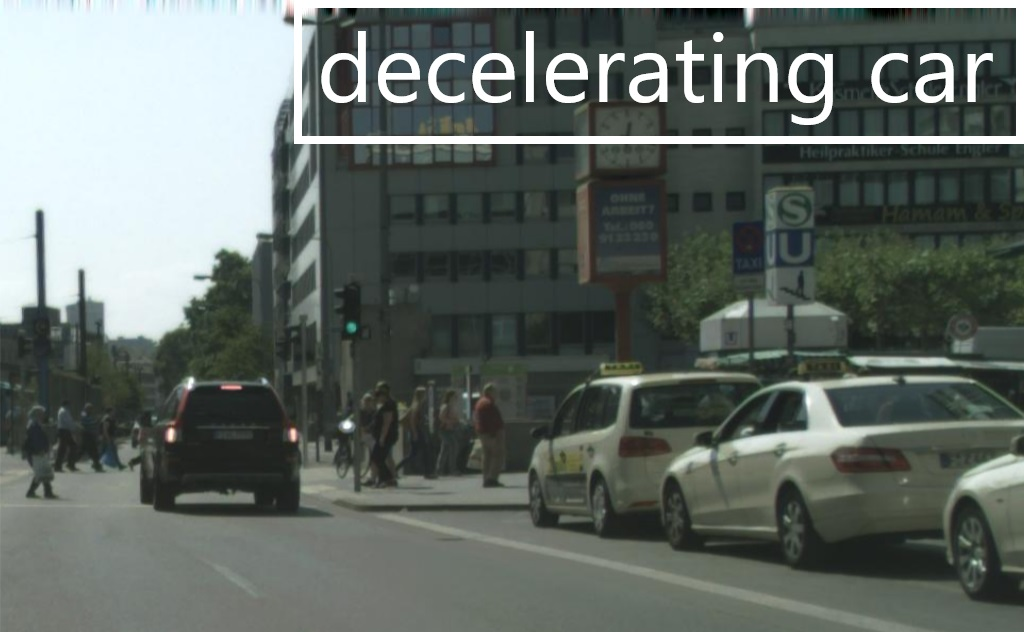
\includegraphics[width=\linewidth]{PICs/differentApproaches/classification_v2.jpg}
        \caption{classification}
        \label{fig:differentApproaches_classification}
    \end{subfigure}
    \hfill
    \begin{subfigure}{0.328\textwidth}
        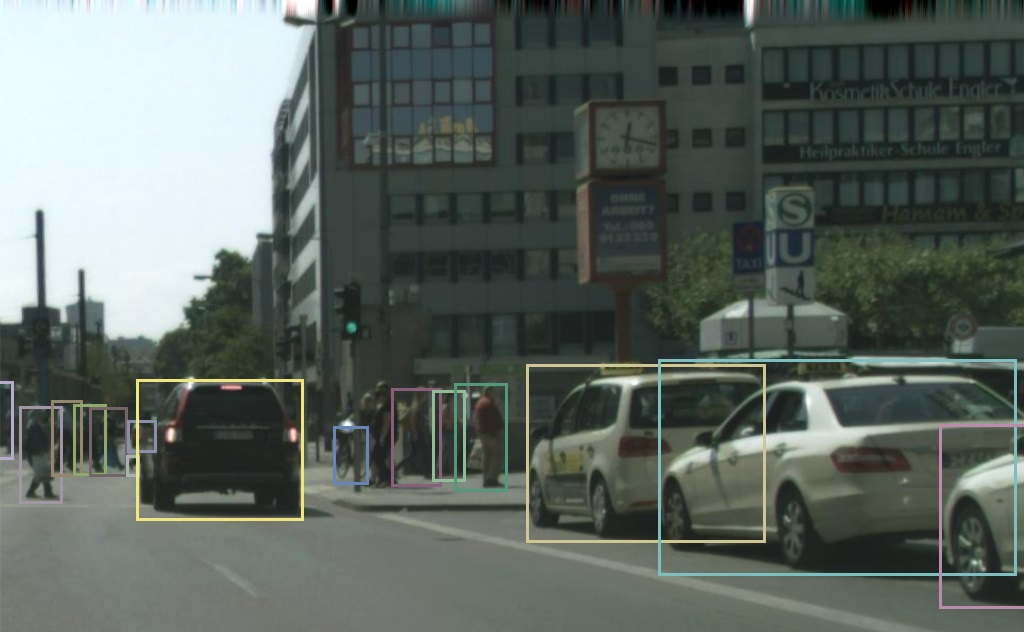
\includegraphics[width=\linewidth]{PICs/differentApproaches/object_detection.jpg}
        \caption{object detection}
        \label{fig:differentApproaches_object_detection}
    \end{subfigure}
    \hfill
    \begin{subfigure}{0.328\textwidth}
        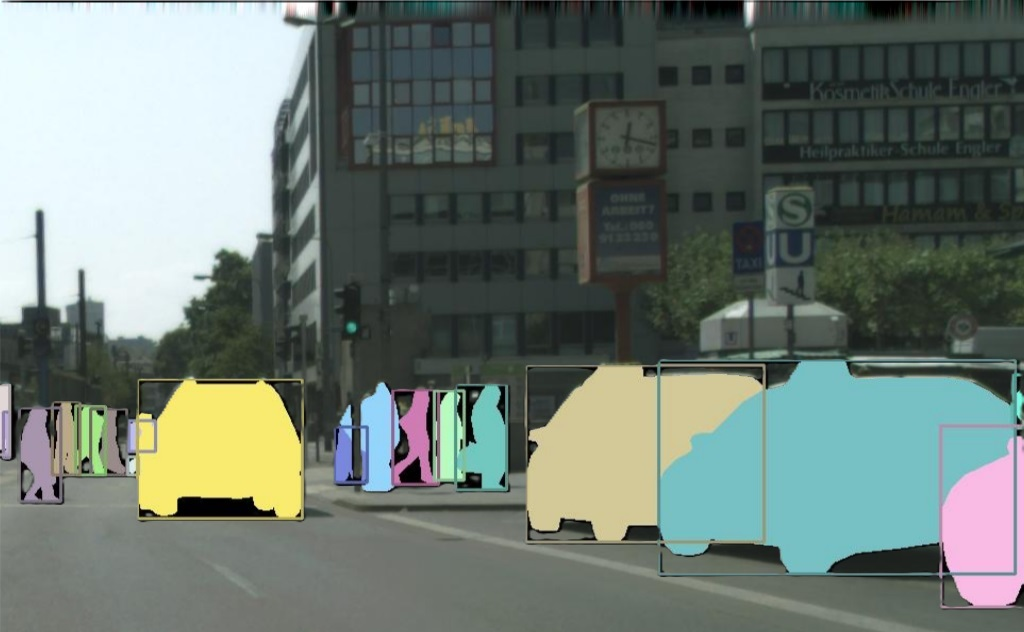
\includegraphics[width=\linewidth]{PICs/differentApproaches/instance_segmentation_v2.jpg}
        \caption{instance segmentation}
        \label{fig:differentApproaches_instance_segmentation}
    \end{subfigure}

    \vspace{0.1cm} % Größerer Abstand zwischen den Reihen

    % Zweite Reihe
    \begin{subfigure}{0.328\textwidth}
        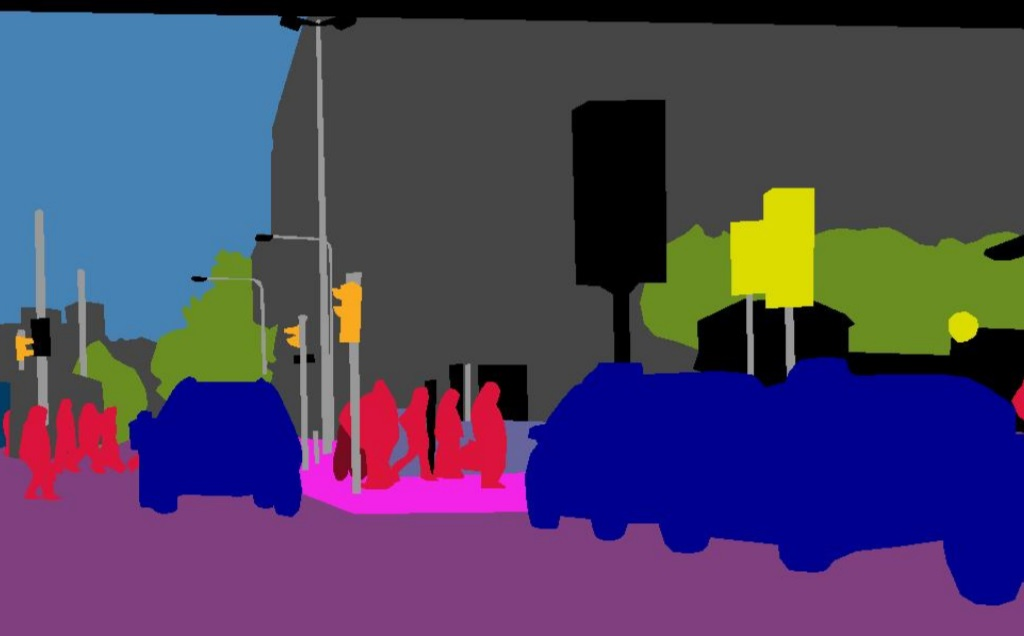
\includegraphics[width=\linewidth]{PICs/differentApproaches/semantic_segmentation.jpg}
        \caption{semantic segmentation}
        \label{fig:differentApproaches_semantic_segmentation}
    \end{subfigure}
    \hfill
    \begin{subfigure}{0.328\textwidth}
        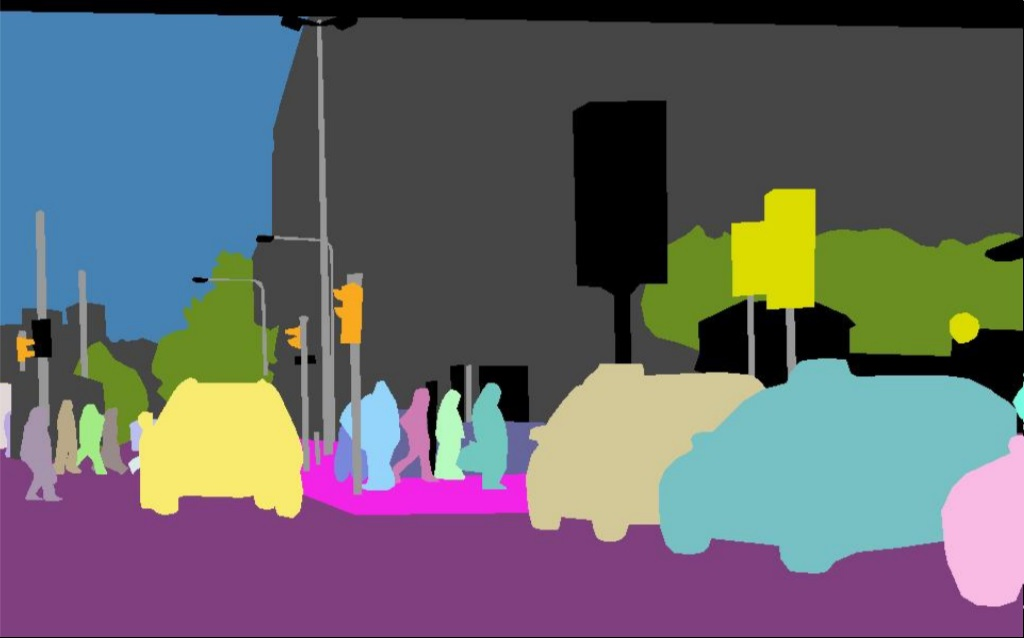
\includegraphics[width=\linewidth]{PICs/differentApproaches/panoptic_segmentation.jpg}
        \caption{panoptic segmentation}
        \label{fig:differentApproaches_panoptic_segmentation}
    \end{subfigure}
    \hfill
    \begin{subfigure}{0.328\textwidth}
        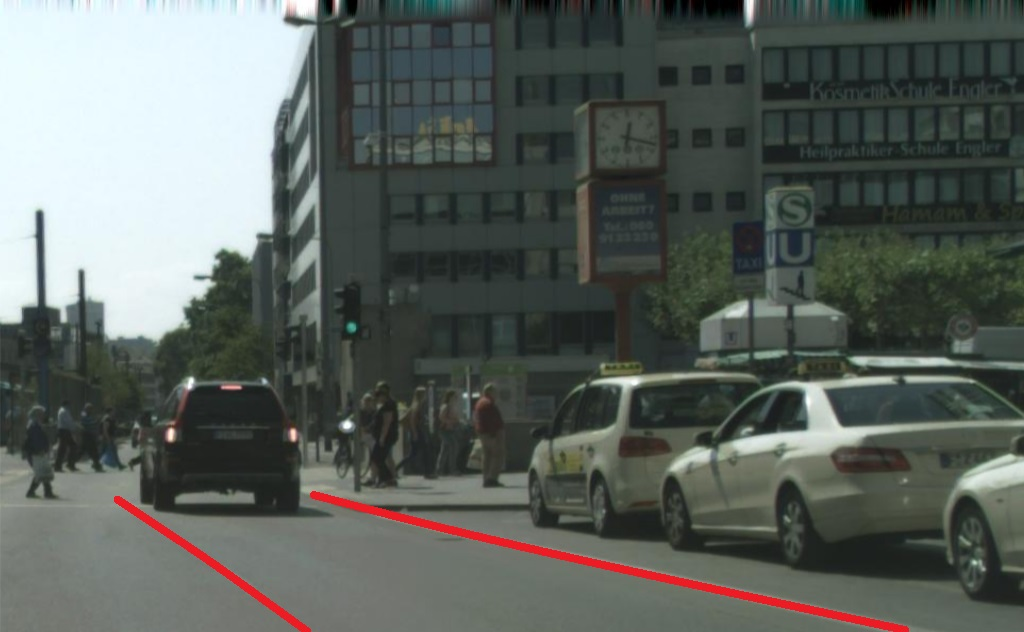
\includegraphics[width=\linewidth]{PICs/differentApproaches/line_detection.jpg}
        \caption{line detection}
        \label{fig:differentApproaches_line_detection}
    \end{subfigure}

    \caption{The most common applications in vision tasks that are supported by neural networks. Shown are \ac{GT} examples for each usage domain. The input image is visualized in (a) without the added text in the top right corner \cite{panopticsegmentation2019}.}
    \label{fig:differentApproaches}
\end{figure}

\clearpage
\noindent\textbf{Classification} describes the scene in the input image with only one label.
\autoref{fig:differentApproaches_classification} shows a possible example with the label added in the top right corner of the input image.
No further information is available from the output of a classification method \cite{cifar100}.

\vspace{1cm} % Größerer Abstand zwischen den Reihen

\noindent\textbf{Object detection} combines classification with localization.
This technique outputs so-called bounding boxes that also include positional information of objects.
Additionally, class labels are assigned to each bounding box which show what has been recognized \cite{panopticsegmentation2019}.

\vspace{1cm} % Größerer Abstand zwischen den Reihen

\noindent\textbf{Instance segmentation} expands on object detection by not just outputting bounding boxes.
It generates binary masks within each bounding box, enabling more accurate identification of the pixels that belong to the object and those that do not.
Regions within the bounding box that are not part of the object are disregarded \cite{panopticsegmentation2019}.

\vspace{1cm} % Größerer Abstand zwischen den Reihen

\noindent\textbf{Semantic segmentation} is a method that outputs a class label for each pixel of the input image.
Consequently, the output consists of a mask with the same width and height as the input image.
An example is shown in \autoref{fig:differentApproaches_semantic_segmentation} with people and cars being two of the output labels.
In this work, semantic segmentation can be used for filtering out the rail track for example \cite{panopticsegmentation2019}.

\vspace{1cm} % Größerer Abstand zwischen den Reihen

\noindent\textbf{Panoptic segmentation} combines semantic segmentation and instance segmentation.
It makes the difference between so-called "things" and "stuff" \cite{panopticsegmentation2019}.
Examples of "things" in \autoref{fig:differentApproaches_panoptic_segmentation} are countable objects like cars and people.
Examples of "stuff" are the road, buildings or the sky.
As with semantic segmentation, this method outputs a pixel-wise classification.
This mask also has the same dimensions as the input image.
However, while semantic segmentation assigns the same class to different instances of the same objects, panoptic segmentation can differentiate between different "things".
\autoref{fig:differentApproaches_panoptic_segmentation} shows that each car or person has its unique class label.

\vspace{1cm} % Größerer Abstand zwischen den Reihen

\noindent\textbf{Line detection} algorithms are usually tailored to filter out lines like road markings or rails.
\autoref{fig:differentApproaches_line_detection} shows a possible output in the road domain of such an algorithm.
Even though in the field of line detection a lot of work has been done in the road domain, the main focus of this work is on applications in the rail domain.
Furthermore, many state-of-the-art papers include outputs in the form of binary masks with the same dimensions as the input image.
While these models solve the line detection problem, they use pixel-wise classification and technically fall into the category of semantic segmentation.
In this work, these papers are therefore reviewed in the corresponding section.
Solely techniques not based on semantic segmentation are included in the line detection section.

\clearpage

\noindent Following a brief description of all the various approaches, it becomes clear that only object detection, semantic segmentation, and line detection are viable options for rail track prediction.
Object detection can be used to filter out switches in the image and their states.
The information if a switch state is left or right can be useful for predicting the leading rail in an application.
Semantic segmentation can be used to identify the track itself on the pixel level.
This solution provides a more intuitive solution for train operators where not only a state is outputted, but the track is visualized in the image.
Ideally, object detection and track segmentation are combined so that only the train's track is displayed.
The third approach, which must not be overlooked is line detection algorithms.
While the output and techniques slightly differ from semantic segmentation, they also provide important pixel-wise information about the track.
As the other approaches are not suitable or relevant for this use case, they are excluded. The next few sections focus on the three techniques mentioned and describe them in more detail.

%%%%%%%%%%%%%%%%%%%%%%%%%%%%%%%%%%%%%%%%%%%%%%%%%%%%%%%%%%%%%%%%%%

%%%%%%%%%%%%%%%%%%%%% Object Detection %%%%%%%%%%%%%%%%%%%%%

\section{Real-time Object detection}
\label{sec:ObjectDetection}

Object Detection models, which result in bounding boxes can be utilized for the detection of rail switches or even switch states.
Therefore these models can be of importance for the implementation of the rail track prediction of this work.
This section provides a brief introduction to various object detection models.
In 2012 \cite{AlexNet2012} showed that deep convolutional networks are capable of extracting abstract feature representations from images in a robust manner.
Enabling accurate classification.
In 2014 \cite{RCNN2014} introduced Regions with CNN features \ac{RCNN}.
Since then the development of CNNs can be grouped into two different detection techniques: "two-stage detectors" and "one-stage detectors" \cite{20yearsSurvey} \cite{surveyObjectDetection} \cite{surveyObjectDetection2019}.

\subsection{Two-stage detectors}

Two-stage detectors usually follow a "coarse-to-fine" process, which firstly includes a region proposal and secondly a classification and a refinement of regions \cite{20yearsSurvey} \cite{surveyObjectDetection} \cite{surveyObjectDetection2019} \cite{twostageObjectDetection}.
Well-known examples are the R-CNN \cite{RCNN2014}, Fast R-CNN \cite{FastRCNN2015}, Faster R-CNN \cite{FasterRCNN2017}, Mask R-CNN \cite{MaskRCNN2017}, and \ac{FPN} \cite{FPN2017_two_stage-detector}.
Even though these models achieve promising accuracy results, they are highly complex, which increases inference time.
Consequently, two-stage detectors are usually unsuitable for real-time-critical applications.
Since all of the use cases of the implementation of this work involve real-time capable applications, the inference time is of great importance.
Therefore two-stage detectors are not further considered for this work.

\subsection{One-stage detectors}

Single-stage detectors or one-stage-detectors combine the classification and localization in one step making them fast enough for real-time applications.
The first single shot detector was the \ac{YOLO} \cite{YOLOv1}, which operates with up to 155 FPS.
\ac{YOLO} is the first approach, which reframed the object detection task as a regression problem.
The introduced model consists of a single neuronal network, allowing end-to-end training.
This model first divides the image into a grid and then simultaneously predicts bounding boxes and the probabilities of classes.
Proving to be a fast object detector, \cite{YOLOv1} presented the beginning of a whole series of real-time capable models.
Since, \cite{YOLOv1} still shows decreased accuracy in the localization of small objects, versions \ac{YOLO}v3 \cite{yolov3}, \ac{YOLO}v4 \cite{yolov4}, \ac{YOLO}9000 \cite{yolo9000}, and \ac{SSD} \cite{SSD_model} particularly focused on this issue.
However, \ac{YOLO}v7 \cite{yolov7} and \ac{YOLO}v9 \cite{YOLOv9} are among the latest real-time object detection models, emphasizing both high speed and improved parameter utilization \cite{20yearsSurvey} \cite{surveyObjectDetection} \cite{surveyObjectDetection2019} \cite{realTimeObjectDetection}.

\subsubsection{YOLO v7}
\label{subsubsec:YOLOv7}

The \ac{YOLO}v7 \cite{yolov7} introduced in 2022 is a subsequent work from the \ac{YOLO}v4 \cite{yolov4}.
It surpasses most object detectors in both accuracy and speed, with inferences from 5 FPS to 160 FPS.
The main contributions of \ac{YOLO}v7 \cite{yolov7} are several methods that increase the accuracy without decelerating inference.
To achieve that it incorporates a planned re-parameterized strategy, which can be utilized for layers in various models.
Furthermore, \ac{YOLO}v7 \cite{yolov7} also uses new label assignment methods called "coarse-to-fine lead head guided label assignment".
Additionally, extend and compound scaling techniques are used.
The introduced methods not only increased speed and accuracy, but also decreased the number of parameters of the model by about 40 \% \cite{yolov7}.
This presents an advantage for this work since the final system is supposed to operate on an embedded device.

\subsubsection{YOLO v9}
\label{subsubsec:YOLOv9}

The \ac{YOLO}v9 \cite{YOLOv9} is yet another follow-up work from \ac{YOLO}v7 \cite{yolov7}.
Released in February 2024, it is the most recent model in the \ac{YOLO} series.
\cite{YOLOv9} states that most models lose information through spatial transformations and layer-by-layer feature extraction.
Therefore, the YOLO v9 model focuses on reversible functions and information bottlenecks.
Consequently, the main contributions of \cite{YOLOv9} are a \ac{PGI} concept, which utilizes auxiliary reversible branches, and a \ac{GELAN}, which further increases the usage of existing parameters.
The proposed models prove to be lightweight while still being accurate and fast, outperforming current real-time object detection models.
The characteristics of these models indicate that they are also applicable to this work.


%%%%%%%%%%%%%%%%%%%%%%%%%%%%%%%%%%%%%%%%%%%%%%%%%%%%%%%%%%%%%%%%%%

%%%%%%%%%%%%%%%%%%%%% Semantic Segmentation %%%%%%%%%%%%%%%%%%%%%

\section{Semantic Segmentation}
\label{sec:SemanticSegmentation}

The first approach to filter out the rail tracks in front of the train was proposed by \cite{firstRailSegmentation2018} in 2018.
A SegNet \cite{SegNet2017} <Quelle: SegNet> inspired network for semantic segmentation is extended with mixed pooling \cite{mixedPooling2014} <Quelle> and \ac{ASPP} from DeepLab \cite{deepLab2018}.
After the proposed semantic segmentation network outputs a binary mask with pixel labels being track or no track, a polygon fitting technique is utilized to refine the tracks further.

In 2019 \cite{railNet2019} <RailNet: A Segmentation Network for Railroad Detection> introduced the RailNet architecture.
This model uses a ResNet-50 \cite{ResNet} backbone and a fully convolutional network <Quelle in TEP-Net> to segment the rail tracks.
The network is designed in a pyramid structure <Quelle: 2017 Feature pyramid networks for object detection>, in which features of every ResNet stage are summed and up-sampled.
This combines low and high-level features, resulting in an enhanced performance.
\cite{railNet2019} <Quelle: RailNet: A Segmentation Network for Railroad Detection> reports higher accuracy than state-of-the-art segmentation models at the time with speeds up to 20 \ac{FPS}.
Tests are made on the introduced \ac{RSDS} dataset further described in <Dataset section>.

In 2019 RailSem19 \cite{railsem19dataset} introduced the first publicly available dataset for the rail domain.
This dataset also includes annotations for semantic segmentation tasks and experimented with a FRRNB model <Quelle: Full-Resolution Residual Networks for Semantic Segmentation in Street Scenes>.
This dataset is widely used in the community when working in the rail domain.

<Quelle: 2020 RailNet: An Information Aggregation Network for Rail Track Segmentation> already uses a subset of RailSem19 in 2020.
Another RailNet model is proposed that uses a VGG16 backbone and an Information Aggregation Module.
<Quelle: 2020 RailNet: An Information Aggregation Network for Rail Track Segmentation> only predicts the rails in RailSem19, other annotations are ignored.
The characteristics of rails like placement and structure are considered.
Therefore the integrated module is implemented to improve spatial relationship between features on both the vertical and horizontal axes.

<Quelle: 2022 Automated Semantic Segmentation for Autonomous Railway Vehicles> also used RailSem19.
The U-Net <Quelle: U-Net> architecture is trained on four different subsets of RailSem19, including 2, 3, 4, or all 19 classes.
Additionally, A cropping method is implemented to account for the difference in resolutions between the recommended one for U-Net and one of RailSem19's images.

<Quelle: 2022 Application of Rail Segmentation in the Monitoring of Autonomous Train’s Frontal Environment> used the RailSet dataset <Quelle: 2022 RailSet: A Unique Dataset for Railway Anomaly Detection>, which is an extension of RailSem19 for segmentation and anomaly detection tasks.
For details of the RailSet dataset please refer to <dataset section>.
<Quelle: 2022 Application of Rail Segmentation in the Monitoring of Autonomous Train’s Frontal Environment> trained U-Net <Quelle: U-Net> and FRNN <Quelle: FRNN> and incorporated horizontal flips and zooming into the data augmentation.

In 2020 <Quelle: Railroad semantic segmentation on high-resolution images> proposed a U-Net-inspired <Quelle: U-Net> semantic segmentation network.
It combines a ResNet-34 backbone and includes connections to the upsampling blocks.
At the deepest level, a \ac{SPP} <Quelle: Spatial pyramid pooling in deep convolutional networks for visual recognition> and on the skip connections squeeze-and-excitation blocks \cite{SqueezeAndExcitation2019} are used.
Tests on RailSem19 \cite{railsem19dataset}, show that it outperforms \cite{railNet2019} <Quelle: 2019 RailNet: A Segmentation Network for Railroad Detection> in accuracy with a speed of 20 \ac{FPS}.
Additionally, <Quelle: Railroad semantic segmentation on high-resolution images> introduced the concept of "possible tracks", which are all paths the train could follow under the assumption that the state of switches cannot be determined.
For this, a rule-based post-processing algorithm is proposed. <Figure xy> shows the concept of possible paths.

\vspace{1cm}

<vielleicht figure possible tracks von Quelle: Railroad semantic segmentation on high-resolution images>

\vspace{1cm}

In 2023 <Quelle: TPE-Net: Track Point Extraction and Association Network for Rail Path Proposal Generation> further investigated the task of possible tracks and introduced Track Point Extraction and Association Network (TPE-Net).
It consists of a DenseNet-inspired architecture, which is trained and tested on RailSem19 and outputs regressed heatmaps besides the segmented rails.
An example of such a heatmap is an image with one channel that shows the probability of each pixel being within a rail track.
The segmentation mask and the heatmaps are then used by a complex post-processing approach.
This process includes track point clustering, the creation of track segments, and the creation of a path tree, which is then used to generate all possible tracks.
Refinement is done by removing redundant paths and polynomial fitting.
Because of the complexity of this system, <Quelle: TPE-Net: Track Point Extraction and Association Network for Rail Path Proposal Generation> reports speeds up to 12 \ac{FPS} making this system unsuitable for real-time applications.
Additionally, it is stated that problems arise when switches are present.

In 2022 \cite{yuan2022railvid} proposed the RailVID dataset, which consists of infrared images instead of \ac{RGB} data to improve the system's abilities in challenging situations such as the absence of ambient light.
The dataset is described in \autoref{subsubsec:railVID} in more detail.
After collecting data, \cite{yuan2022railvid} experimented with widely used \ac{CNN}s for semantic segmentations, like CGNet <Quelle>, DeepLabv3+ <Quelle>, and BiSeNet <Quelle>.
Additionally, an improved BiSeNet architecture is proposed with consideration of the infrared data. Performance is enhanced by added layers to fuse low-level features.

In 2021 <Accurate and Lightweight RailNet for Real-Time Rail Line Detection> proposed another architecture called RailNet.
It consists of an Encoder-Decoder structure incorporating depth-wise convolutions and a Segmentation Soul block, inspired by the context embedding block of BiSeNetV2 <Quelle: BiSeNetV2>.
Additionally, a port processing algorithm is utilized that is based on sliding window detection.
<Accurate and Lightweight RailNet for Real-Time Rail Line Detection> reports speeds up to 74 \ac{FPS} proving that this system is real-time capable.

A topic that could be interesting is anomaly detection because many state-of-the-art approaches use semantic segmentation as a preprocessing step.
<2021 Near Real-time Situation Awareness and Anomaly Detection for Complex Railway Environment> utilizes a BiSeNet architecture for segmenting rails, which is tailored for the anomaly detection task.
This network can detect small objects on the track.
Therefore accuracy is preferred over speed, resulting in a system that is not real-time capable.

\subsection{Example Überschrift}

blindtext

\subsection{Example Überschrift}

blindtext hallo

%%%%%%%%%%%%%%%%%%%%%%%%%%%%%%%%%%%%%%%%%%%%%%%%%%%%%%%%%%%%%%%%%%


\begin{itemize}
    \item Image Classification
    \item Object Detection
    \item Semantic Segmentation (detection und keine direction prediction) hat normalerweise probleme wenn mehrere rails in der scene sind --> weichen schwer trennbar weil der pixelhaufen dazwischen irgendwas ist
    \item Instance Segmentation
    \item panoptic Segmentation
    \item line detection (detection und keine direction prediction) anzahl der rails in einer scene ist das problem
\end{itemize}

Für die nächstem kapitel:\\
was gibt es?\\
was gibt es in der rail domaine?\\


\subsection{Rail Segmentation oder Semantic Segmentation (2 bis 3 Seiten)}

\begin{itemize}
    \item DeepLab V3+
    \item AdapNet++
    \item ...
\end{itemize}

\subsection{Line detection algorithms (2 bis 3 Seiten)}

Rail Detection: An Efficient Row-based Network and A New Benchmark --> hat auch Lane Detection \& Railroad Detection

\subsection{Backbone architectures 2 Seiten}

\begin{itemize}
    \item EfficientNet 1/2 Seite
    \item ResNet 1/2 Seite
    \item MobileNet 1/2 Seite
    \item DenseNet 1/2 Seite
\end{itemize}

\subsection{mögliches Baseline Paper vielleicht (wenn die Aufteilung geändert werden muss)}

\subsection{verwendetes Baseline Paper vielleicht (wenn die Aufteilung geändert werden muss)}

\subsection{Temporal Models (2 Seiten)}

\begin{itemize}
    \item LSTM -> 1 Seite
    \item GRU -> 1 Seite
    \item ...
\end{itemize}

%%%%%%%%%%%%%%%%%%%%% Datasets %%%%%%%%%%%%%%%%%%%%%

\clearpage
\section{Network architectures}
\label{sec:networkArchitectures}

One of the first \ac{CNN} architectures was the \textbf{Le-Net5} \cite{LeNet5}.
This \ac{CNN} was proposed to classify handwritten digits.
It used 5 convolution and pooling layers.
14 years later \ac{CNN}s were rediscovered with the introduction of \textbf{AlexNet} \cite{AlexNet2012} in 2012.
In the \ac{ILSVRC} \cite{ILSVRC15} in 2012 \textbf{AlexNet} outperformed traditional algorithms and showed the potential of \ac{CNN}s.
Consequently, it is often considered the starting point of the \ac{CNN} era in the literature.
Since then research has shown a rapid development of \ac{CNN} architectures, consistently striving for greater accuracy or speed~\cite{networkArchitectureSurvey}.

\vspace{1cm} % Größerer Abstand zwischen den Reihen

\noindent Several major advancements up to now include:

\begin{itemize}
    \item In 2014 two popular architectures were introduced, which still are often used for state-of-the-art comparisons. Firstly, the \textbf{\ac{VGGNet}} \cite{VGGNet2015} used small three-by-three filters and many layers providing a deep network architecture. Secondly, the \textbf{Inception} network or \textbf{GoogLeNet} \cite{InceptionNet}. To extract features in a range of various scales, this architecture utilized different filter sizes.
    \item In 2015 the \textbf{ResNet} architecture \cite{ResNet} introduced the concept of residual learning with shortcut connections. By skipping layers, this framework enabled the training of deeper networks with over a hundred layers \cite{networkArchitectureSurvey}.
    \item In 2016 \textbf{DenseNets} \cite{DenseNets} was introduced to further deal with the problem of vanishing gradients. This architecture implemented a connection between each layer and every following layer ensuring maximum information flow \cite{networkArchitectureSurvey}.
    \item In 2017 \textbf{MobileNets} \cite{MobileNetV1, MobileNetV2, MobileNetV3} was developed for applications in mobile devices. Since hardware with limited capabilities is used, the main focus of MobileNet architectures lies on efficiency. The utilization of depth-wise separable convolutions allowed small model sizes and fast latencies \cite{networkArchitectureSurvey}.
    \item In 2019 \textbf{EfficientNets} \cite{EfficientNet} was introduced to further explore greater trade-offs between accuracy and efficiency, by using scaling methods for model architectures \cite{networkArchitectureSurvey}. 
\end{itemize}

\vspace{1cm} % Größerer Abstand zwischen den Reihen

\noindent Since the \ac{CNN}s are part of a rapidly developing research field, more recent architectures are more interesting for this work.
Because they already solved issues that exist in older models.
Therefore, only the last four mentioned \ac{CNN}s are described in more detail in the next sections.

\subsection{ResNets}

A widely used model architecture in the community is ResNet \cite{ResNet}.
Before this architecture, \ac{CNN}s faced challenges with the vanishing gradient problem, especially in models with a significant depth.
A neural network is generally classified as deep when it includes numerous sequential layers \cite{ResNet}.
To solve that issue ResNet introduced the residual block that is also visualized in \autoref{fig:resnetResidualBlock}.
This block enabled effective training of models with up to 152 layers. Compared to VGGNet ResNet is 8 times deeper but still less complex.
ResNet showed a great performance gain and was therefore granted first place in the classification task of the ILSVRC 2015.
ResNet is supported in Pytorch, which includes variants with 18, 34, 50, 101, and 152 layers \cite{pytorchresnet}. 
However, ResNet models are still resource-intensive because of their size \cite{networkArchitectureSurvey}. 

\begin{figure}[H]
    \centering
    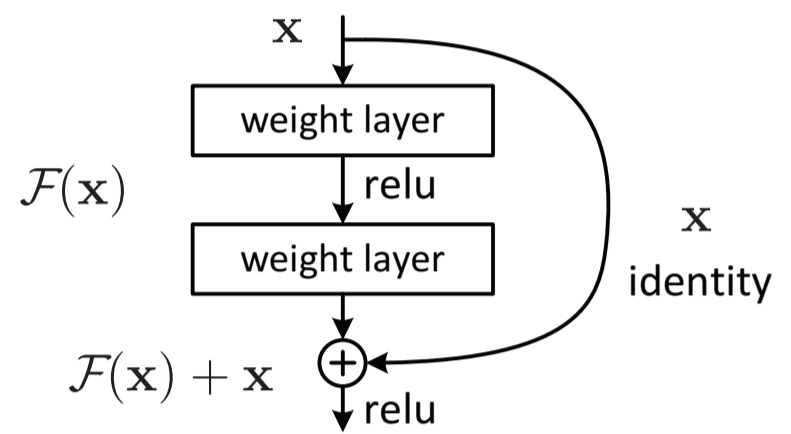
\includegraphics[width=0.5\linewidth]{PICs/backbones/resnet_residualBlock.jpg}
    \caption{ResNet residual block \cite{ResNet}}
    \label{fig:resnetResidualBlock}
\end{figure}

\noindent \autoref{fig:resnetResidualBlock} schematically represents the ResNet's skip connection.
The block has two processes.
One consists of two layers and the other one performs identity mapping.
After that, the outputs are added together.

\subsection{DenseNets}

DenseNet \cite{DenseNets} further explores skip connections and implemented architecture blocks in which each layer is connected to every following layer.
An example of a so-called "dense block" is shown in \autoref{fig:densenetDenseBlock}.
Compared to ResNet, this model connects outputs via concatenation instead of addition.
Between dense blocks, there are the so-called "transition layers", consisting of one convolutional and then one pooling layer.
This architecture allows deeper \ac{CNN}s which result in more accuracy and efficiency.
DenseNet showed great results with the introduced technique because their blocks further tackle the vanishing gradient problem with feature reuse.
PyTorch includes DenseNet model variants with 121, 161, 169, 201 \cite{pytorchdensenet}.

\begin{figure}[H]
    \centering
    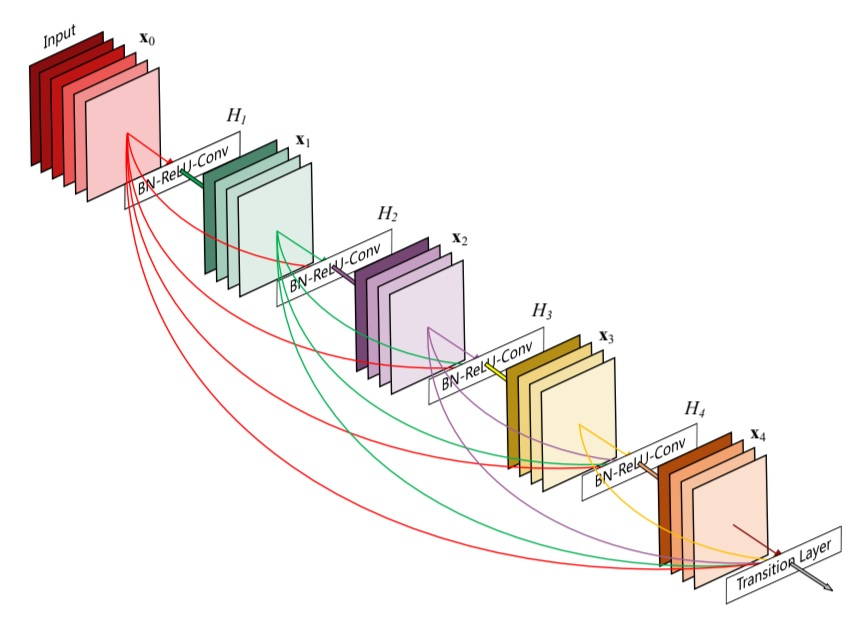
\includegraphics[width=0.5\linewidth]{PICs/backbones/densenet_denseBlock.jpg}
    \caption{DenseNet dense block \cite{DenseNets}}
    \label{fig:densenetDenseBlock}
\end{figure}

\subsection{MobileNetV3}

The goal of the MobileNet series \cite{MobileNetV3} is to efficiently operate on limited hardware for example on mobile devices.
Therefore the main focus of these models is to be as lightweight as possible \cite{networkArchitectureSurvey}, meaning the reduction of parameters and ensuring real-time capabilities while maintaining comparable accuracy.
There are 3 versions of MobileNets and each one builds upon and extends its predecessor.
To achieve a reduced size version 1 utilizes depth-wise separable convolutions.
These blocks of convolutions consist of two steps. First, a depth-wise convolution, where a kernel is deployed on each channel, followed by a point-wise convolution, where a 1x1 kernel combines the output from the first step \cite{networkArchitectureSurvey}.
MobileNet V2 then added a layer with a 1x1 kernel before the depth-wise convolution and a residual connection to create its so-called bottleneck blocks.
A bottleneck block from MobileNetV2 is shown in \autoref{fig:mobileNetV2Block}.

% Bild von MobileNet
\begin{figure}[H]
    \centering
    \begin{subfigure}{0.6\textwidth}
        \centering
        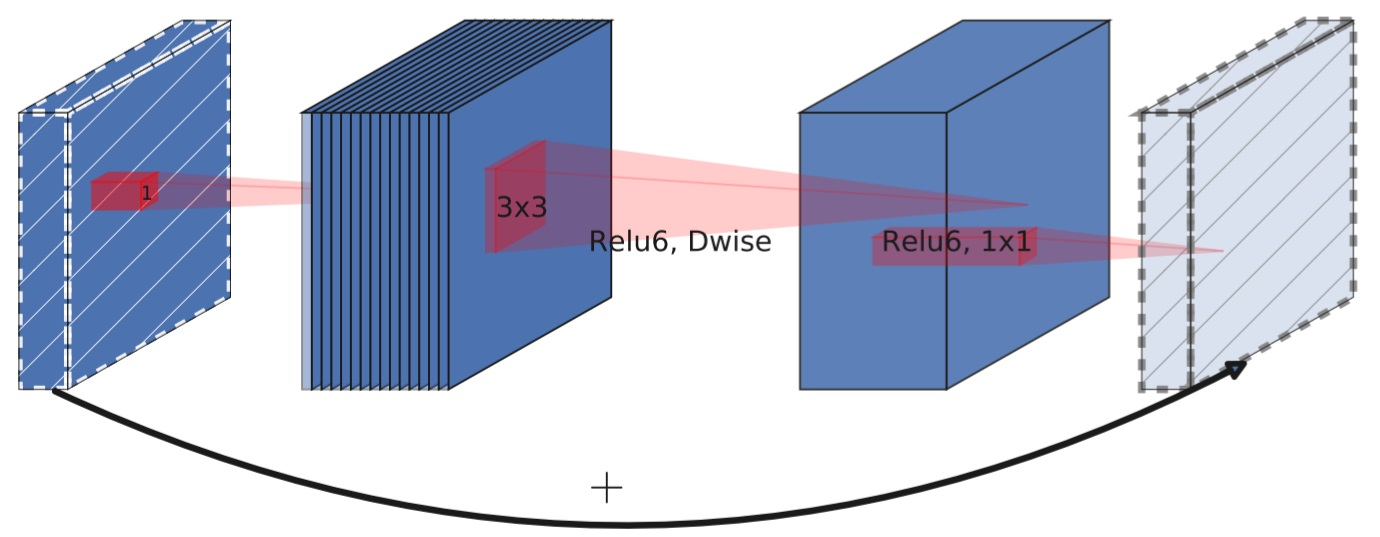
\includegraphics[width=\linewidth, keepaspectratio]{PICs/backbones/mobilenetv2_bottleneck.jpg}
        \caption{}
        \label{fig:mobileNetV2Block}
    \end{subfigure}
    \qquad
    %\hspace*{0.02\textwidth} % Abstand manuell steuern
    \begin{subfigure}{0.6\textwidth}
        \centering
        \vspace{0.8cm}
        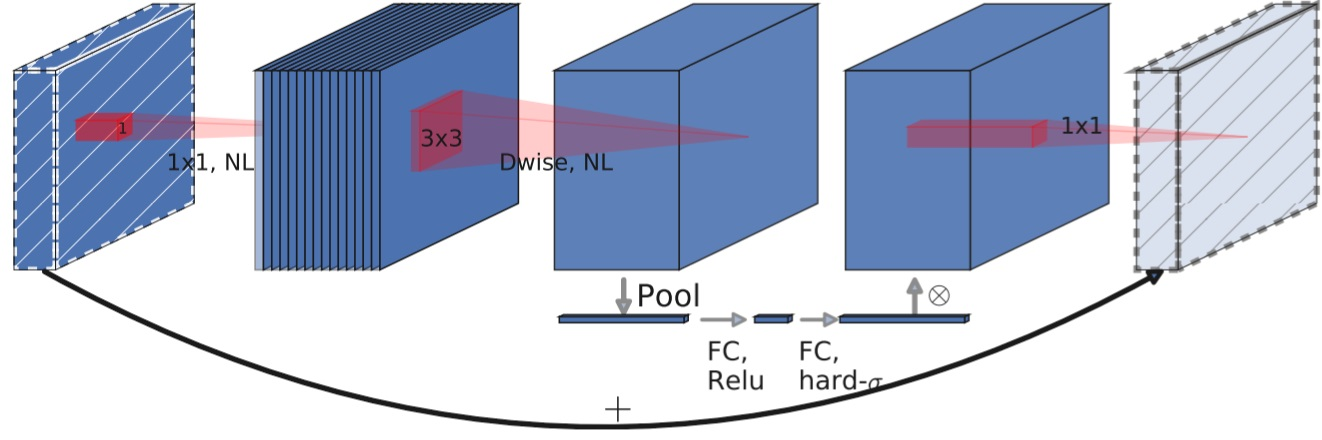
\includegraphics[width=\linewidth, keepaspectratio]{PICs/backbones/mobilenetv3_bottleneck_SE.jpg}
        \caption{}
        \label{fig:mobileNetV3Block}
    \end{subfigure}
    \caption{MobileNet V2 and V3 Blocks \cite{MobileNetV3}: \textbf{(a)} MobileNetV2 bottleneck block, \textbf{(b)} MobileNetV3 bottleneck block with added Squeeze-and-Excite block}
    \label{fig:mobileNetBlocks}
\end{figure}


\noindent MobileNet V3 added optional blocks called Squeeze-and-Excite, which is illustrated in \autoref{fig:mobileNetV3Block}. 
These blocks can be added to any \ac{CNN} and consist of a global pooling layer and two fully connected layers with a ReLu and a Sigmoid activation function respectively.
After that, the output of this additional block is multiplied by the input feature map of the SE block.
This enables the weighing of specific channels \cite{SqueezeAndExcitation2019}.
Additionally, for the MobileNet V3 a Network Search is used to find optimal network structures and experiments with various activation functions have been conducted \cite{MobileNetV3}.

MobileNets allow flexible usage with the so-called width or in V3 depth multiplier, which is a hyperparameter for controlling the number of feature maps in layers.
MobileNet V1 and V2 additionally offer the resolution multiplier, which controls the resolution of layers.
Both the MobileNetV3\_small and MobileNetV3\_large are supported in PyTorch \cite{pytorchmobilenetv3}.

\subsection{EfficientNets}

EfficientNet \cite{EfficientNet} further investigates methods to find \ac{CNN} architectures optimized for efficiency.
Inspired by MobileNet V3 the models also deploy residual bottleneck convolutions.
\cite{EfficientNet} calls such a block an "MBConv".
Since \cite{EfficientNet} observed the correlation between performance improvement and model scaling, the idea is to strategically adjust the depth, width, and resolution of a network.
\autoref{fig:efficientNet_scaled} visualizes these parameters in an example network.
Consequently, a scaling method is introduced, which uses a so-called "compound coefficient".
The resolution as well as the depth and width are uniformly scaled with this technique, resulting in eight variants of EfficientNet.
The different versions, starting with B0 and ending with B7, have increasing parameters.
Since this work focuses on lightweight architectures the most interesting models are the first four (B0, B1, B2, B3).
All variants of the EfficientNet are included in the PyTorch library \cite{pytorchefficientNets}.


% Bild von EfficientNet
\begin{figure}[H]
    \centering
    \begin{subfigure}{0.4\textwidth}
        \centering
        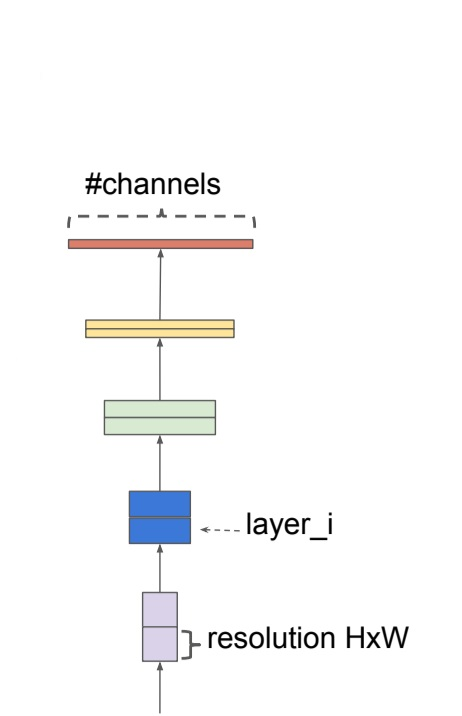
\includegraphics[width=\linewidth, height=7cm, keepaspectratio]{PICs/backbones/EfficientNet_baseline.jpg}
        \caption{network before scaling method}
        \label{fig:efficientNet_baseline}
    \end{subfigure}
    \qquad
    %\hspace*{0.02\textwidth} % Abstand manuell steuern
    \begin{subfigure}{0.4\textwidth}
        \centering
        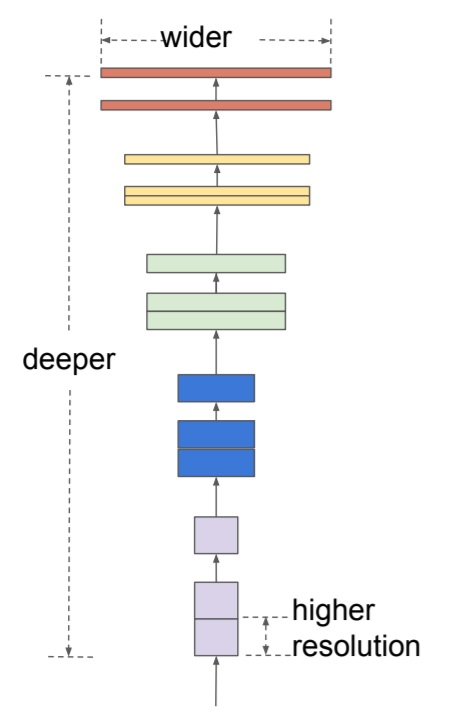
\includegraphics[width=\linewidth, height=7cm, keepaspectratio]{PICs/backbones/EfficientNet_scaling.jpg}
        \caption{scaling parameters of a network according to \cite{EfficientNet}}
        \label{fig:efficientNet_scaled}
    \end{subfigure}
    \caption{Systematic visualization of scaling parameters of a network \cite{EfficientNet}}
    \label{fig:efficientNet_networks}
\end{figure}

%%%%%%%%%%%%%%%%%%%%%%%%%%%%%%%%%%%%%%%%%%%%%%%%%%%%%%%%%%%%%%%%%%

%%%%%%%%%%%%%%%%%%%%% Datasets %%%%%%%%%%%%%%%%%%%%%

\clearpage                                                       % Beginne neue Seite
\section{Datasets}
\label{sec:datasets}

Datasets are essential for the development of autonomous driving systems, particularly for training and testing algorithms or neural networks.
Typically, raw sensor data is collected from real-world driving scenarios, providing a realistic environment that reflects potential situations the system may encounter in future applications.
This allows for more accurate modeling and evaluation of the system's performance under real conditions.
A common approach to solving problems in autonomous driving systems is using vision-based machine learning algorithms ~\cite[S.~1221]{railsem19dataset}.
These applications typically rely on camera-based data to address various challenges ~\cite[S.~1221]{railsem19dataset}.

Since, autonomous vehicles are increasingly considered a groundbreaking technology of the future \cite{FraunhoferInstituteforCognitiveSystemsIKS} a lot of work is put in the development of such systems.
However often the main focus of this quickly evolving field is on road vehicles, like cars or trucks.
Therefore, most publicly available datasets focus on this application and primarily reflect scenarios in road traffic \cite[S.~1221]{railsem19dataset}.

\subsubsection{Classification Datasets}

There are a couple of public datasets for different \ac{CV} applications. The data of the following datasets are especially gathered for classification tasks.

% ---------------------------------------- Table: Datasets for Classification ----------------------------------------
\begin{table}[H]
\centering
\caption{Datasets for Classification}\label{tab_datsets_classification}
\begin{tabular}{| p{0.3\linewidth} | p{0.3\linewidth} | p{0.3\linewidth} |}\hline
Dataset & Labels & Number of relevant images\\\hline
CIFAR 100 & trains & 600\\\hline
PASCAL VOC2012 & trains & 544\\\hline
Microsoft COCO & trains & 3745\\\hline
1000 ImageNet & \begin{tabular}[c]{@{}l@{}}electric\_locomotive, \\ steam\_locomotive, \\ bullet\_train\end{tabular} & 6722\\\hline
Open Images Dataset V4 & train & 9284\\\hline
\end{tabular}
\end{table}
% --------------------------------------------------------------------------------------------------------------------


\textit{CIFAR 100} dataset \cite{cifar100} consists of small images with pixel size 32x32. This dataset includes 600 images with the label \textit{trains}.
In \textit{PASCAL VOC2012} \cite{pascal2015} there are 544 images labeled \textit{trains}.
\textit{Microsoft COCO} \cite{Lin2014MicrosoftCC} has 3745 images with the class \textit{trains}.
Additionally, there are classes like \textit{traffic lights} and \textit{stop sign}, however theses are not useful to the task of this work because they are from the street domain and not the rail domain.
\textit{1000 ImageNet} \cite{ImageNet2015} includes labels like \textit{electric\_locomotive} (4330 images), \textit{steam\_locomotive} (1187 images) and \textit{bullet\_train} (1205 images).
\textit{Open Images Dataset V4} \cite{openImagesV42018} consists of more than 9.2 million images, annotated with bounding boxes.
Included are 10506 \textit{train}-labels in 9284 images.
However, there are no other significant labels relevant to the rail domain.
Additionally, the dataset contains labels for toy trains, which could pose potential challenges.

\subsubsection{Semantic Segmentation}

Semantic segmentation labels are often refereed to as dense or pixel-wise annotated data.
These datasets are characterized by the fact that each pixel in their images is assigned to a class.

% ---------------------------------------- Table: Datasets for Semantic Segmentation ----------------------------------------
\begin{table}[H]
\centering
\caption{Datasets for Semantic Segmentation}\label{tab_datasets_semanticSegmentation}
\begin{tabular}{| p{0.3\linewidth} | p{0.3\linewidth} | p{0.3\linewidth} |}\hline
Dataset & Labels & Number of relevant images\\\hline
Cityscapes & rail track, train & 284\\\hline
Mapillary Vistas & \begin{tabular}[c]{@{}l@{}}construction-flat-rail-track, \\ object-vehicle-on-rails\end{tabular} & 710\\\hline
COCO-Stuff & platform, railroads, train & 8615\\\hline
KITTI & rail tracks, train & 65\\\hline
\end{tabular}
\end{table}
% ---------------------------------------------------------------------------------------------------------------------------

The \textit{Cityscapes} dataset \cite{cityscapes2016} is commonly used for benchmarks when it comes to road scenes.
It has 35 different labels of which two are \textit{rail track} (131 labels in 117 images) and \textit{train} (194 labels in 167 images).
The \textit{rail track} does not differ between the rails and track bed.
\textit{Mapillary Vistas} \cite{mapillaryVistas2017} also has more labels, but again only two are rail related ones.
\textit{construction-flat-rail-track} is annotated in 710 images and \textit{object-vehicle-on-rails} occurs 272 times.
\textit{COCO-Stuff dataset} \cite{COCO-StuffDataset} includes the same 182 classes like the \textit{Microsoft COCO} \cite{Lin2014MicrosoftCC} but as dense labels.
The rail relevant ones are \textit{railroad} (2839) and \textit{train} (4761).
There is a third rail related label \textit{platform}, however this is a very general label because this can by any plane.
\textit{KITTI} \cite{kittiDataset2018} has the same dense labels like \textit{Cityscapes} \cite{cityscapes2016}.
Likewise, the rail relevant ones are 47 \textit{rail track} and 18 \textit{train} labels.

% Problems with general datsets
These are commonly used datasets in \ac{CV} tasks. However there are there are three main issues when it comes to solving the track prediction use case presented in this work.
Firstly, there is not enough data because the amount of included rail relevant labels is relatively low in each dataset.
Secondly, the labels present are not suitable for training a track prediction algorithm. In this case only the rails, rail tracks or track beds are needed.
Thirdly, the images of the presented datasets are taken out of passengers and pedestrian views. Additionally there are some road views \cite{Hadded.2022}.

% Birds eye views und sign datasets
The datasets mentioned before are very general with a vast amount of different labels.
However there are some datasets specially captured for the rail domain.
As with the other datasets, it is important to consider what specific tasks the datasets are intended to be used for.
There are some datasets captured in the birds eye view to detect damages like cracks in rails \cite{rail5k2021} \cite{ma2024cross} or even some to detect garbage in grooved rails \cite{Huang_2021}. Then there are datasets in ego-perspective of the train driver like \textit{FRSign} \cite{Harb2020FRSignAL} or \textit{GERALD} \cite{leibner2023gerald}, which are created for detecting different traffic lights on French and German railways.

% Überleitung mit Perspective Problem zu ego-perspective datasets
This work deals with Rail Track Prediction, so the system should predict the direction of the track in front of the train. For this particular use case it is most advantages when the dataset is recorded out of the driver cabin in ego-perspective, because it offers a clear sight of the rails in front of the train. Therefore the data has to reflect scenarios, which are comparable. Since the view of the captured images represents a key factor, the before mentioned dataset become unsuitable. An additional reason why these datasets cannot be used for this work is the fact that they are created for different use cases.
Other datasets which deal with the perception in a rail domain environment and are captured in the right perspective are discussed in the following paragraphs.

% ================= Richtige datasets =================

% RailSem19
\subsubsection{RailSem19}
\textit{RailSem19} \cite{railsem19dataset} is the first publicly available dataset fitted for environments in the rail domain. It consists of 8500 annotated images which are gathered from YouTube videos. All of these images are captured in the ego perspective of the train driver, which makes it suitable for the use case of this work. Additionally there are both bounding box labels and dense labels included for object detection and semantic segmentation. The bounding box labels are: \textit{guard-rail; rail; traffic-signal-front; traffic-signal-back; traffic-sign-front; crossing; train; platform; buffer-stop; switch-indicator; switch-static; switch-left; switch-right; switch-unknown}. Important for predicting the direction of the train are the switch labels, because  it gives valuable information. The \textit{switch-unknown} label is used when there is a switch visible but it is unclear in which direction the train would proceed. The presents of this label is mainly due to the high noise levels of the images of YouTube videos.
The dense labels of RailSem19 are: \textit{road; sidewalk; construction; tram-track; fence; pole; traffic-light; traffic-sign; vegetation; terrain; sky; human; rail-track; car; truck; track-bed; on-rails; rail-raised; rail-embedded; void}. In the case of dense labels the labels \textit{tram-track; rail-track; track-bed; on-rails; rail-raised; rail-embedded} are of importance for predicting the direction of trains and trams.
Another advantage is that very diverse environments have been used for this dataset. The creators of \textit{RailSem19} took images from 38 different countries in all four seasons and weather conditions. Additionally, the focus was not only on rails but also on trams, providing a very diverse reflection of rail scenarios and not limiting the use on a specific use case.

\begin{figure}[H]
    \centering
    
    % Erste Reihe
    \begin{subfigure}{0.328\textwidth}
        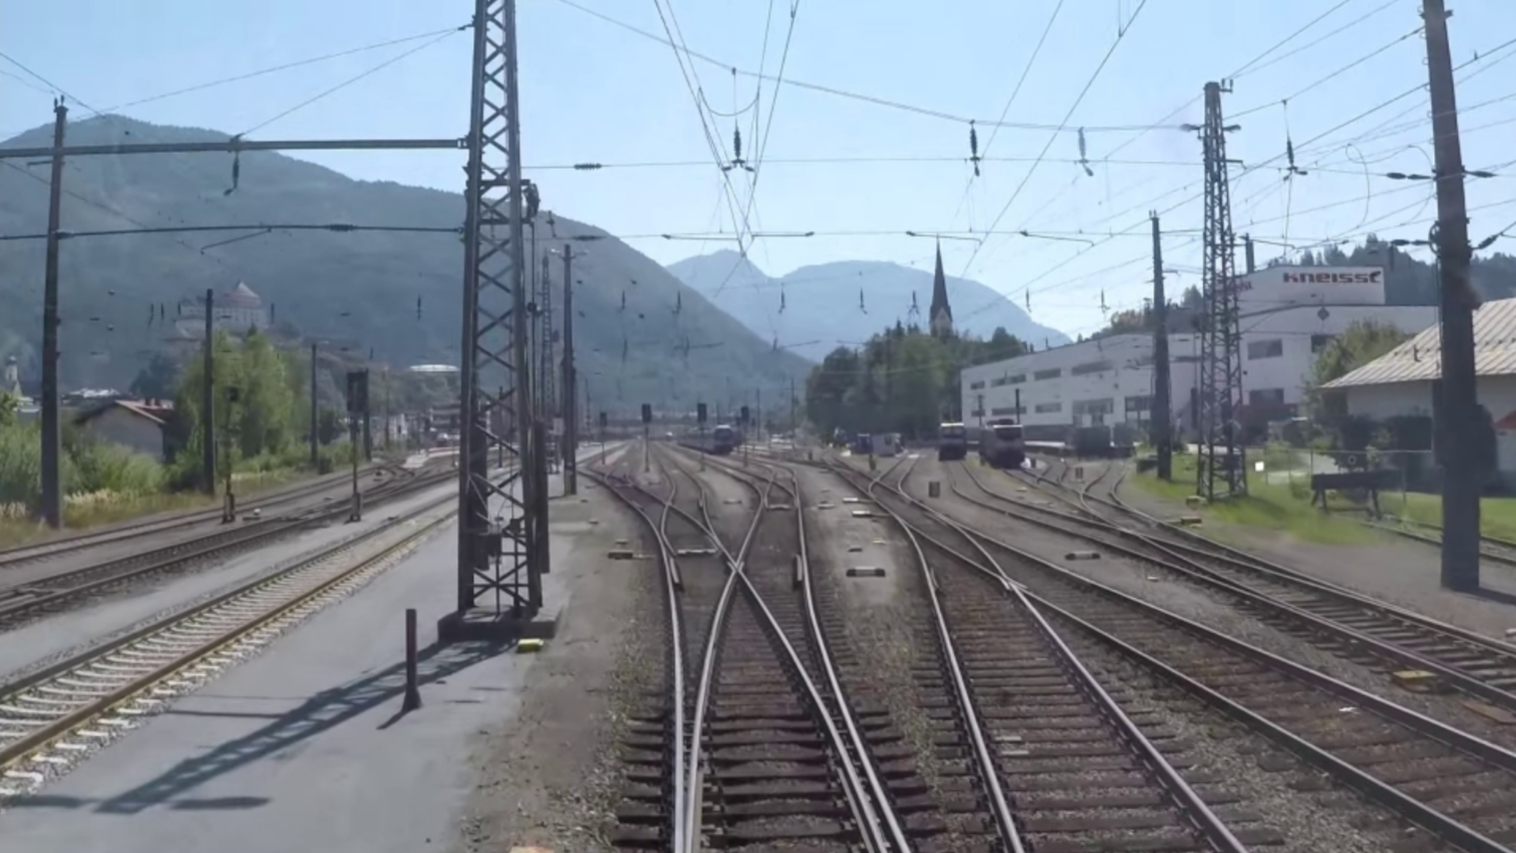
\includegraphics[width=\linewidth]{PICs/datasets/RailSem19_dataset/RailSem19_Bild1.png}
    \end{subfigure}
    \hfill
    \begin{subfigure}{0.328\textwidth}
        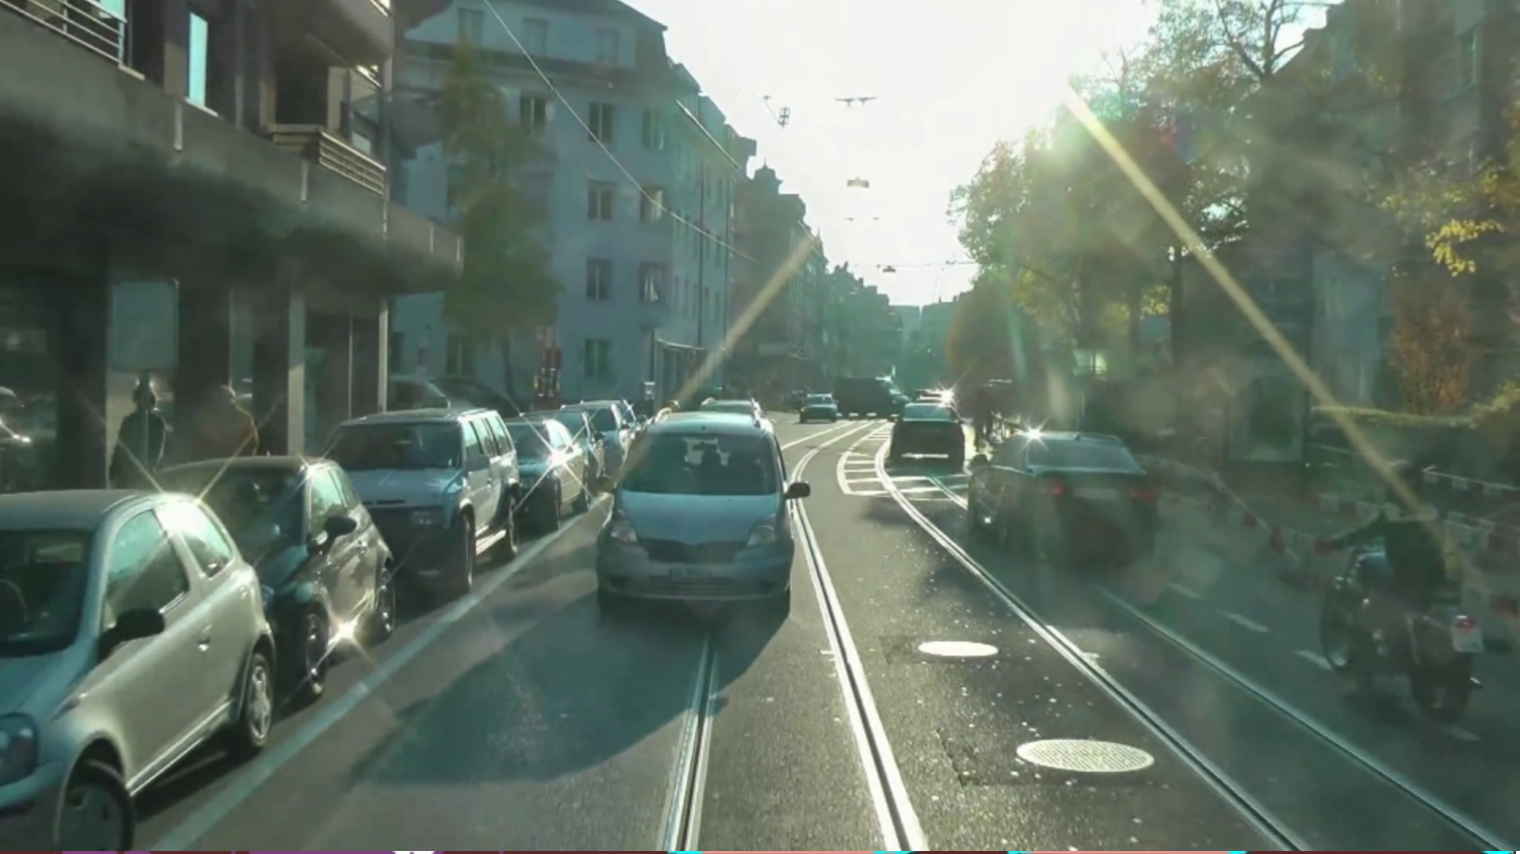
\includegraphics[width=\linewidth]{PICs/datasets/RailSem19_dataset/RailSem19_Bild2.png}
    \end{subfigure}
    \hfill
    \begin{subfigure}{0.328\textwidth}
        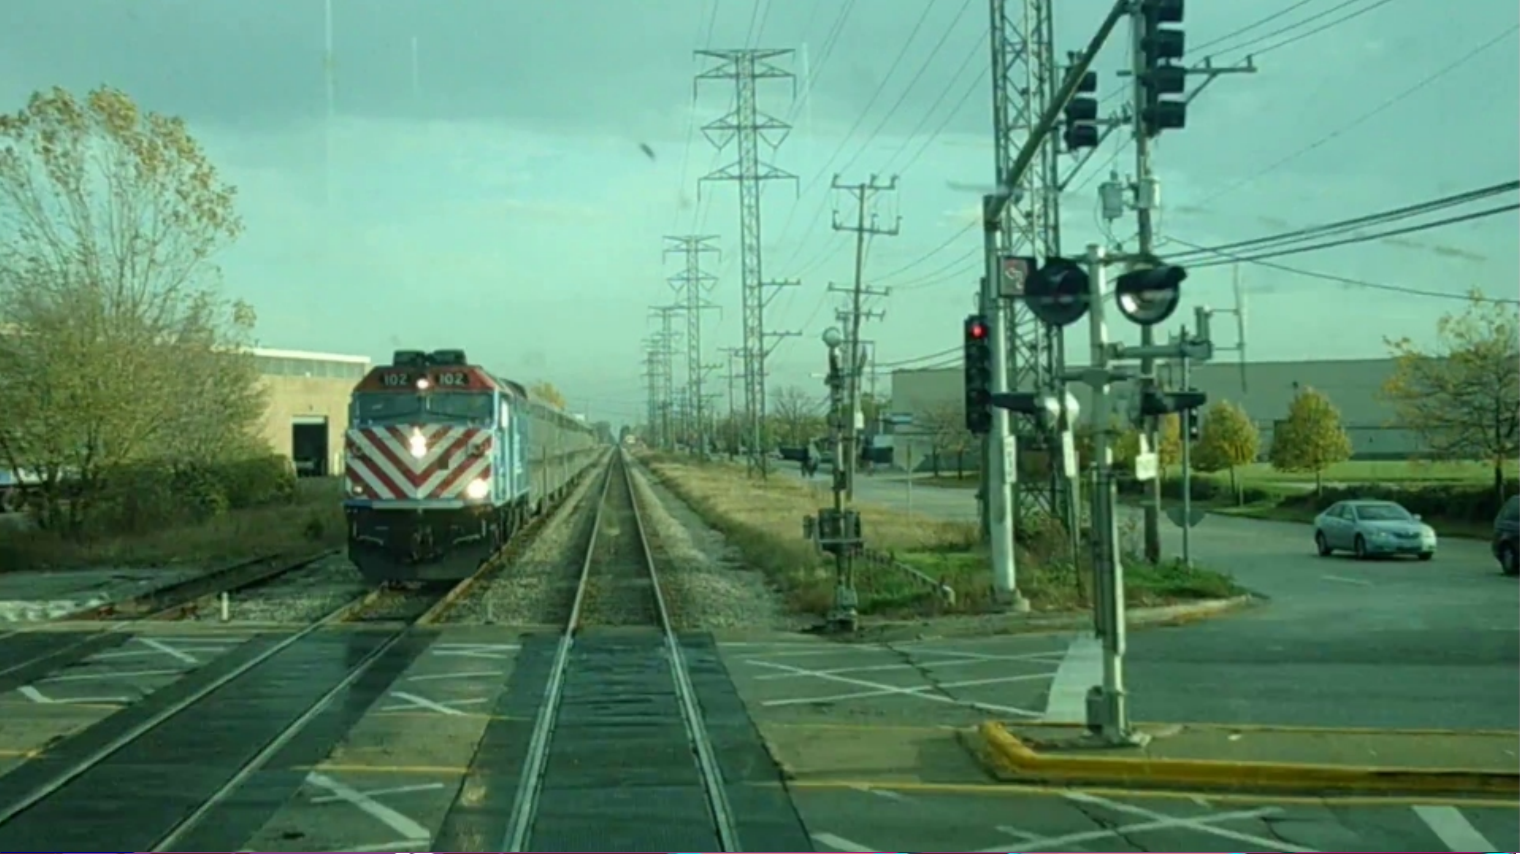
\includegraphics[width=\linewidth]{PICs/datasets/RailSem19_dataset/RailSem19_Bild3.png}
    \end{subfigure}

    \vspace{0.1cm} % Größerer Abstand zwischen den Reihen

    % Zweite Reihe
    \begin{subfigure}{0.328\textwidth}
        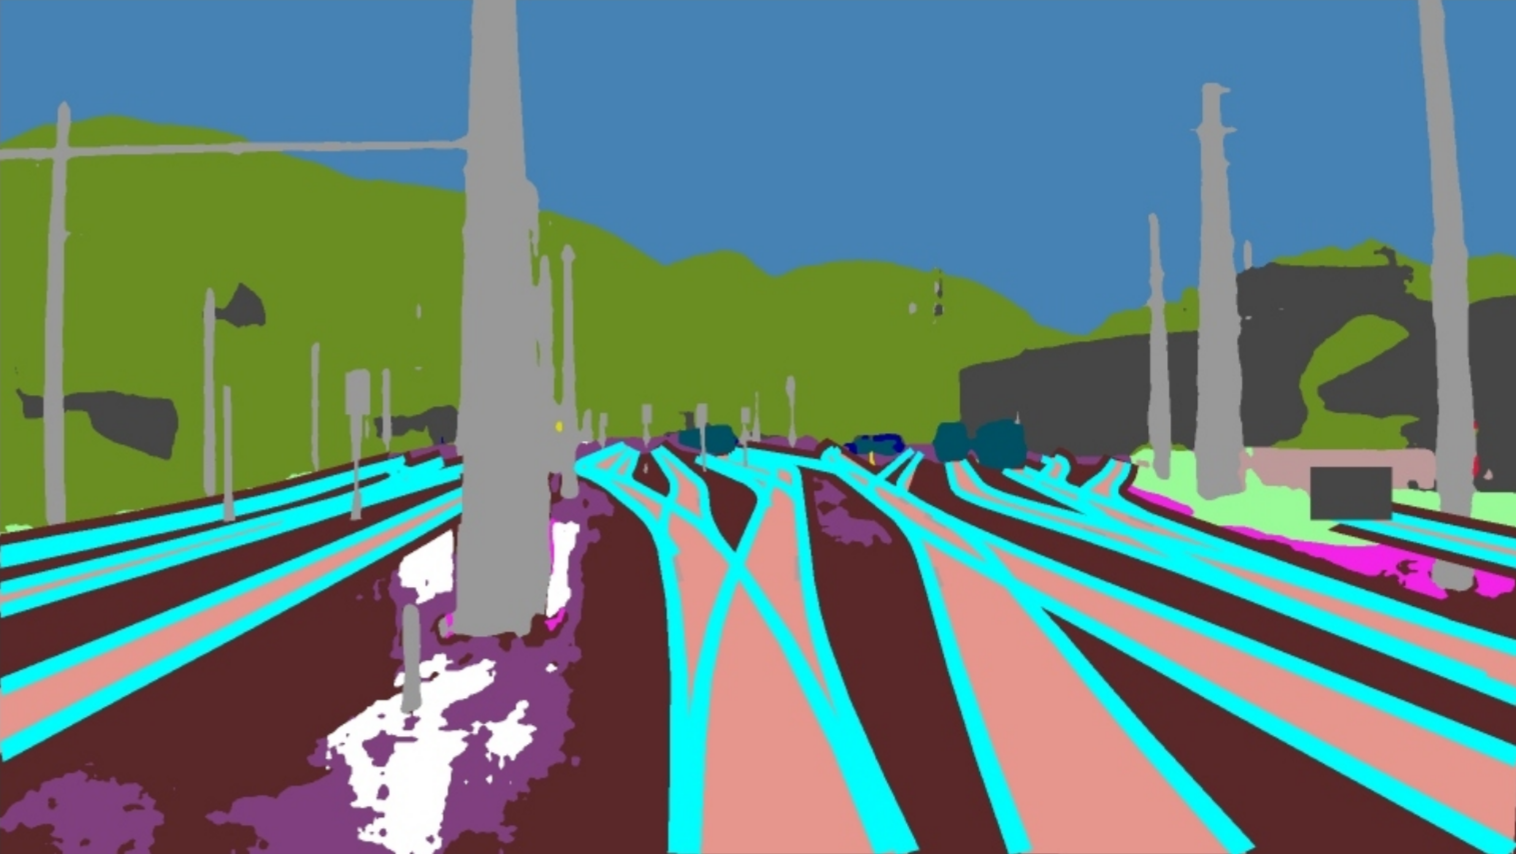
\includegraphics[width=\linewidth]{PICs/datasets/RailSem19_dataset/RailSem19_Bild1_GT.png}
    \end{subfigure}
    \hfill
    \begin{subfigure}{0.328\textwidth}
        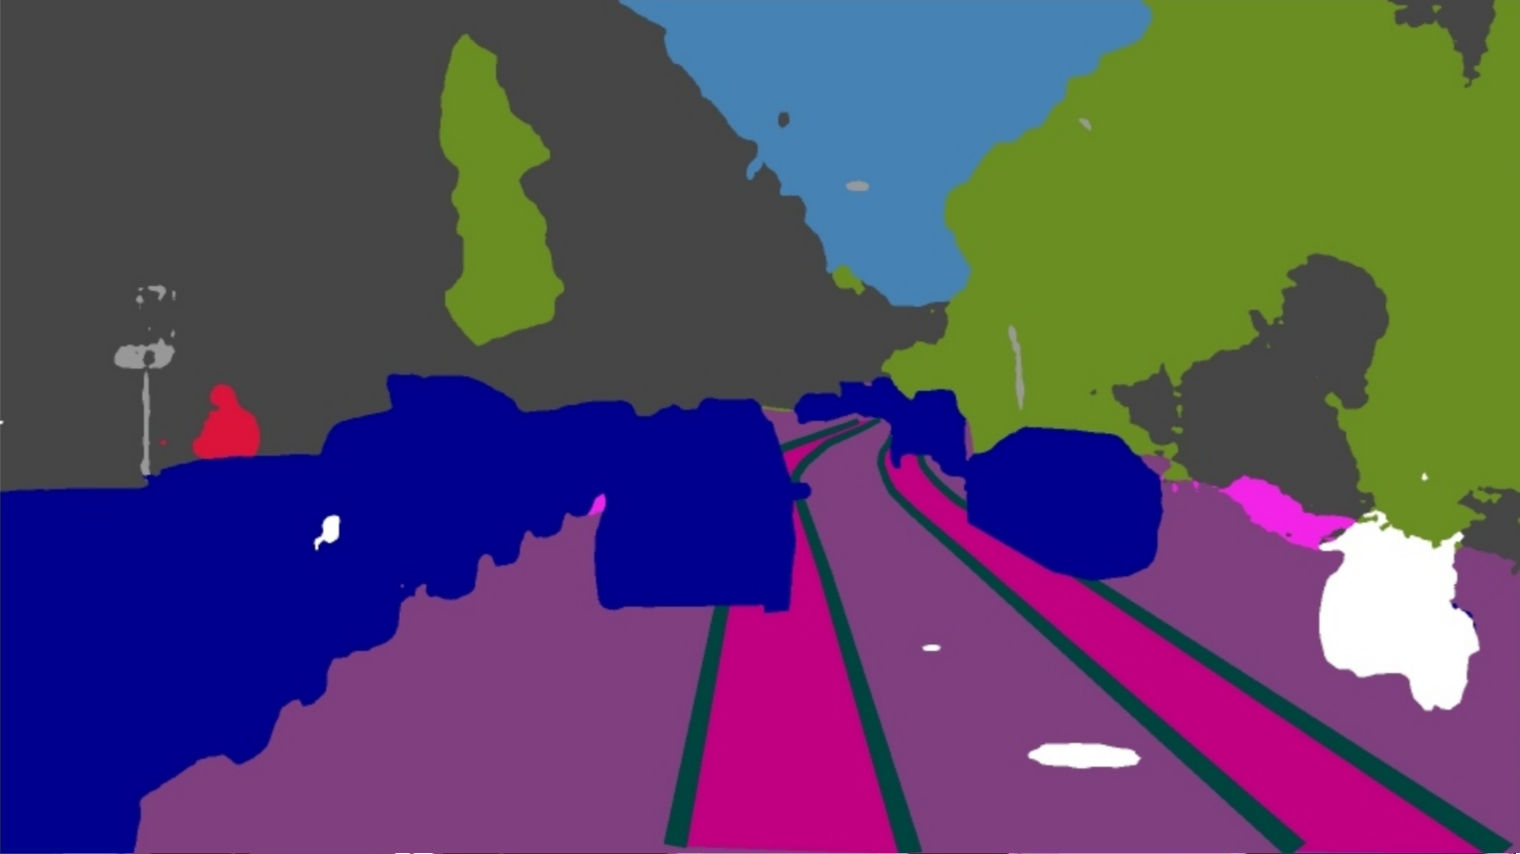
\includegraphics[width=\linewidth]{PICs/datasets/RailSem19_dataset/RailSem19_Bild2_GT.png}
    \end{subfigure}
    \hfill
    \begin{subfigure}{0.328\textwidth}
        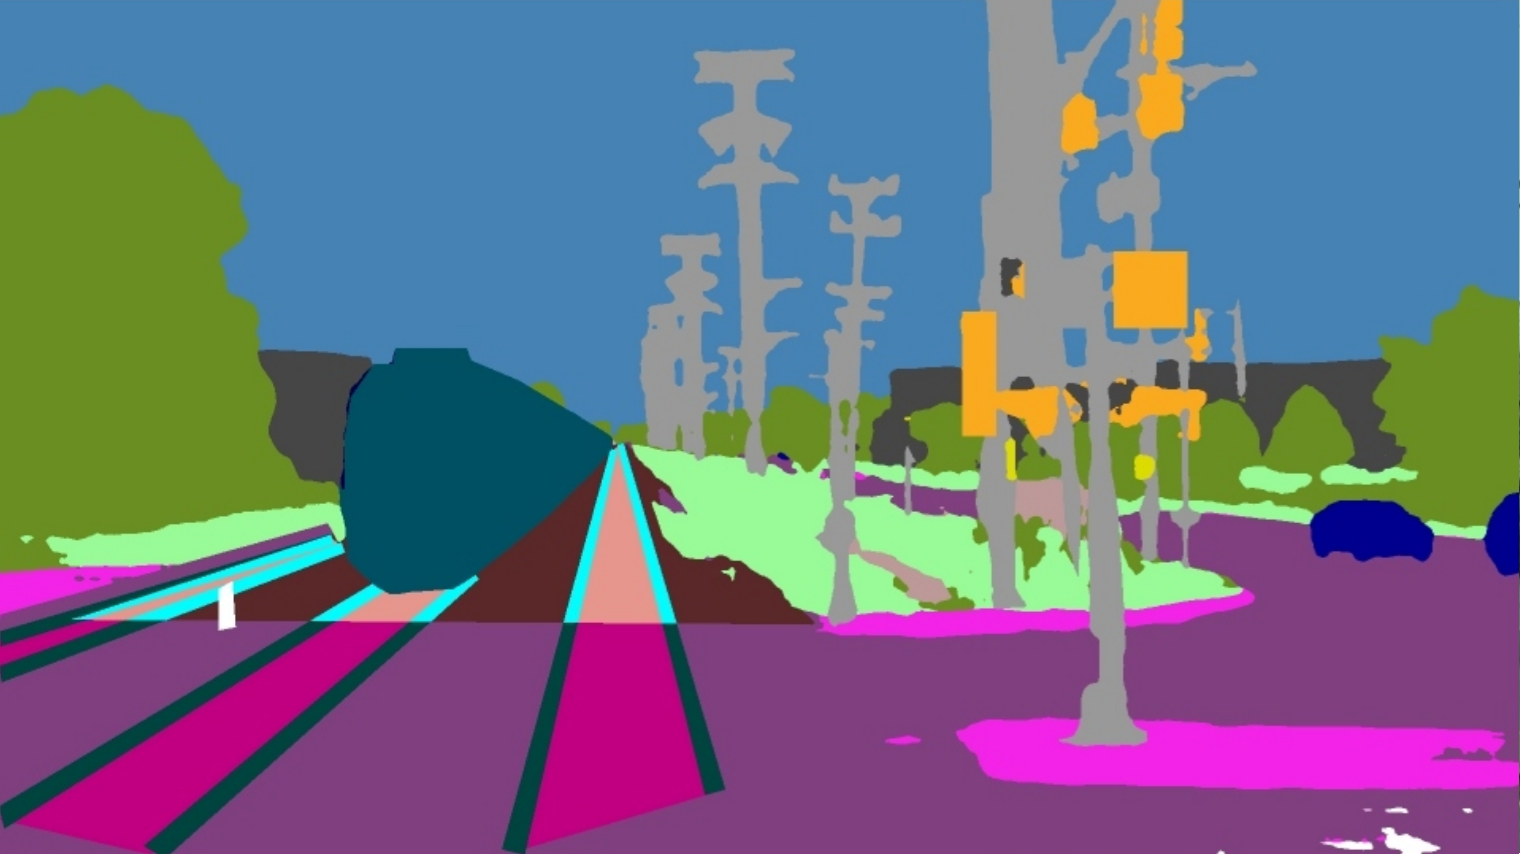
\includegraphics[width=\linewidth]{PICs/datasets/RailSem19_dataset/RailSem19_Bild3_GT.png}
    \end{subfigure}

    \caption{RailSem19 dataset examples. First row raw images. Second row dense \ac{GT} \cite{railsem19dataset}.}
    \label{fig:railSem19-images-denseLabels}
\end{figure}

%RailVID
\subsubsection{RailVID}
\label{subsubsec:railVID}
Another dataset that focuses on the detection of rails is the \textit{RailVID} dataset \cite{yuan2022railvid}. The goal of this project is to detect rail tracks and obstacles on the rails, which can lead to possible hazardous situations. With a functioning system, fully automatic train operation is aimed for. The \textit{RailVID} dataset is a collection of 1071 images with the following labels: \textit{background, railway, car, people}. Since, the area of application is on the "Suzhou Rail Transit Line 1" in Jiangsu Province, China all data is captured there. \textit{RailVID} is a collection of infrared data captured with the AT615X infrared thermal instrument from InfiRay. The decision to use infrared data and not RGB images is because it is more robust against challenging imaging conditions, like darkness at night, fog, rain and direct light disturbance.
Since, this dataset only consists of infrared data and in this work \ac{RGB} data should be used, \textit{RailVID} cannot be used fro training. An additional issue is, that the dataset is recorded only on a specific Chinese line. This is advantageous for this particular use case, but it could become an issue if the system were to be deployed elsewhere.

\begin{figure}[H]
    \centering
    \begin{subfigure}{0.24\textwidth}
        \centering
        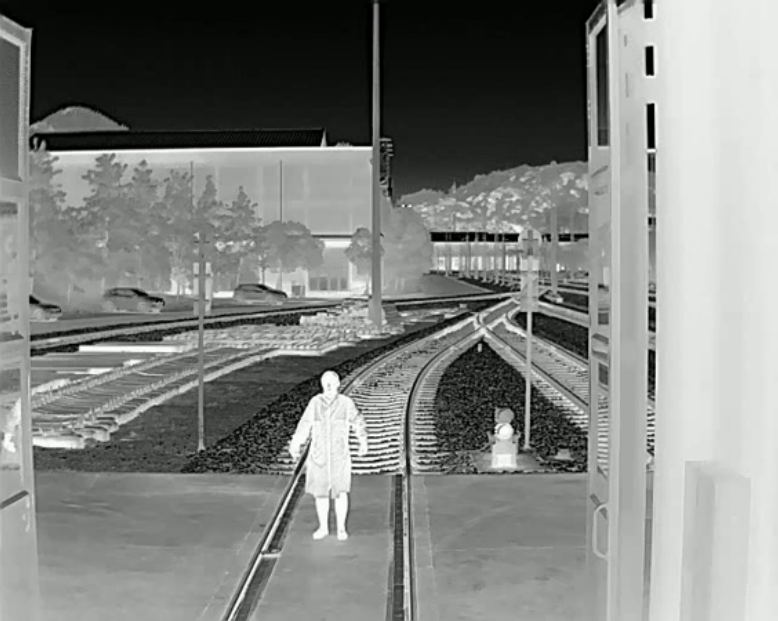
\includegraphics[width=\linewidth]{PICs/datasets/railVID_dataset/railVID_data.png}
    \end{subfigure}
    \hfill
    \begin{subfigure}{0.24\textwidth}
        \centering
        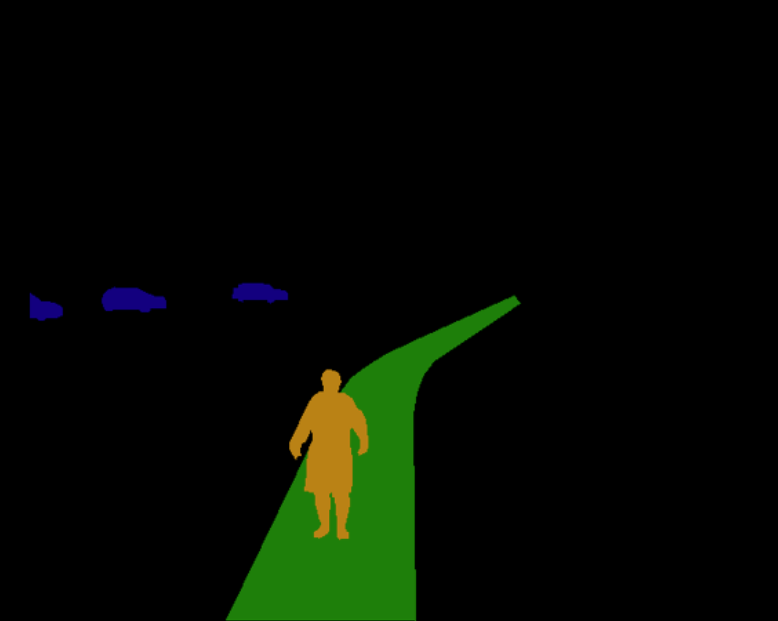
\includegraphics[width=\linewidth]{PICs/datasets/railVID_dataset/railVID_label.png}
    \end{subfigure}
    \hfill
    \begin{subfigure}{0.24\textwidth}
        \centering
        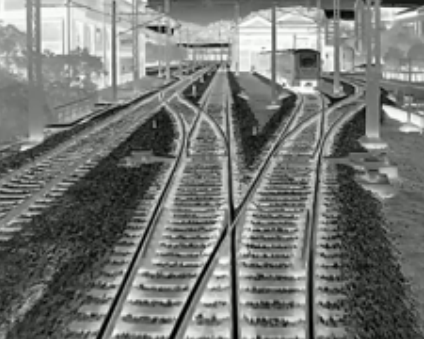
\includegraphics[width=\linewidth]{PICs/datasets/railVID_dataset/railVID_switch.png}
    \end{subfigure}
    \hfill
    \begin{subfigure}{0.24\textwidth}
        \centering
        
\includegraphics[width=\linewidth]{PICs/datasets/railVID_dataset/railVID_switch_label.png}
    \end{subfigure}
    \caption{Example images and \ac{GT} of RailVID dataset \cite{yuan2022railvid}}
    \label{fig:railVID_dataset_images}
\end{figure}

% RailSet
\subsubsection{RailSet}
\cite{railSet2022} and \cite{hadded2022application} presented the \textit{RailSet} dataset,
which is divided into two sub sets: RailSet-Seg for segmentation and RailSet-Ano for anomaly detection \cite{railSet2022}.
Both of them are captured in the ego perspective of the train driver \cite{railSet2022} \cite{hadded2022application}.
The idea is to firstly detect the railways using semantic segmentation and secondly using positional information of the prediction for the creation of the anomaly dataset \cite{railSet2022}.
RailSet-Ano is a collection of 1100 images of railway defects like rail discontinuity and holes in the rail bed.
Some anomalies are taken from a other images and pasted on images of RailSet-Seg and RailSem19 dataset others are generated with a network \cite{railSet2022}.
Since, RailSet-Ano deals with a different use case than the one in this work, this particular data cannot be used.

On the other hand, RailSet-Seg fits the problem. It consists of 6600 images of normal situations.
The images are collected from 23 YouTube videos with a collective duration of 15 hours. It includes two labels: \textit{rail} and \textit{rail-track}.
Besides the use of  RailSet-Seg for the creation of RailSet-Ano, an additional motivation is to include more complex scenes of the rail domain than RailSem19.
That is why the focus of RailSet lies on scenarios with poor weather conditions or lighting conditions.
Furthermore, images are included in which the rails are not visible at all, like in tunnels without lighting or in snowy scenes.
Additionally, it was ensured that the videos were recorded by different cameras and from different mounting positions \cite{railSet2022} \cite{hadded2022application}. 

An advantage of this dataset is that it can be joined with RailSem19, when combining four specific labels.
\textit{trackbed} and \textit{rail-track} from RailSem19 have to be transformed into RailSet's \textit{rail-track} label and \textit{rail-raised} and \textit{rail-embedded} become the \textit{rail} label.
This method leads to more data for the training and validation which could be an advantage.
However, it also shows the disadvantage of this dataset for the specific use case of this work. 
RailSet exclusively addresses railway and not tram scenes \cite{hadded2022application}.
Since, the goal is to target a broad applicability, leaning towards tram scenes this dataset is not used for this work.

% Bild von RailSet
\begin{figure}[H]
    \centering
    \begin{subfigure}{0.3\textwidth}
        \centering
        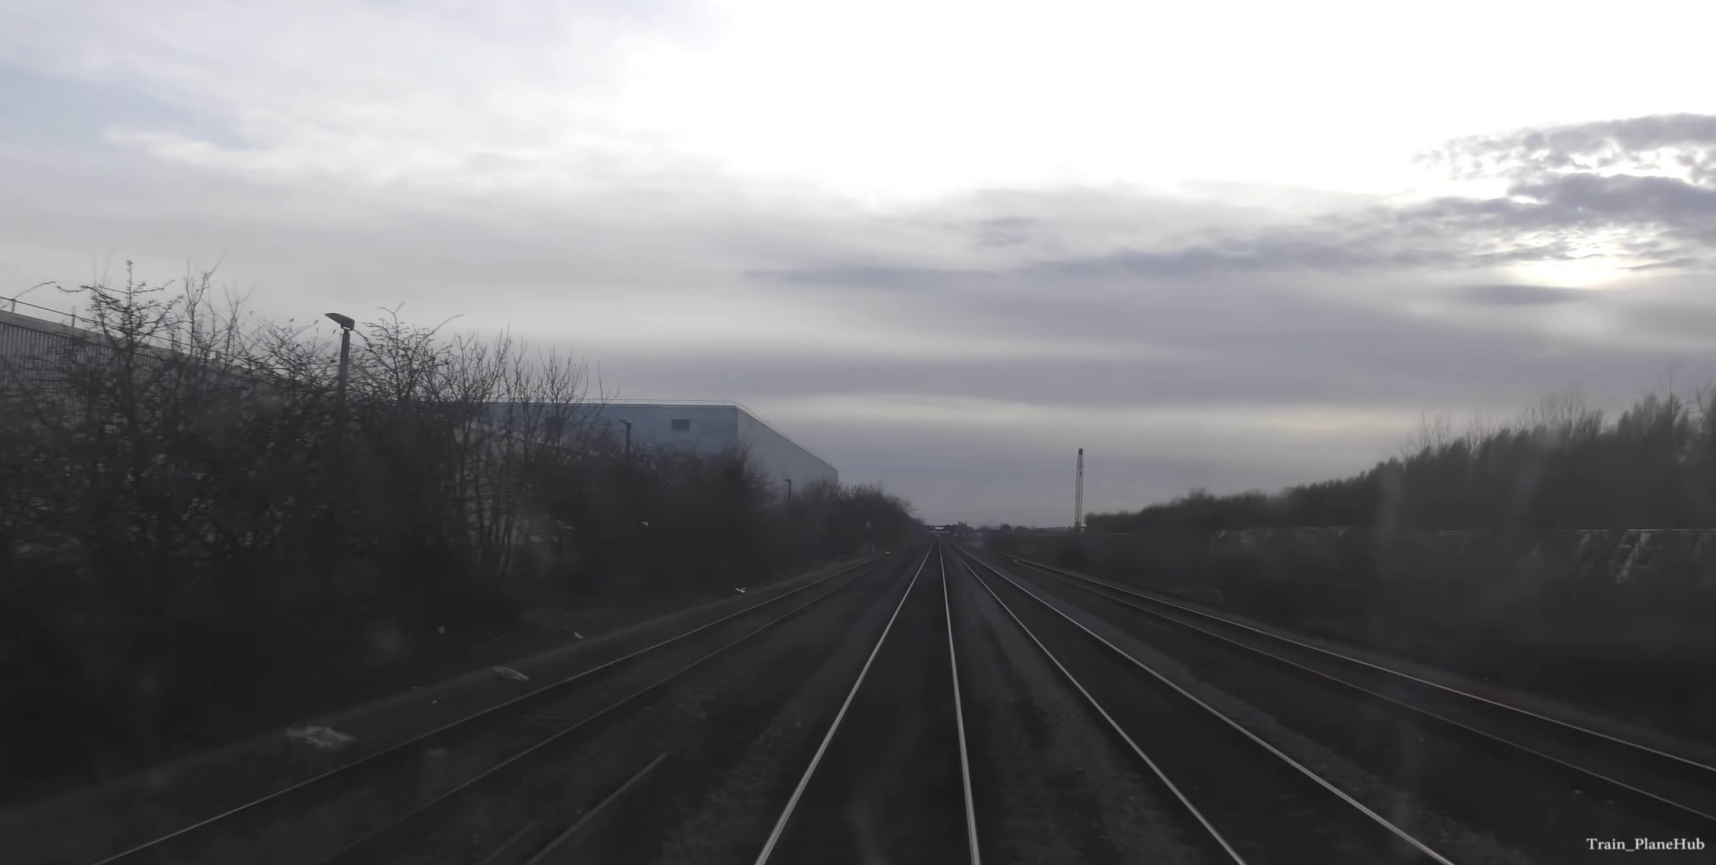
\includegraphics[width=\linewidth,height=5cm,keepaspectratio]{PICs/datasets/RailSet_dataset/RailSet_image.png}
        \caption{}
        \label{fig:RailSet-Seg_example_image_GT_a}
    \end{subfigure}
    \hspace*{0.02\textwidth} % Abstand manuell steuern
    \begin{subfigure}{0.3\textwidth}
        \centering
        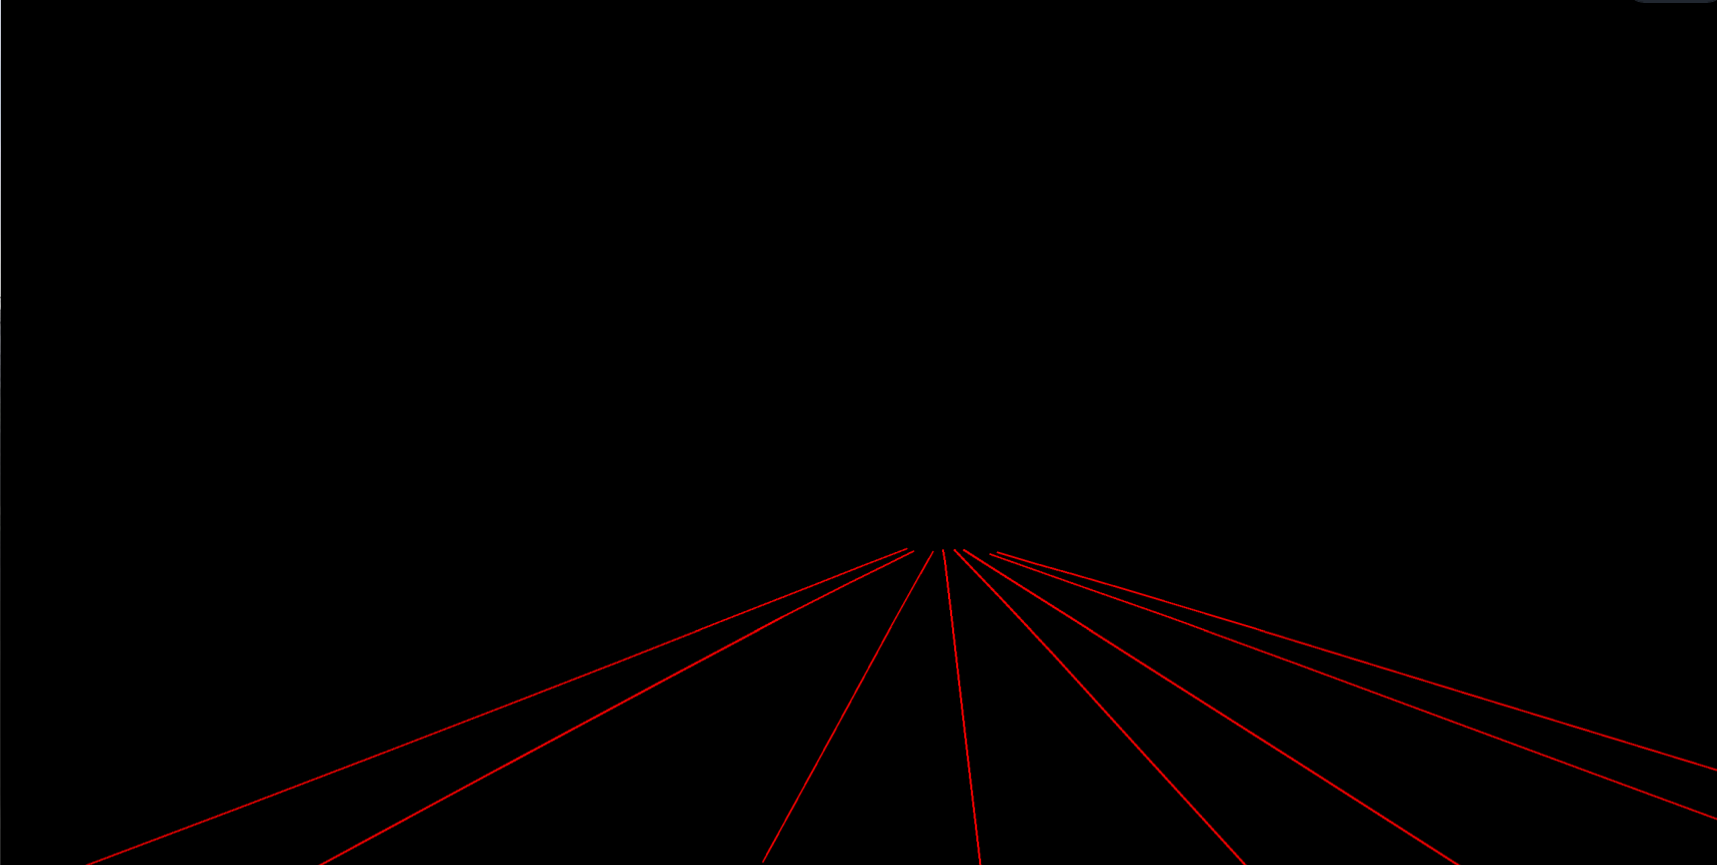
\includegraphics[width=\linewidth,height=5cm,keepaspectratio]{PICs/datasets/RailSet_dataset/RailSet_GT_rails.png}
        \caption{}
        \label{fig:RailSet-Seg_example_image_GT_b}
    \end{subfigure}
    \hspace*{0.02\textwidth} % Abstand manuell steuern
    \begin{subfigure}{0.3\textwidth}
        \centering
        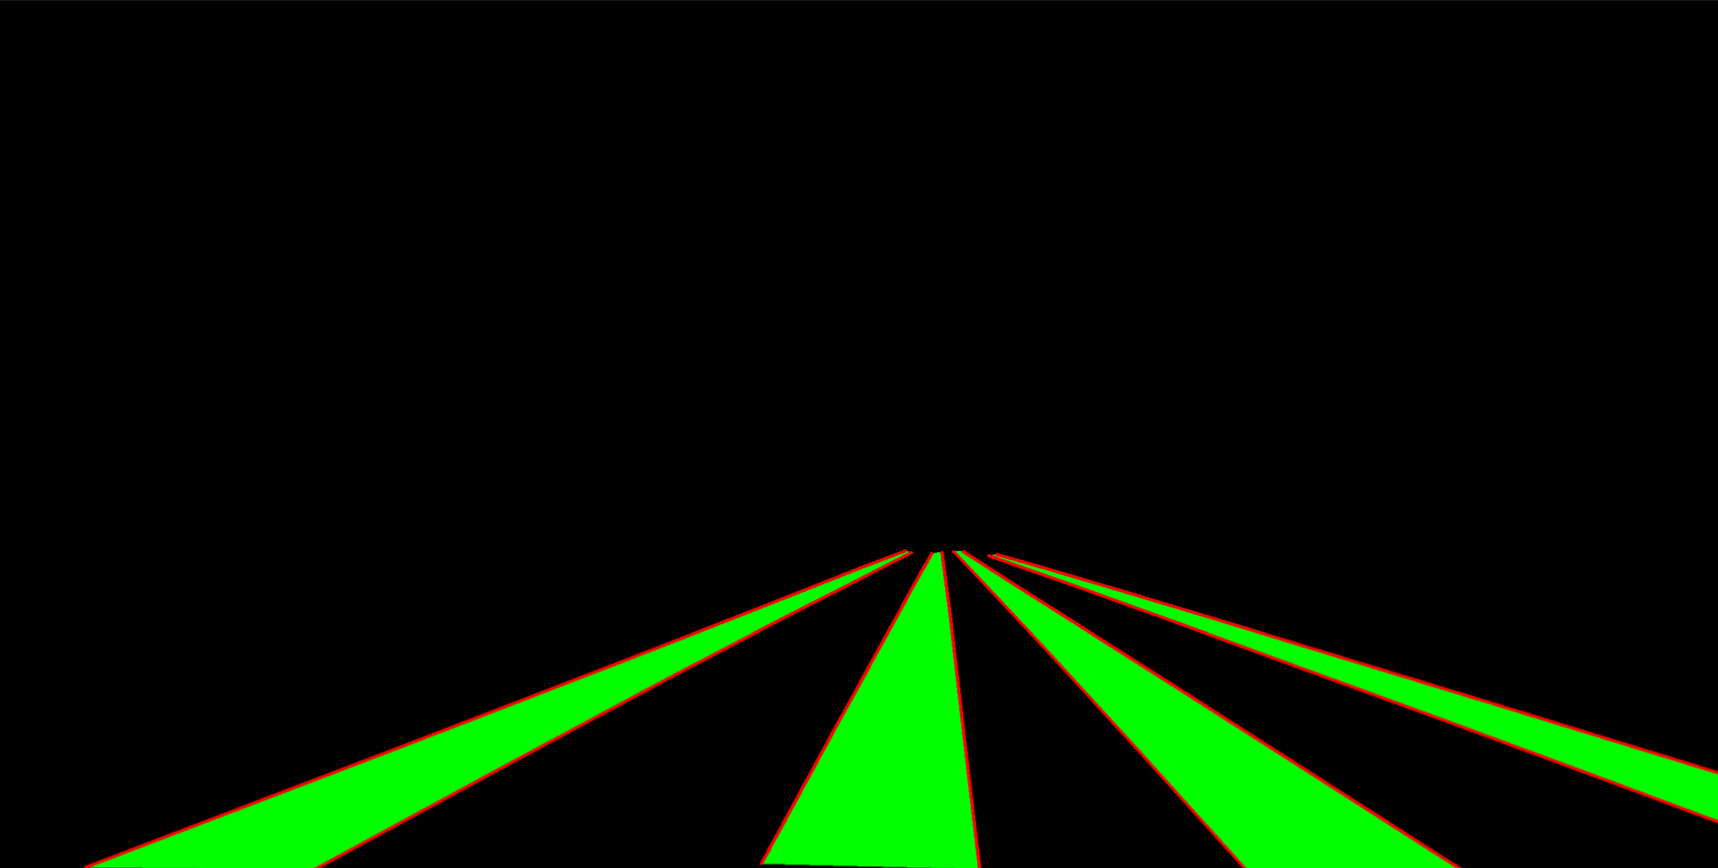
\includegraphics[width=\linewidth,height=5cm,keepaspectratio]{PICs/datasets/RailSet_dataset/RailSet_GT_rails&rail-track.png}
        \caption{}
        \label{fig:RailSet-Seg_example_image_GT_c}
    \end{subfigure}
    \caption{RailSet-Seg example with annotations \cite{railSet2022} \cite{hadded2022application}: \textbf{(a)} raw-image, \textbf{(b)} rail class, \textbf{(c)} rail and rail-track class}
    \label{fig:RailSet-Seg_example_image_GT}
\end{figure}


% RSDS
\subsubsection{RSDS}
The creators of the \ac{RSDS} \cite{railNet2019}, tried to solve the railroad detection problem with a segmentation approach. Because there was no publicly available dataset for this task at the time, they had to construct their own. \ac{RSDS} is captured from the ego perspective of the train driver and is a collection of 3000 images. They used 2500 for training, 200 for validation and 300 for testing. The dataset only includes one \textit{railroad} label. It is described that the labels only incorporate pixels between the two rails and intentionally ignore railway sleepers outside this area. Images are of size 1920 x 1080.
Although it is not mentioned in the paper, it seems as if all images of \ac{RSDS} are captured from a specific rail line in China. Additionally, from the images in the paper alone one can tell that this particular rail line has very distinctive structural characteristics. The colors are bright and it seems like the area between the rails is mostly concrete, which is unusual for most railways. \ref{fig:RSDS_example_image_GT} shows that structures besides the rails are specific too.
One additional detail of this dataset, which can present a disadvantage for this work, is that switches are not addressed.
Since this dataset only covers very specific railroads with unique characteristics and additionally does not address switches or other situations where the track splits, \ac{RSDS} is not further considered for this work.

% Bild von RSDS
\begin{figure}[H]
    \centering
    \begin{subfigure}{0.45\textwidth}
        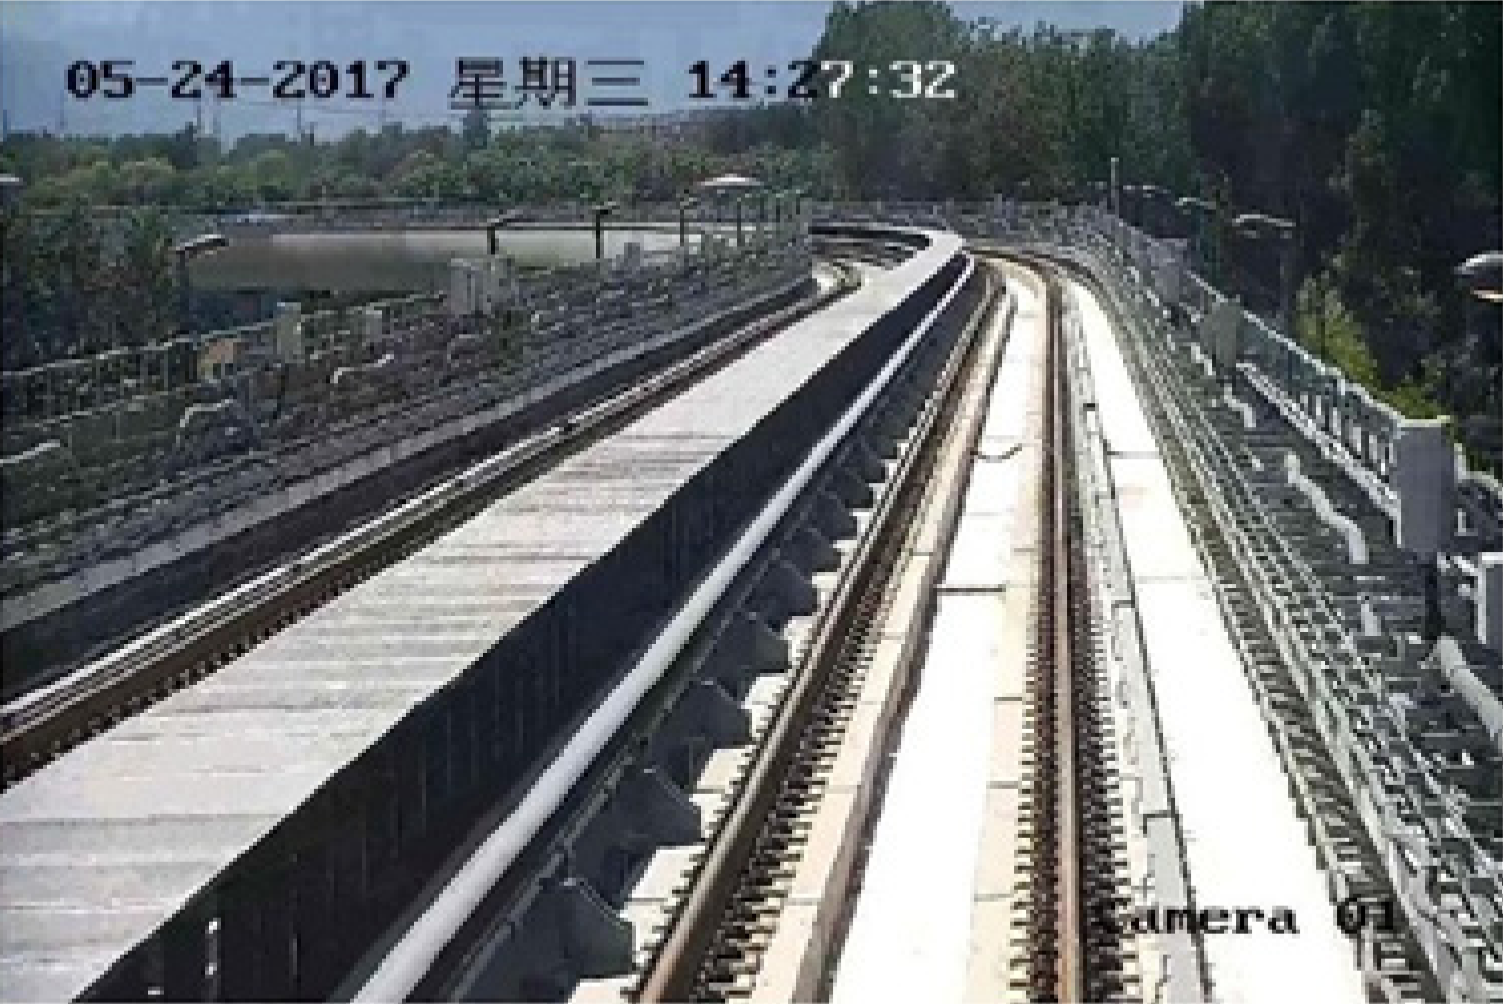
\includegraphics[width=\linewidth,height=5cm,keepaspectratio]{PICs/datasets/RSDS_dataset/RSDS_image.png}
        \caption{}
        \label{fig:RSDS_example_image_GT_a}
    \end{subfigure}
    \hfill
    \begin{subfigure}{0.45\textwidth}
        
\includegraphics[width=\linewidth,height=5cm,keepaspectratio]{PICs/datasets/RSDS_dataset/RSDS_GT.png}
        \caption{}
        \label{fig:RSDS_example_image_GT_b}
    \end{subfigure}
    \caption{\ac{RSDS} example with annotation \cite{railNet2019}: \textbf{(a)} raw-image, \textbf{(b)} ground truth}
    \label{fig:RSDS_example_image_GT}
\end{figure}

% Rail-DB
\subsubsection{Rail-DB}
A very similar dataset is Rail-DB \cite{li2022rail}.
This dataset is a collection of 7432 images, which are taken from 15 videos.
The labels in this dataset are consist of poly lines, which represent all existing rails in an image.
Additionally the the poly lines all have different classes. This way there is not only one rail class, but as many classes as there are rails in one image.
The labeling policy specifies that the central rails are marked with the annotations 1 and 2.
Additional rails are labeled with rising numbers.
Since this dataset includes poly lines and not binary masks, this dataset can be used for training line detection algorithms.
Compared to \ac{RSDS}, this dataset includes not only lines and curves, but also rail switches.
Additionally, the images are taken in various conditions and scenes.
\ref{fig:Rail-DB-dataset_images_annotated} shows example images of Rail-DB's different scenes.
However, it seems that the images again have very specific characteristics like in \ac{RSDS}.
\ref{fig:Rail-DB-dataset_images_annotated} also shows, that all images are captured on a Chinese line.
Even though \cite{li2022rail} presents a very interesting approach for solving the rail detection problem,
because of the before mentioned specific characteristics it is not used for this work. Even the author of \cite{li2022rail} states in the GitHub repository \cite{railNet2022GitHub},
that this project fails to generalize on example videos, where the scene looks different from the one the dataset is captured on.

\begin{figure}[H]
    \centering
    \begin{subfigure}{0.328\textwidth}
        \centering
        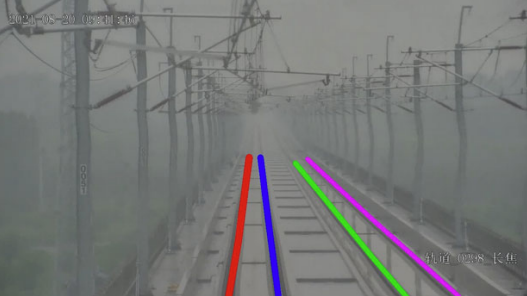
\includegraphics[width=\linewidth,height=5cm,keepaspectratio]{PICs/datasets/railDB_dataset/railDB_fog.png}
    \end{subfigure}
    %\hspace*{0.02\textwidth} % Abstand manuell steuern
    \hfill
    \begin{subfigure}{0.328\textwidth}
        \centering
        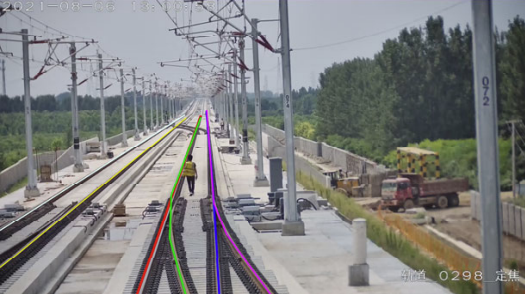
\includegraphics[width=\linewidth,height=5cm,keepaspectratio]{PICs/datasets/railDB_dataset/railDB_switch.png}
    \end{subfigure}
    %\hspace*{0.02\textwidth} % Abstand manuell steuern
    \hfill
    \begin{subfigure}{0.328\textwidth}
        \centering
        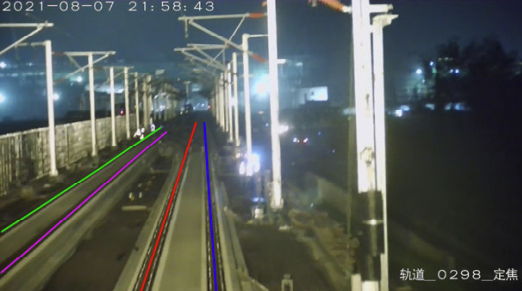
\includegraphics[width=\linewidth,height=5cm,keepaspectratio]{PICs/datasets/railDB_dataset/railDB_night.png}
    \end{subfigure}
    \caption{Rail-DB \cite{li2022rail} images with annotations in different conditions}
    \label{fig:Rail-DB-dataset_images_annotated}
\end{figure}


% OSDaR23
\subsubsection{OSDaR23}
Another dataset it the OSDaR23 \cite{oSDaR23}.
This dataset is a collection of 21 sequences, which are split into 45 subsequences.
Several sequences are short ones with 10 frames each, some are longer with 40 to 100 frames.
In total there are 1534 labeled scenes in this dataset.
Since, OSDaR23 is captured with 9 cameras (\ac{RGB} and \ac{IR}) in different angles, one lidar and one radar sensor, the total number of frames are 1534 * 11 = 16874.
Additionally, position and acceleration sensors are used.
Because also lidar and radar is used, this dataset offers 3D data as well.
OSDaR23 consists of 20 different labels.
These labels include the rail context, like \textit{track}, \textit{switch} or \textit{train} and the environment, like \textit{person}, \textit{animal}, \textit{bicycle}, \textit{smoke}, \textit{flame} or \textit{crowd}.
The annotations for the environment can be used for safety applications.
For more details please refer to \textit{TABLE V} in \cite{oSDaR23}.
\ref{fig:OSDaR23_captured_data} shows the 11 different frames of each sensor and \ref{fig:OSDaR23_annotated} shows an example of an annotated scene.
As illustrated in \ref{fig:OSDaR23_annotated} the \textit{track} label and the \textit{switch} label only offers positional information about their presents, but do not include any information on the direction of the train.
Furthermore, there is no information that distinguishes the train rails from the adjacent rails.
Therefore OSDaR23 can only be used for the detection of rails, but not the track prediction.
Moreover, the capturing of this dataset only took place on rail roads in Hamburg, Germany.
No tram scenes are included.
Due to the necessity of re-labeling for this work and the fact that only data from Hamburg is offered, OSDaR23 is not used.


% captured data
\begin{figure}[H]
    \centering
    % Erstes Bild
    \begin{subfigure}{\textwidth}
        \centering
        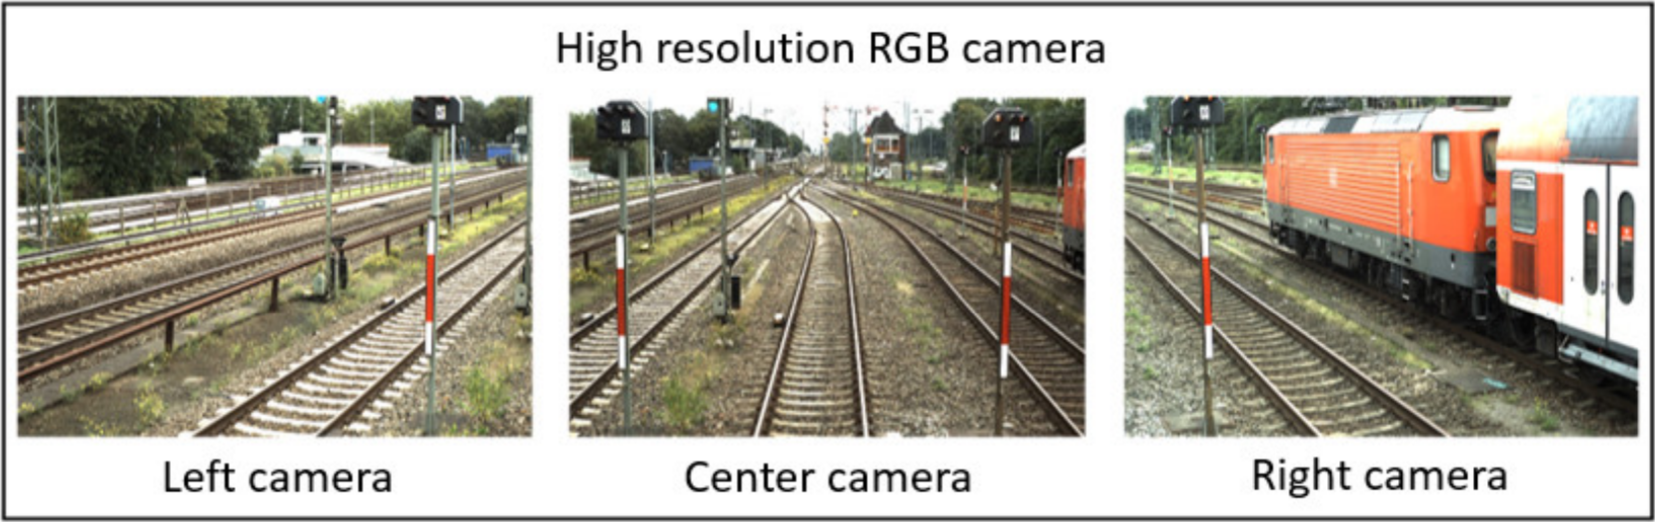
\includegraphics[width=0.5\textwidth]{PICs/datasets/OSDaR23_dataset/camerasetup_high_res_cameras.png}
    \end{subfigure}

    % Zweites Bild
    \begin{subfigure}{\textwidth}
        \centering
        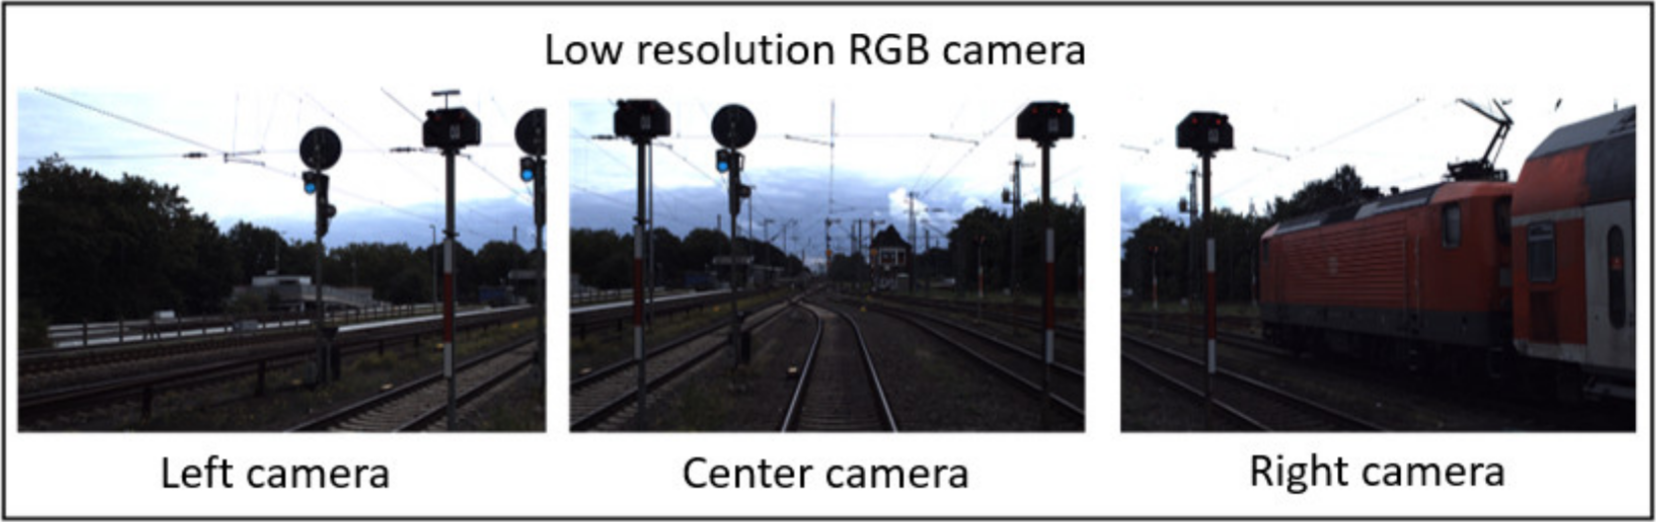
\includegraphics[width=0.5\textwidth]{PICs/datasets/OSDaR23_dataset/camerasetup_low_res_cameras.png}
    \end{subfigure}

    % Drittes Bild
    \begin{subfigure}{\textwidth}
        \centering
        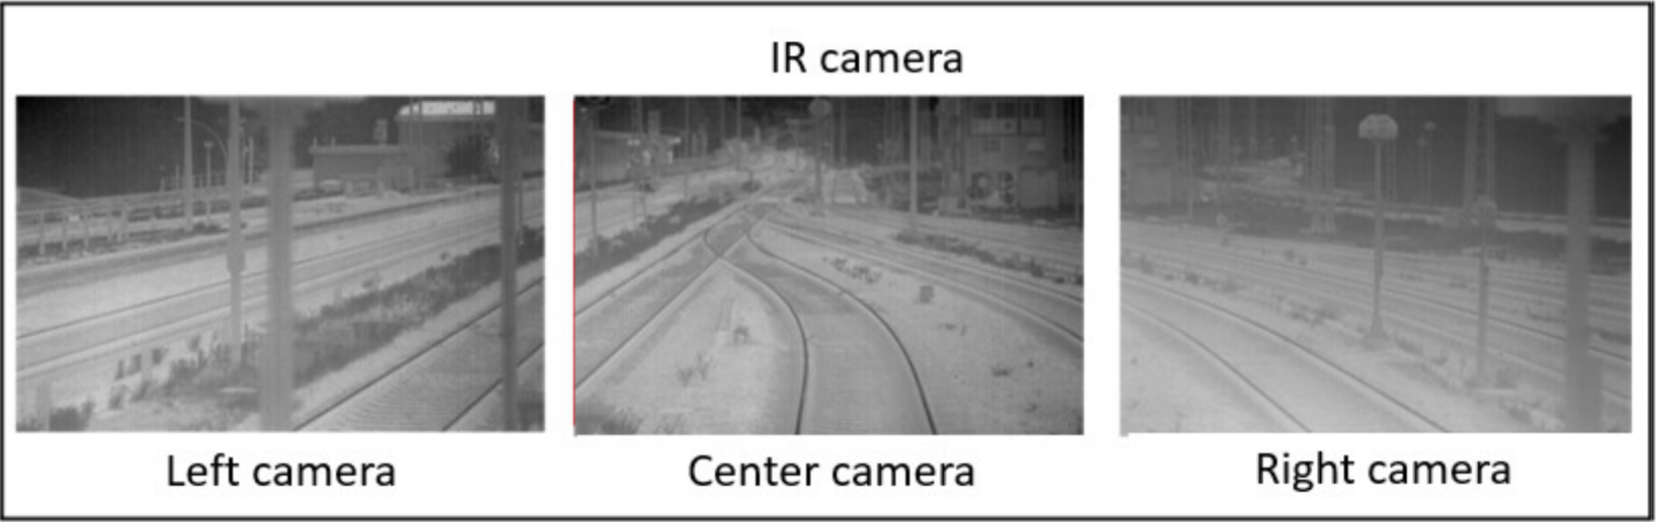
\includegraphics[width=0.5\textwidth]{PICs/datasets/OSDaR23_dataset/camerasetup_IR.png}
    \end{subfigure}

    % Viertes Bild
    \begin{subfigure}{\textwidth}
        \centering
        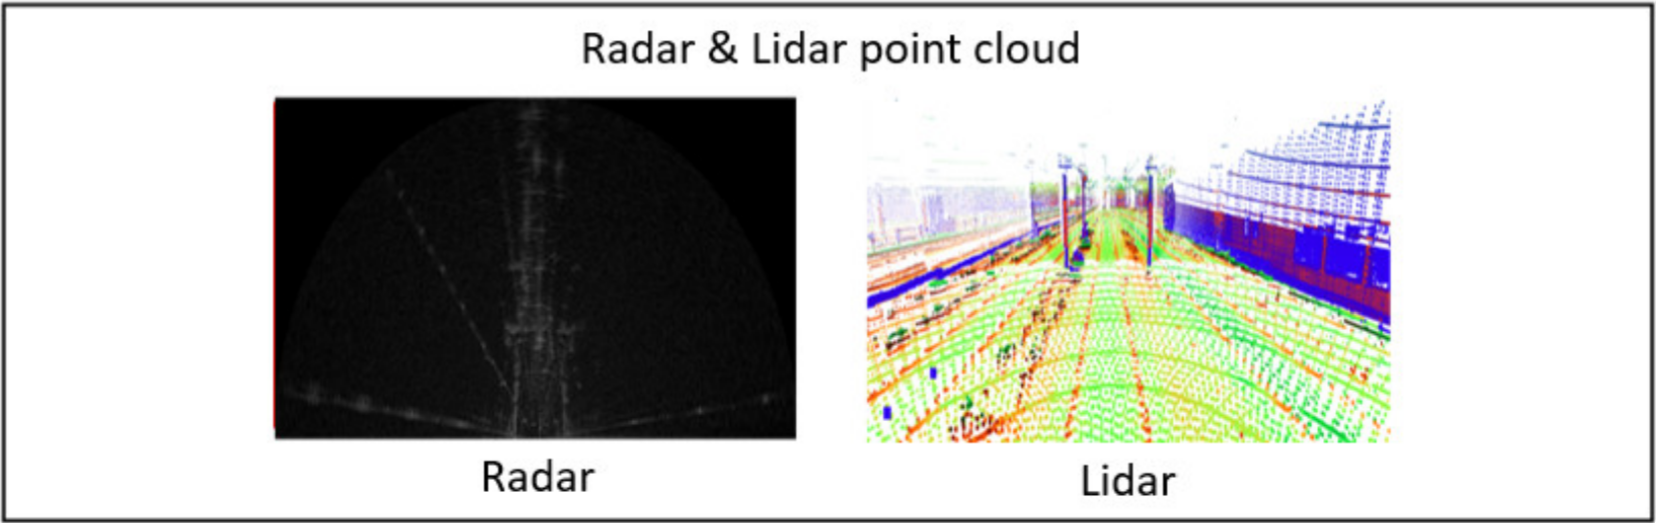
\includegraphics[width=0.5\textwidth]{PICs/datasets/OSDaR23_dataset/camerasetup_Lidar_Radar.png}
    \end{subfigure}
    
    \caption{OSDaR23 data from all different sensors \cite{oSDaR23}}
    \label{fig:OSDaR23_captured_data}
\end{figure}

% labeled scene
\begin{figure}[H]
    \centering
    % Erste Reihe: Zwei Bilder nebeneinander
    \begin{subfigure}{0.45\textwidth}
        \centering
        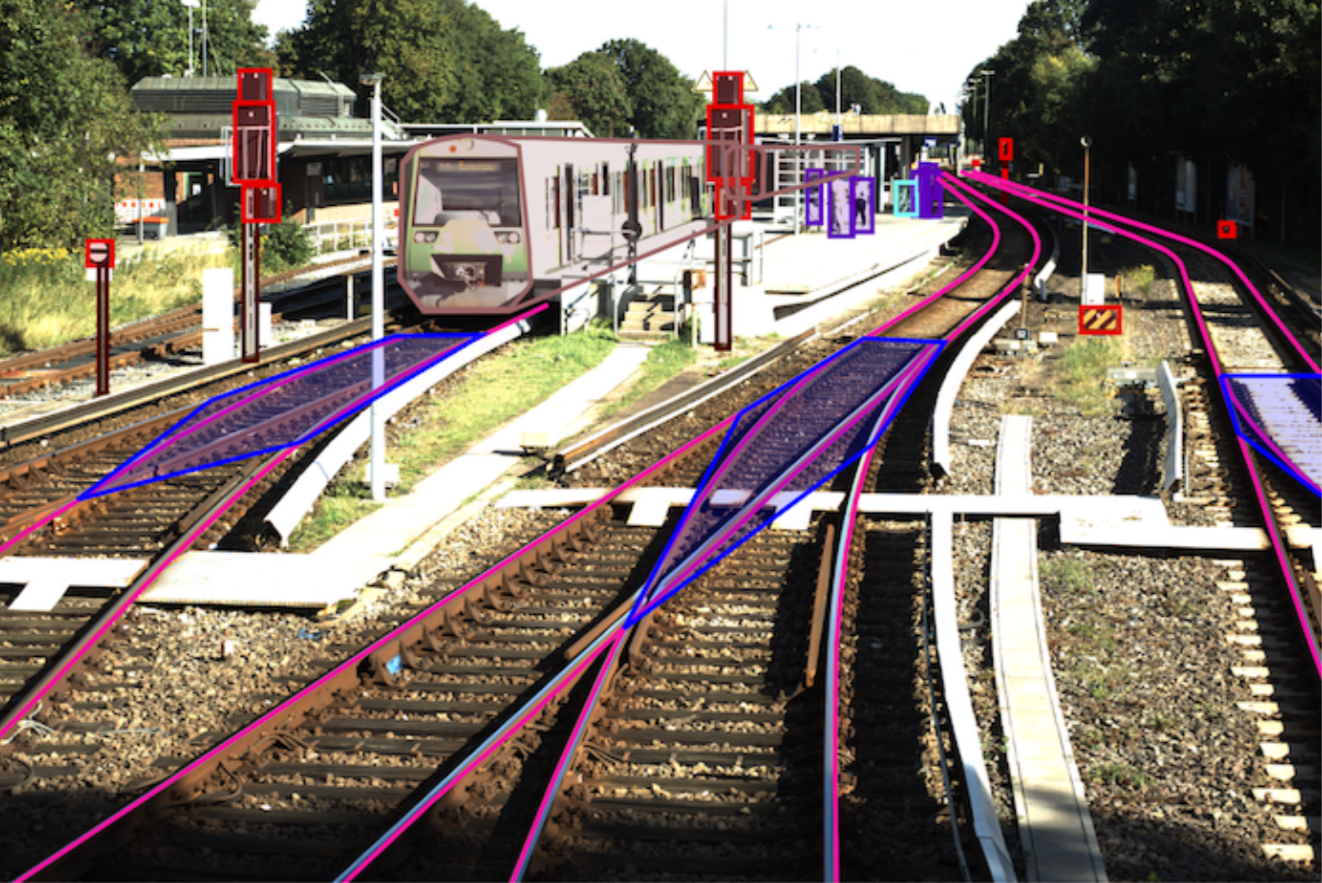
\includegraphics[width=\textwidth]{PICs/datasets/OSDaR23_dataset/labeled_image.png}
        \caption{\ac{RGB} center camera}
    \end{subfigure}%
    \hspace{0.05\textwidth}
    \begin{subfigure}{0.45\textwidth}
        \centering
        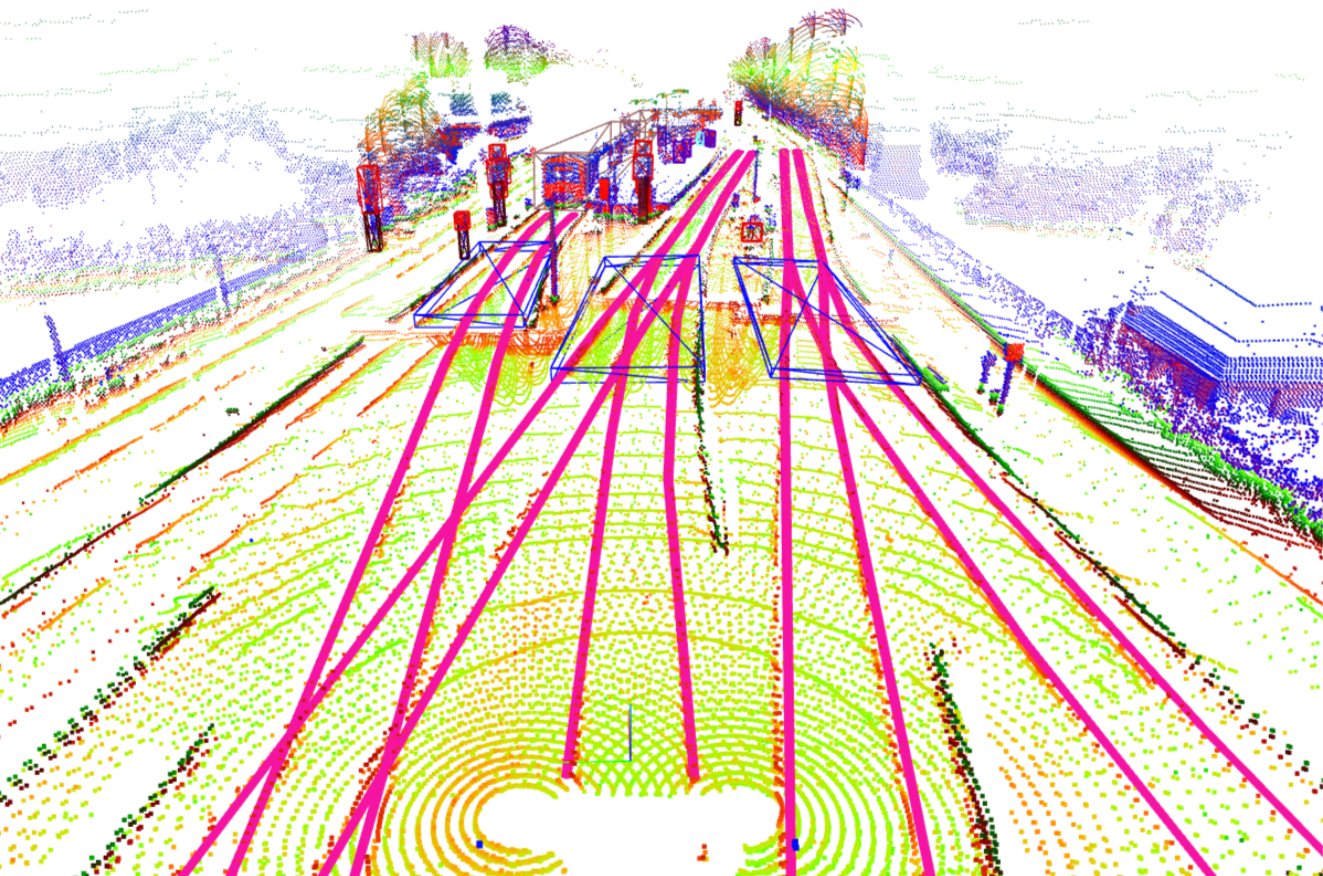
\includegraphics[width=\textwidth]{PICs/datasets/OSDaR23_dataset/labeled_3D.png}
        \caption{merged lidar point cloud}
    \end{subfigure}

    \vspace{0.5cm} % Abstand zwischen den Reihen

    % Zweite Reihe: Zwei Bilder nebeneinander
    \begin{subfigure}{0.45\textwidth}
        \centering
        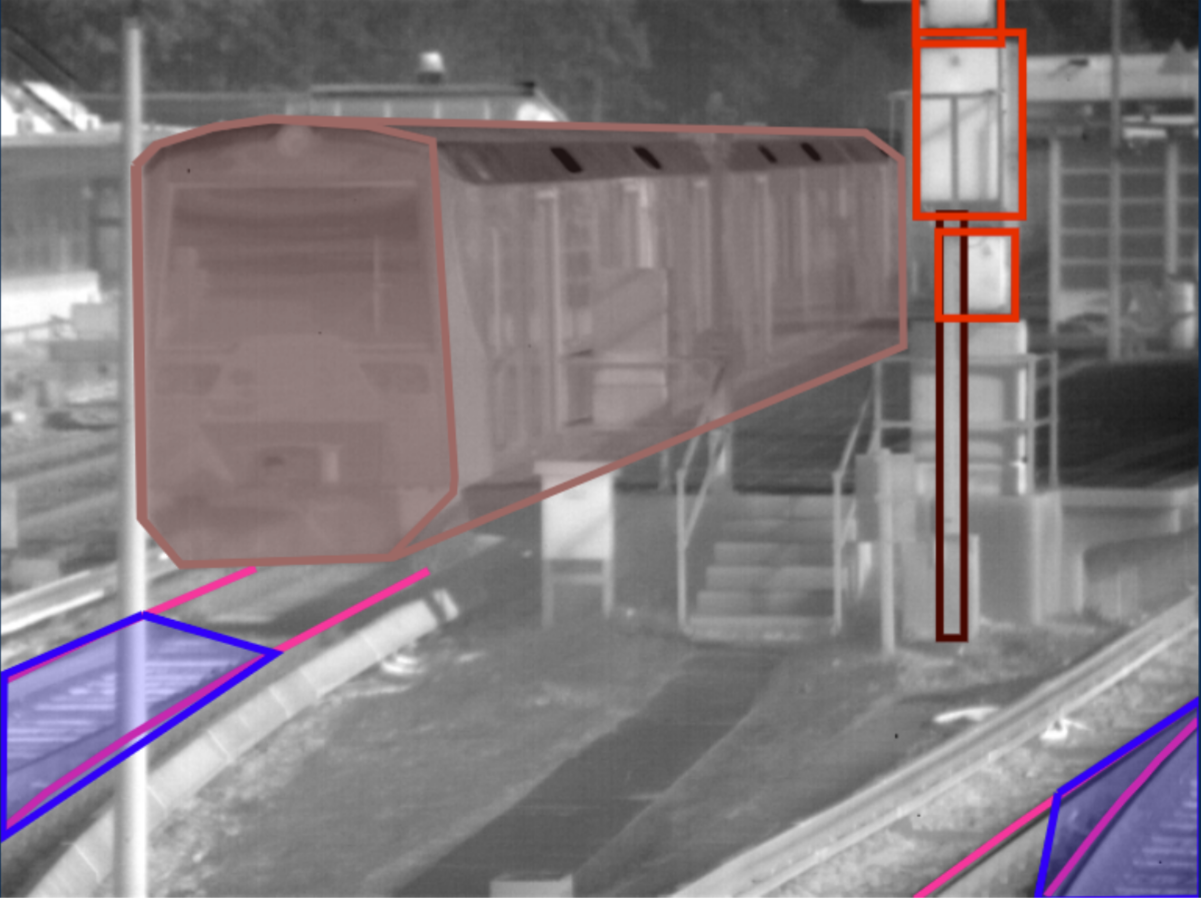
\includegraphics[width=\textwidth]{PICs/datasets/OSDaR23_dataset/labeled_IR.png}
        \caption{IR center camera}
    \end{subfigure}%
    \hspace{0.05\textwidth}
    \begin{subfigure}{0.45\textwidth}
        \centering
        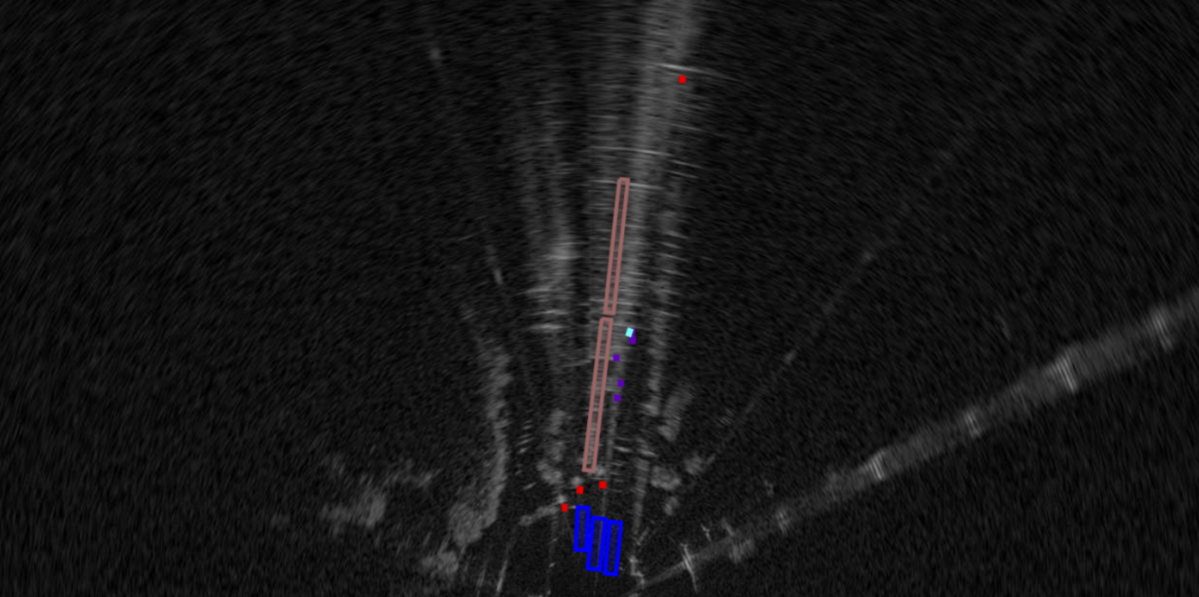
\includegraphics[width=\textwidth]{PICs/datasets/OSDaR23_dataset/labeled_Radar.png}
        \caption{Radar (zoomed)}
    \end{subfigure}
    
    \caption{OSDaR23 annotated scene \cite{oSDaR23}}
    \label{fig:OSDaR23_annotated}
\end{figure}



\begin{figure}[H]
    \centering
    % Erste Reihe: Zwei Bilder nebeneinander, feste Breite und Höhe
    \begin{subfigure}{0.45\textwidth}
        \centering
        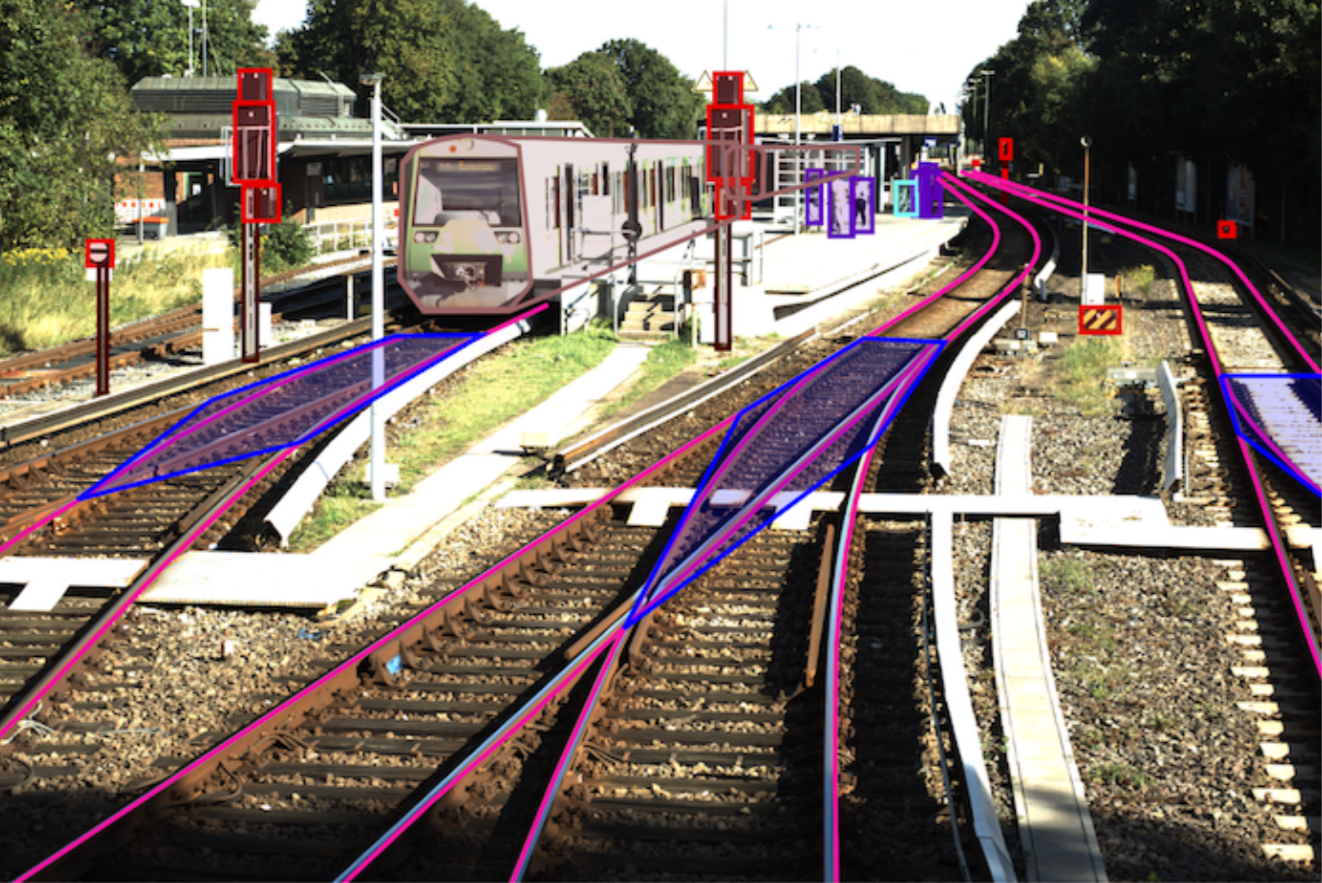
\includegraphics[width=0.9\textwidth,height=5cm]{PICs/datasets/OSDaR23_dataset/labeled_image.png}
        \caption{Bild 1}
    \end{subfigure}%
    \hspace{0.05\textwidth}
    \begin{subfigure}{0.45\textwidth}
        \centering
        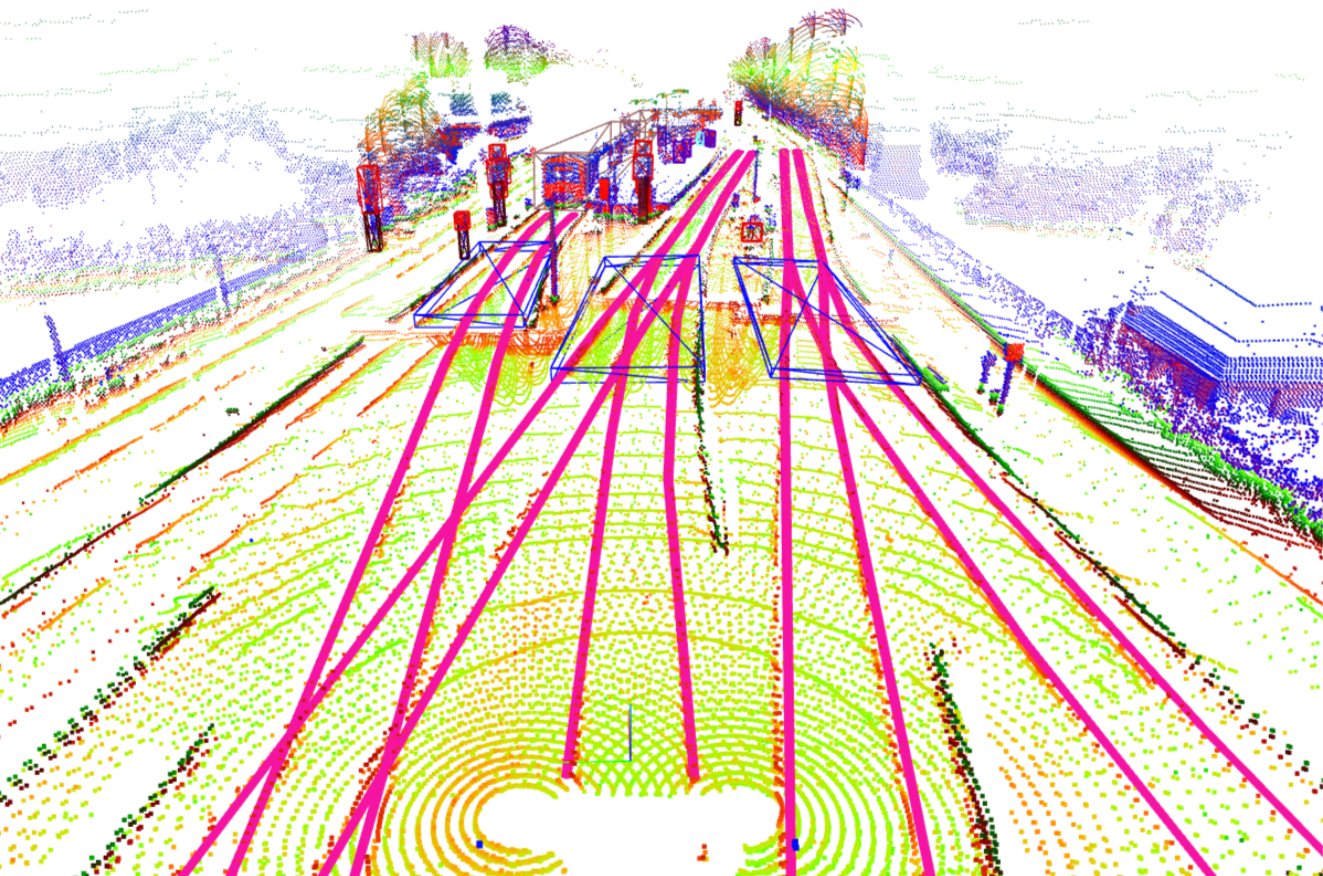
\includegraphics[width=0.9\textwidth,height=5cm]{PICs/datasets/OSDaR23_dataset/labeled_3D.png}
        \caption{Bild 2}
    \end{subfigure}

    \vspace{0.5cm} % Abstand zwischen den Reihen

    % Zweite Reihe: Zwei Bilder nebeneinander, gleiche feste Breite und Höhe
    \begin{subfigure}{0.45\textwidth}
        \centering
        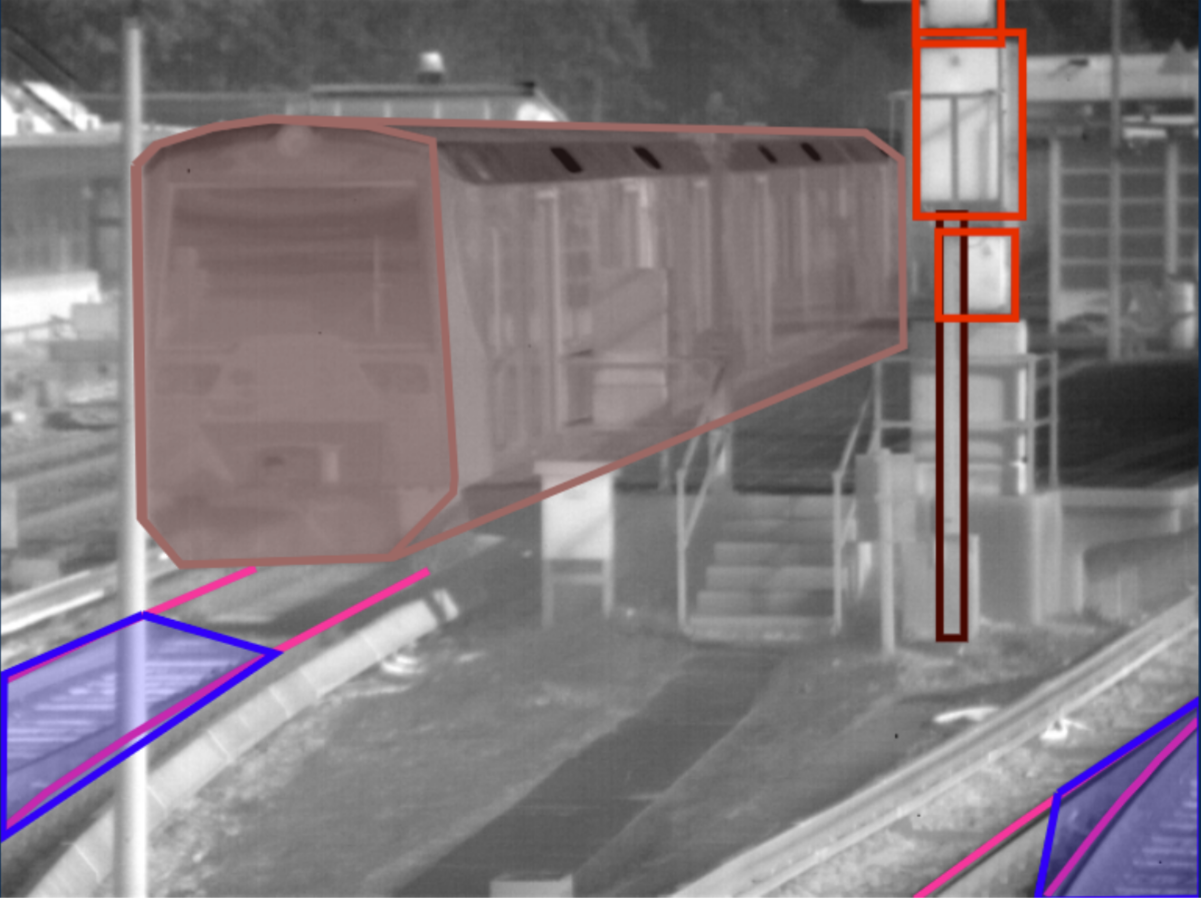
\includegraphics[width=0.9\textwidth,height=5cm]{PICs/datasets/OSDaR23_dataset/labeled_IR.png}
        \caption{Bild 3}
    \end{subfigure}%
    \hspace{0.05\textwidth}
    \begin{subfigure}{0.45\textwidth}
        \centering
        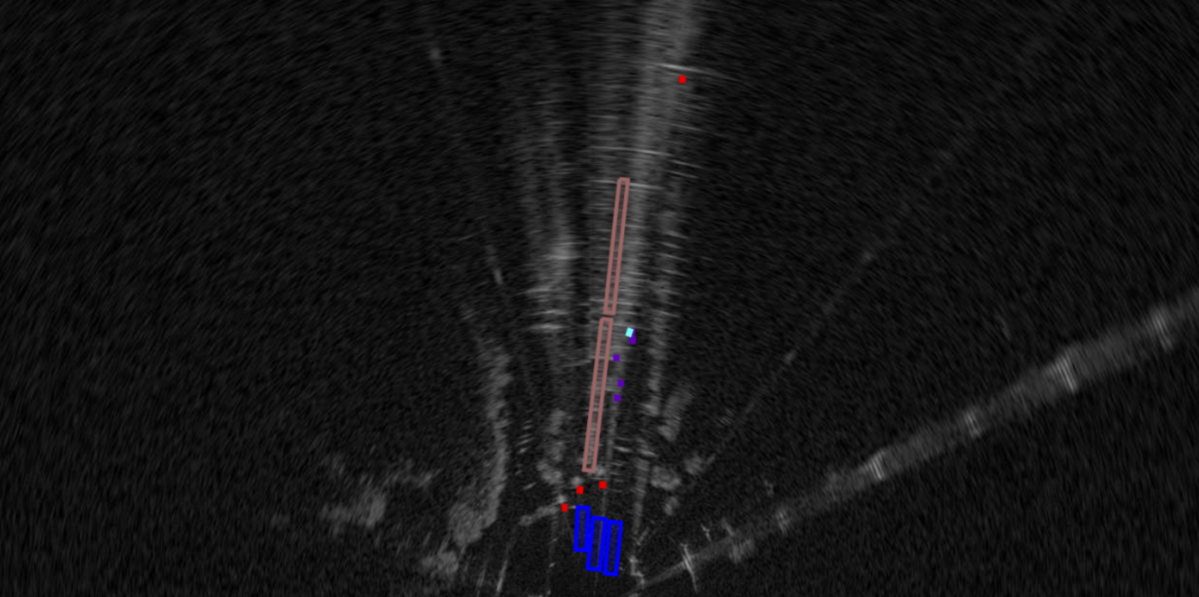
\includegraphics[width=0.9\textwidth,height=5cm]{PICs/datasets/OSDaR23_dataset/labeled_Radar.png}
        \caption{Bild 4}
    \end{subfigure}
    
    \caption{OSDaR23 labels skaliert}
\end{figure}

% TEP-Net annotations
\subsubsection{TEP-Net dataset}
\label{subsubsec:TEP-Net_dataset}

\cite{tepNet2024} presents the \ac{TEP}-Net dataset.
The problem this paper aims to solve is rail track prediction.
This differs from all previously mentioned datasets.
No dataset but \cite{tepNet2024} provides information, which distinguishes possible rails in the image from the one the train actually follows.
Since RailSem19 is the most popular dataset in the rail domain, it is used as initial point.
A total of 7917 images were taken from RailSem19.
The remaining 583 were excluded because they are taken from unusual perspectives or it is unclear which track the train is on or would continue on.
Examples of such images are shown in \ref{tep-net_aussortiert}.
These images are excluded simply by not annotating them.
For annotation a new labeling format is created.
Two classes \textit{rail\_right} and \textit{rail\_left} give information about where the tracks of the train  run.
All other rails which might be in the image are ignored.
These two classes consist of poly lines, which are annotated by the corresponding x and y pixel coordinates of the image.
Only the tracks on which the train is located are labeled.
Even if a switch appears in the image and the train would travel over it, only the tracks in the correct direction are further labeled.
This way, switches are indirectly included in this dataset, providing information on the direction a train would continue, even though there is no explicit label for switches.
The poly lines start from lowest pixel row of the images and extend up to a specific horizon line.
Above this horizon further labeling is not possible.
This may occur for various reasons.
The first reason can be an obstruction of the view by the environment or other trains, as shown in \ref{fig:tep-net-annotated-images}.
Since the images are sourced from YouTube videos, it is also possible that the resolution becomes too low in the distance for separately identifying both rails.
Another reason is when it is not possible to determine the direction in which the track continues based on a switch present in an image.
This can happen due to low resolution or unfortunate camera angles.
These cases may be labeled as \textit{switch-unknown} in the original RailSem19 dataset for example.
Here, the polylines stop before the switch.
The polylines from this annotation can then be converted into several different labels using preprocessing algorithms.
On one hand, they can be directly used as polylines.
On the other hand, they can be transformed into a mask for segmentation tasks by filling in the area between the lines.
A third application would be to convert this mask into a grid for classification tasks.

\begin{figure}[H]
    \centering
    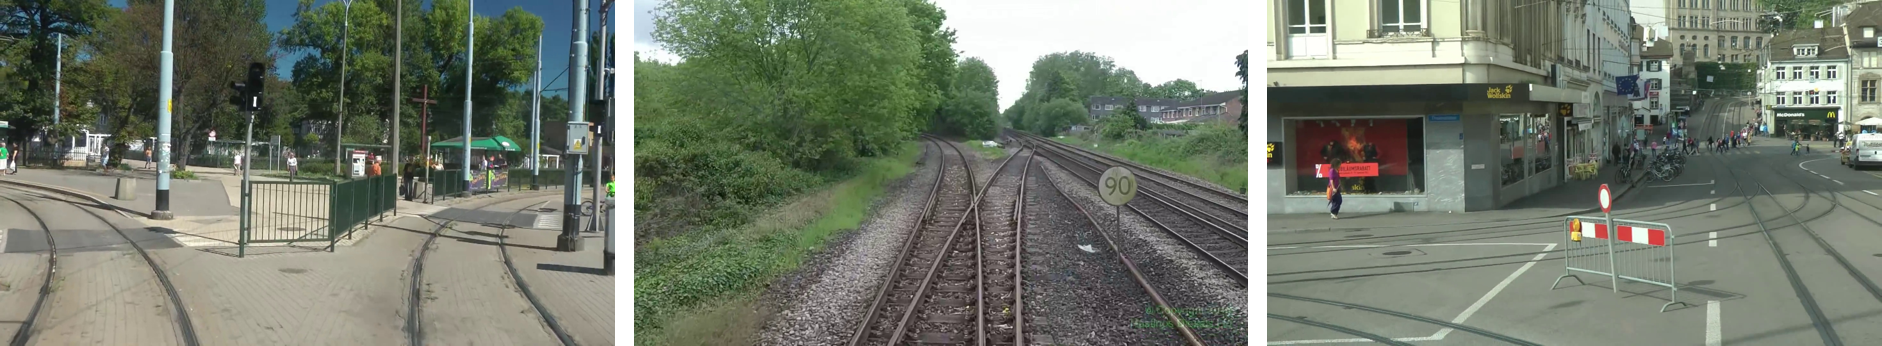
\includegraphics[width=\linewidth]{PICs/datasets/TEP_dataset/TEP-Net dataset bilder aussortiert.png}
    \caption{Examples images from RailSem19, which are not included in the \ac{TEP}-Net dataset due to unclear circumstances about the trains direction. \cite{tepNet2024}}
    \label{tep-net_aussortiert}
\end{figure}


\begin{figure}[H]
    \centering
    
    % Erste Reihe
    \begin{subfigure}{0.328\textwidth}
        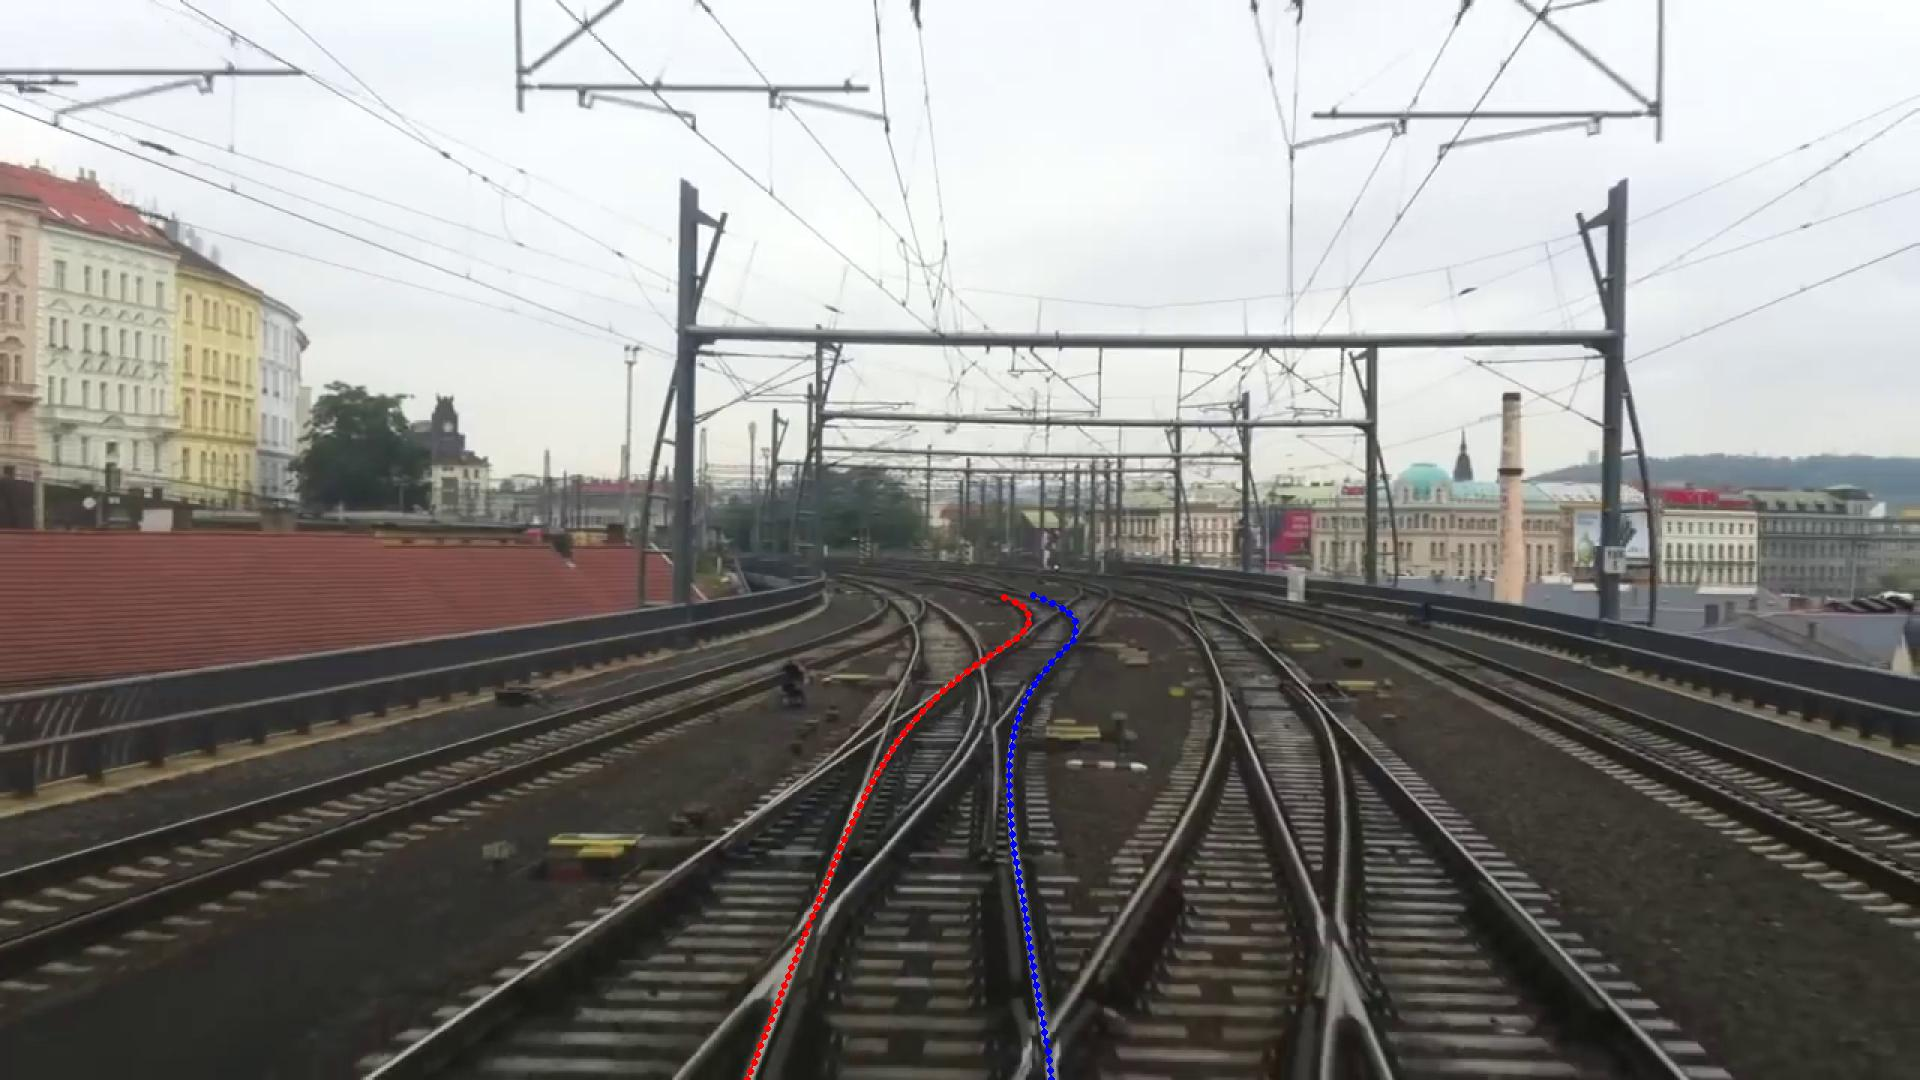
\includegraphics[width=\linewidth]{PICs/datasets/TEP_dataset/annotated_rs00007.jpg}
    \end{subfigure}
    \hfill
    \begin{subfigure}{0.328\textwidth}
        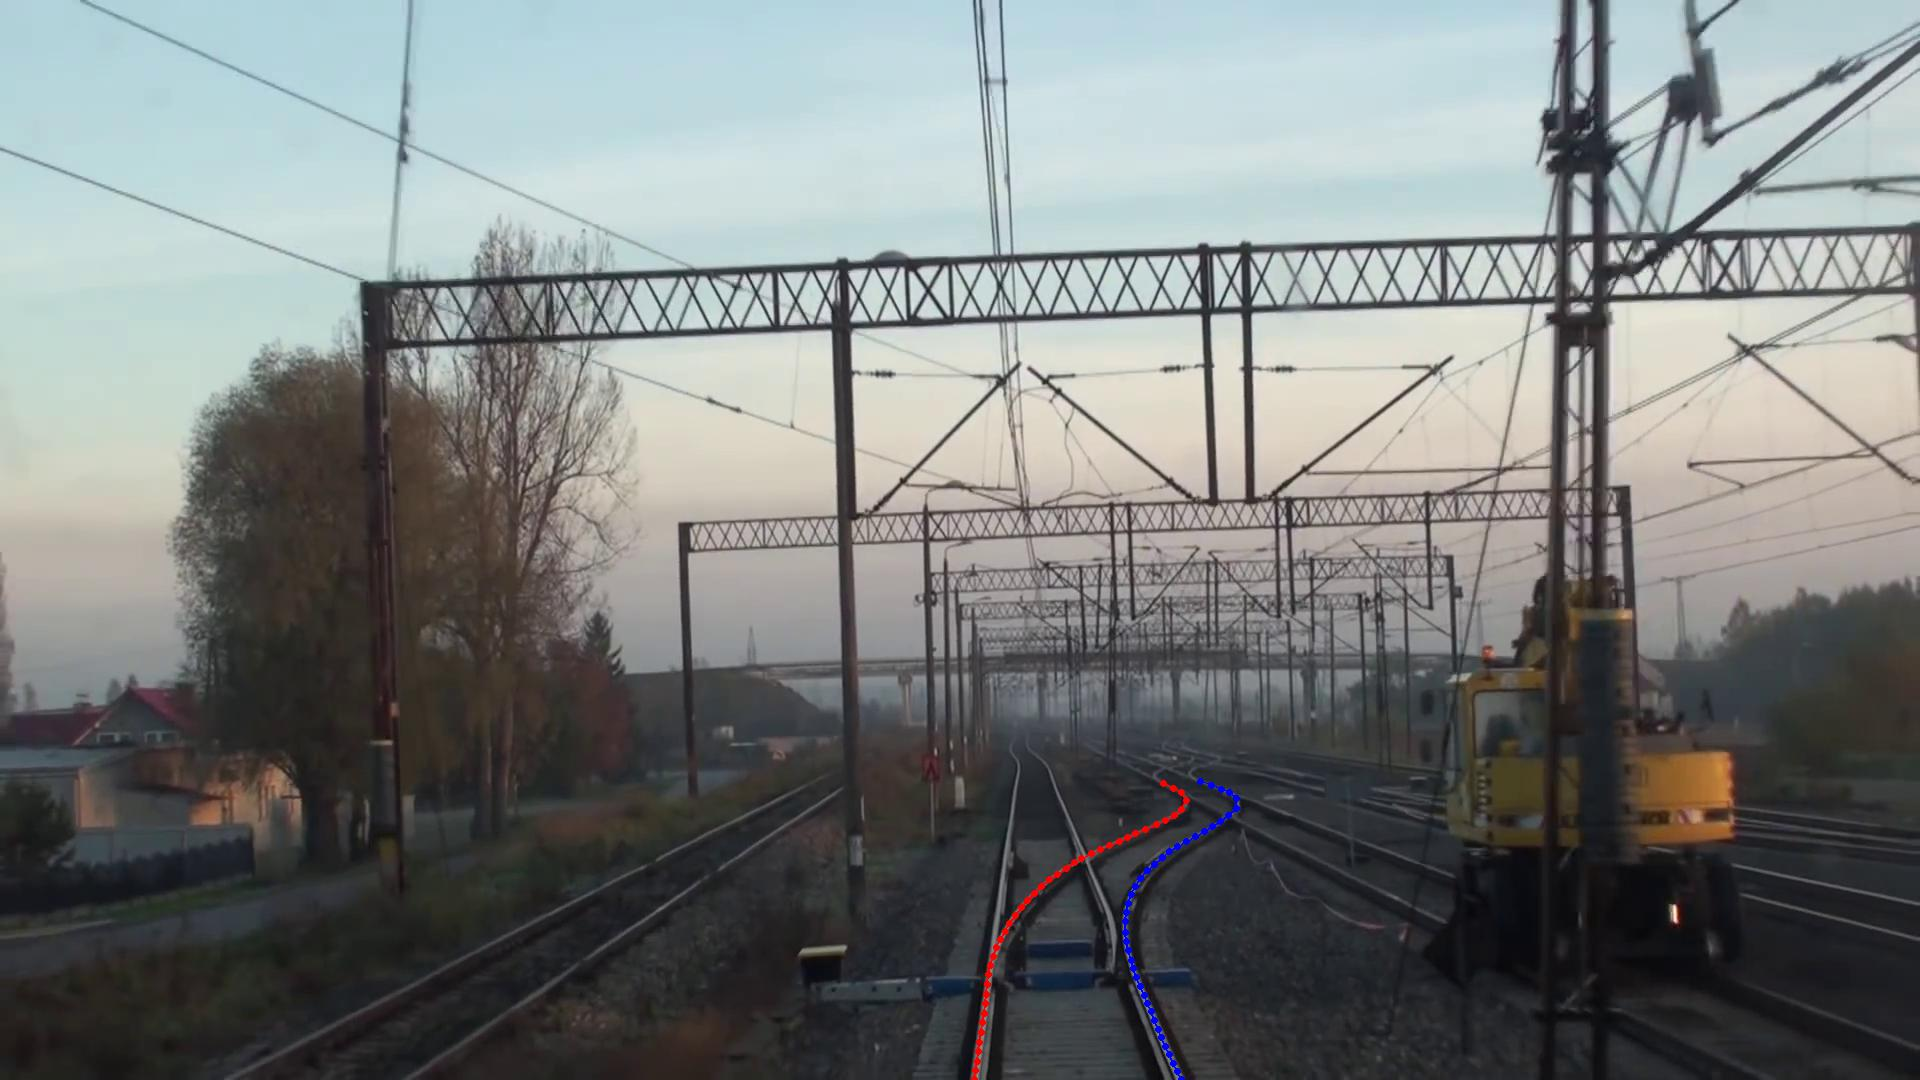
\includegraphics[width=\linewidth]{PICs/datasets/TEP_dataset/annotated_rs00107.jpg}
    \end{subfigure}
    \hfill
    \begin{subfigure}{0.328\textwidth}
        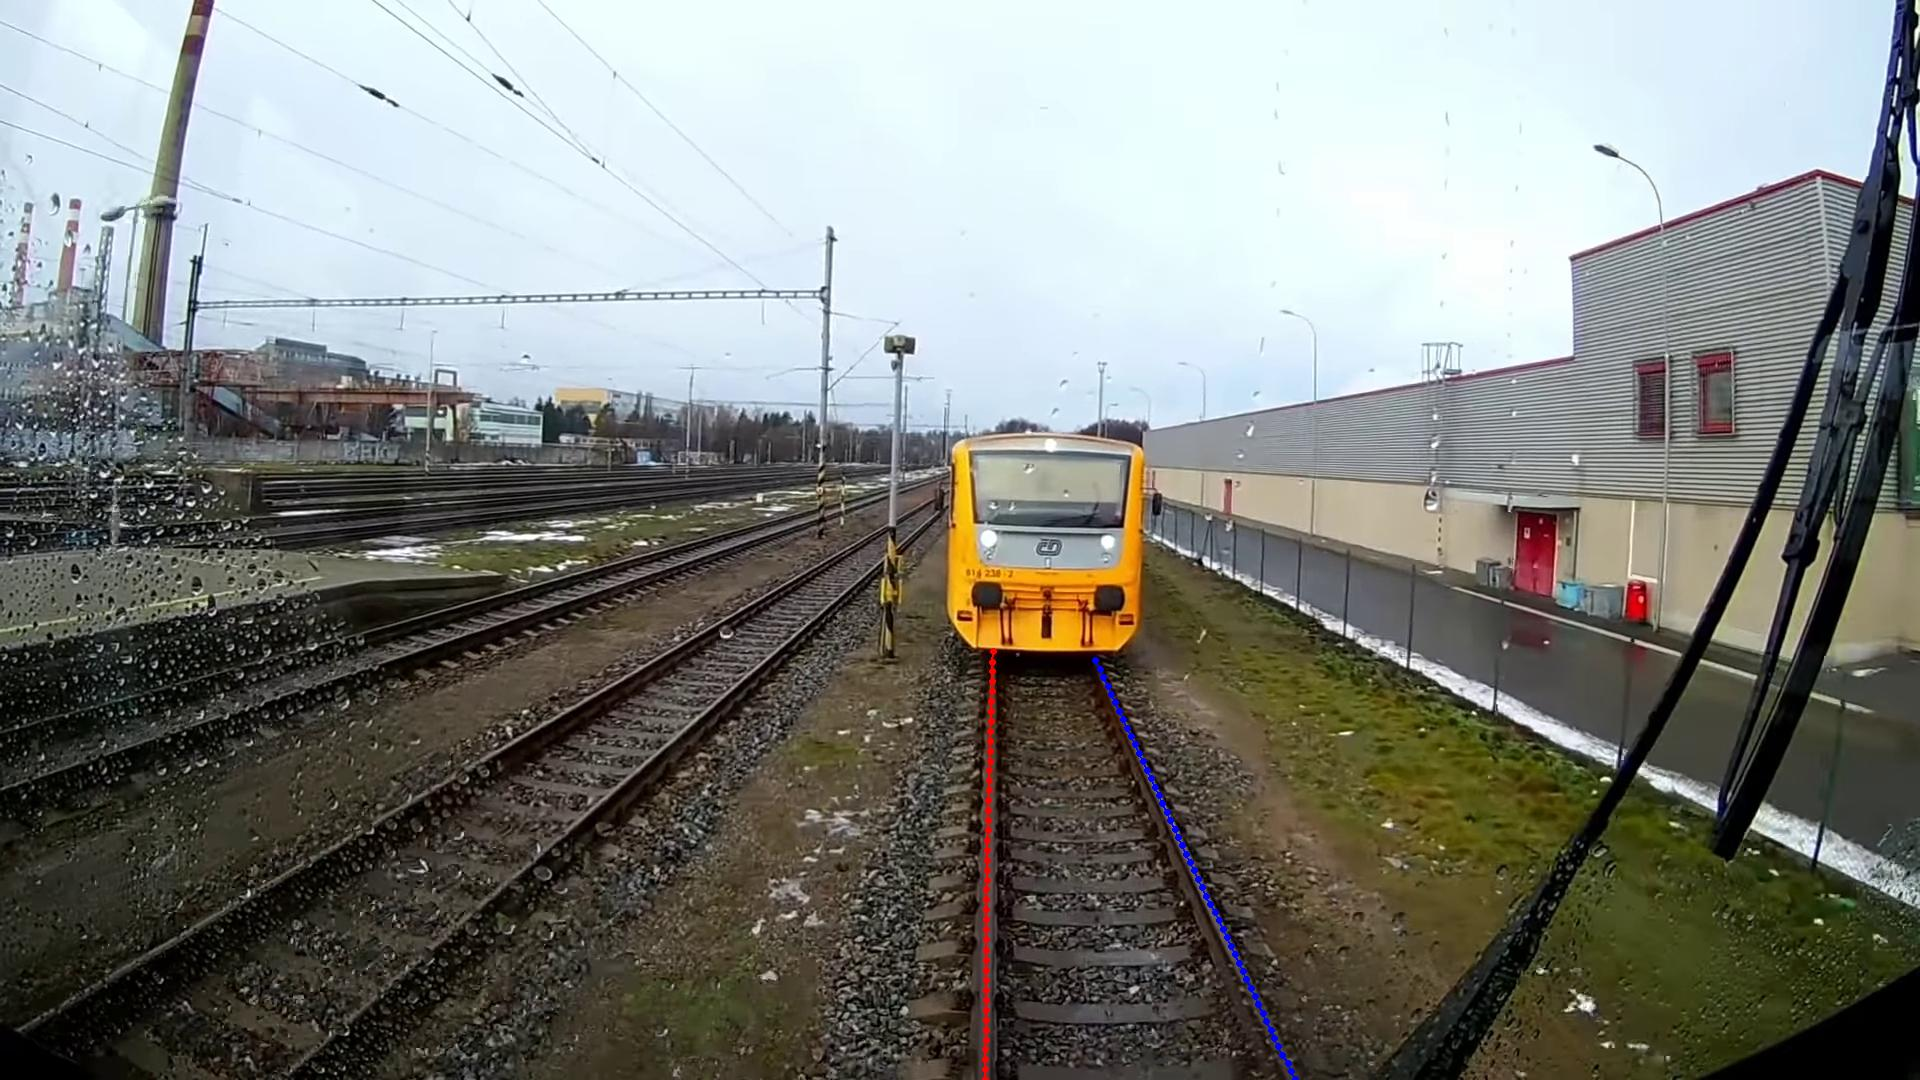
\includegraphics[width=\linewidth]{PICs/datasets/TEP_dataset/annotated_rs00244.jpg}
    \end{subfigure}

    \vspace{0.1cm} % Größerer Abstand zwischen den Reihen

    % Zweite Reihe
    \begin{subfigure}{0.328\textwidth}
        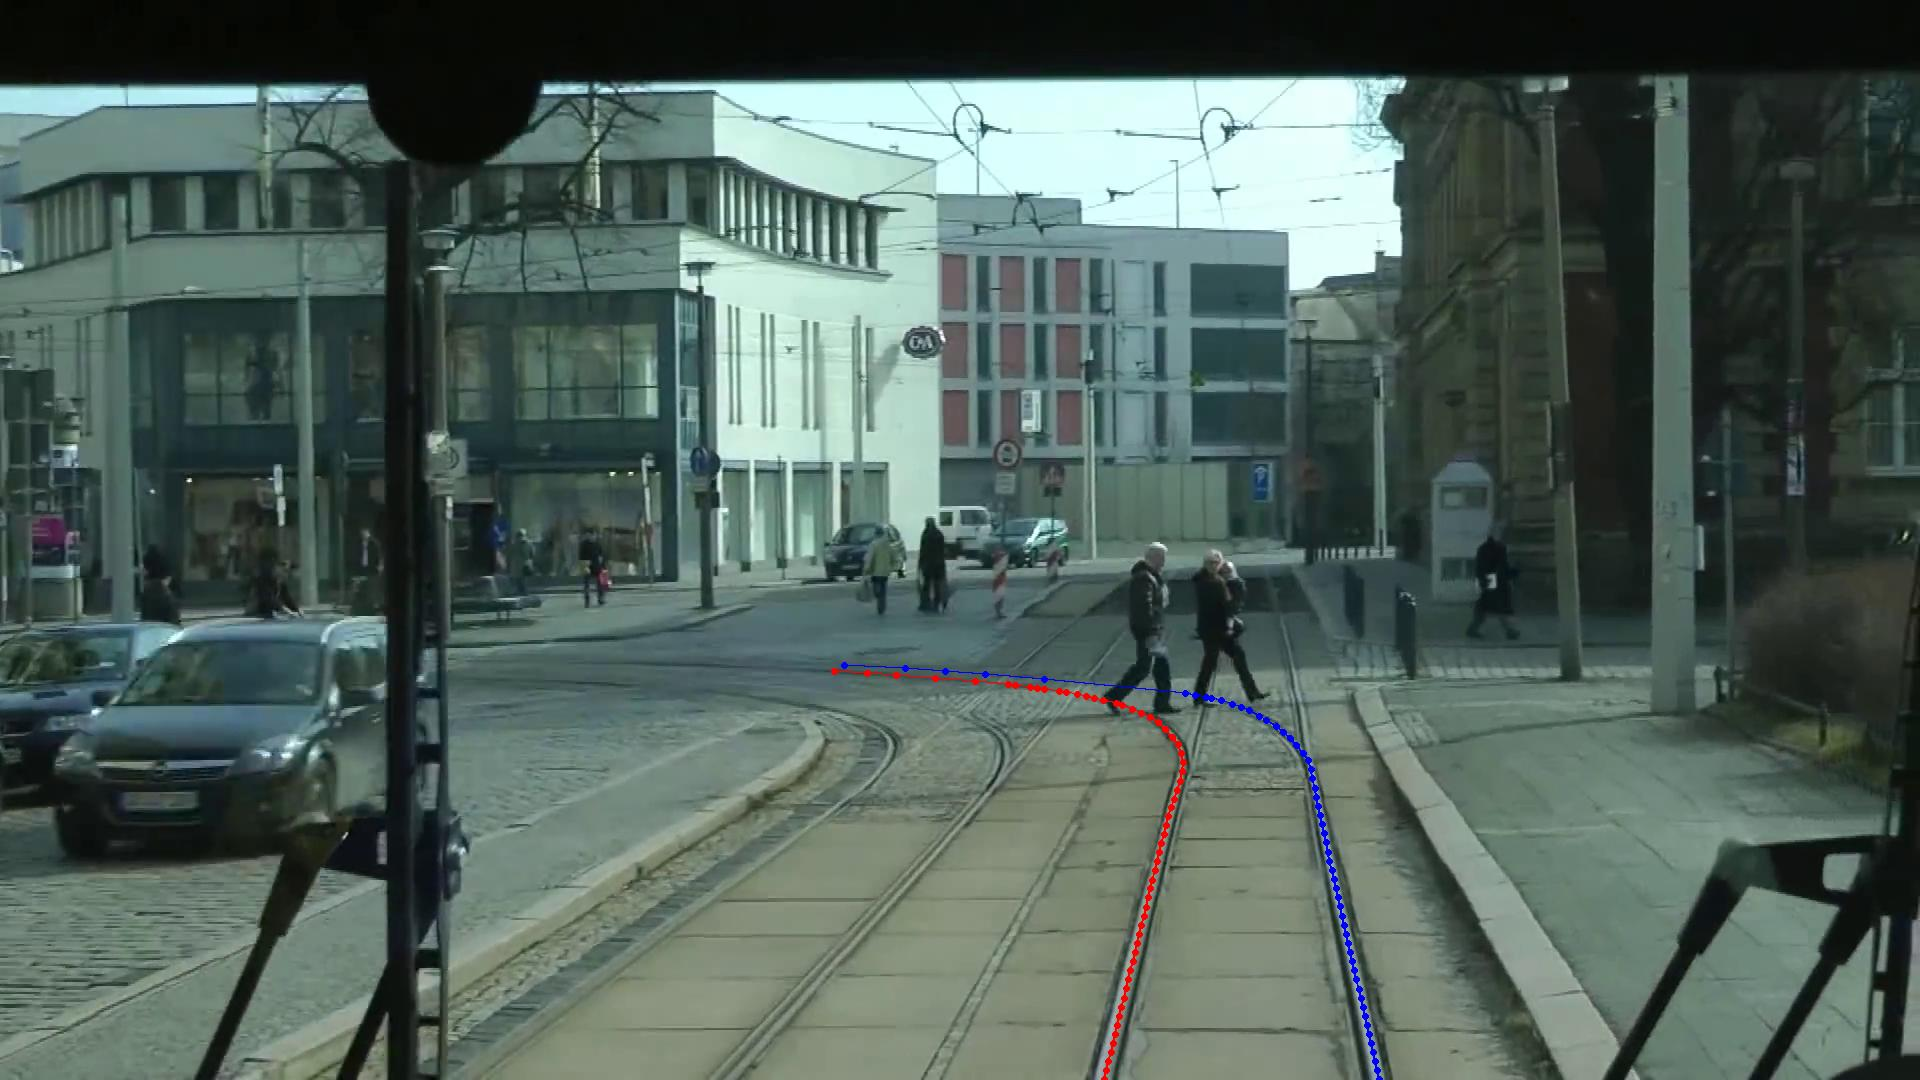
\includegraphics[width=\linewidth]{PICs/datasets/TEP_dataset/annotated_rs00284.jpg}
    \end{subfigure}
    \hfill
    \begin{subfigure}{0.328\textwidth}
        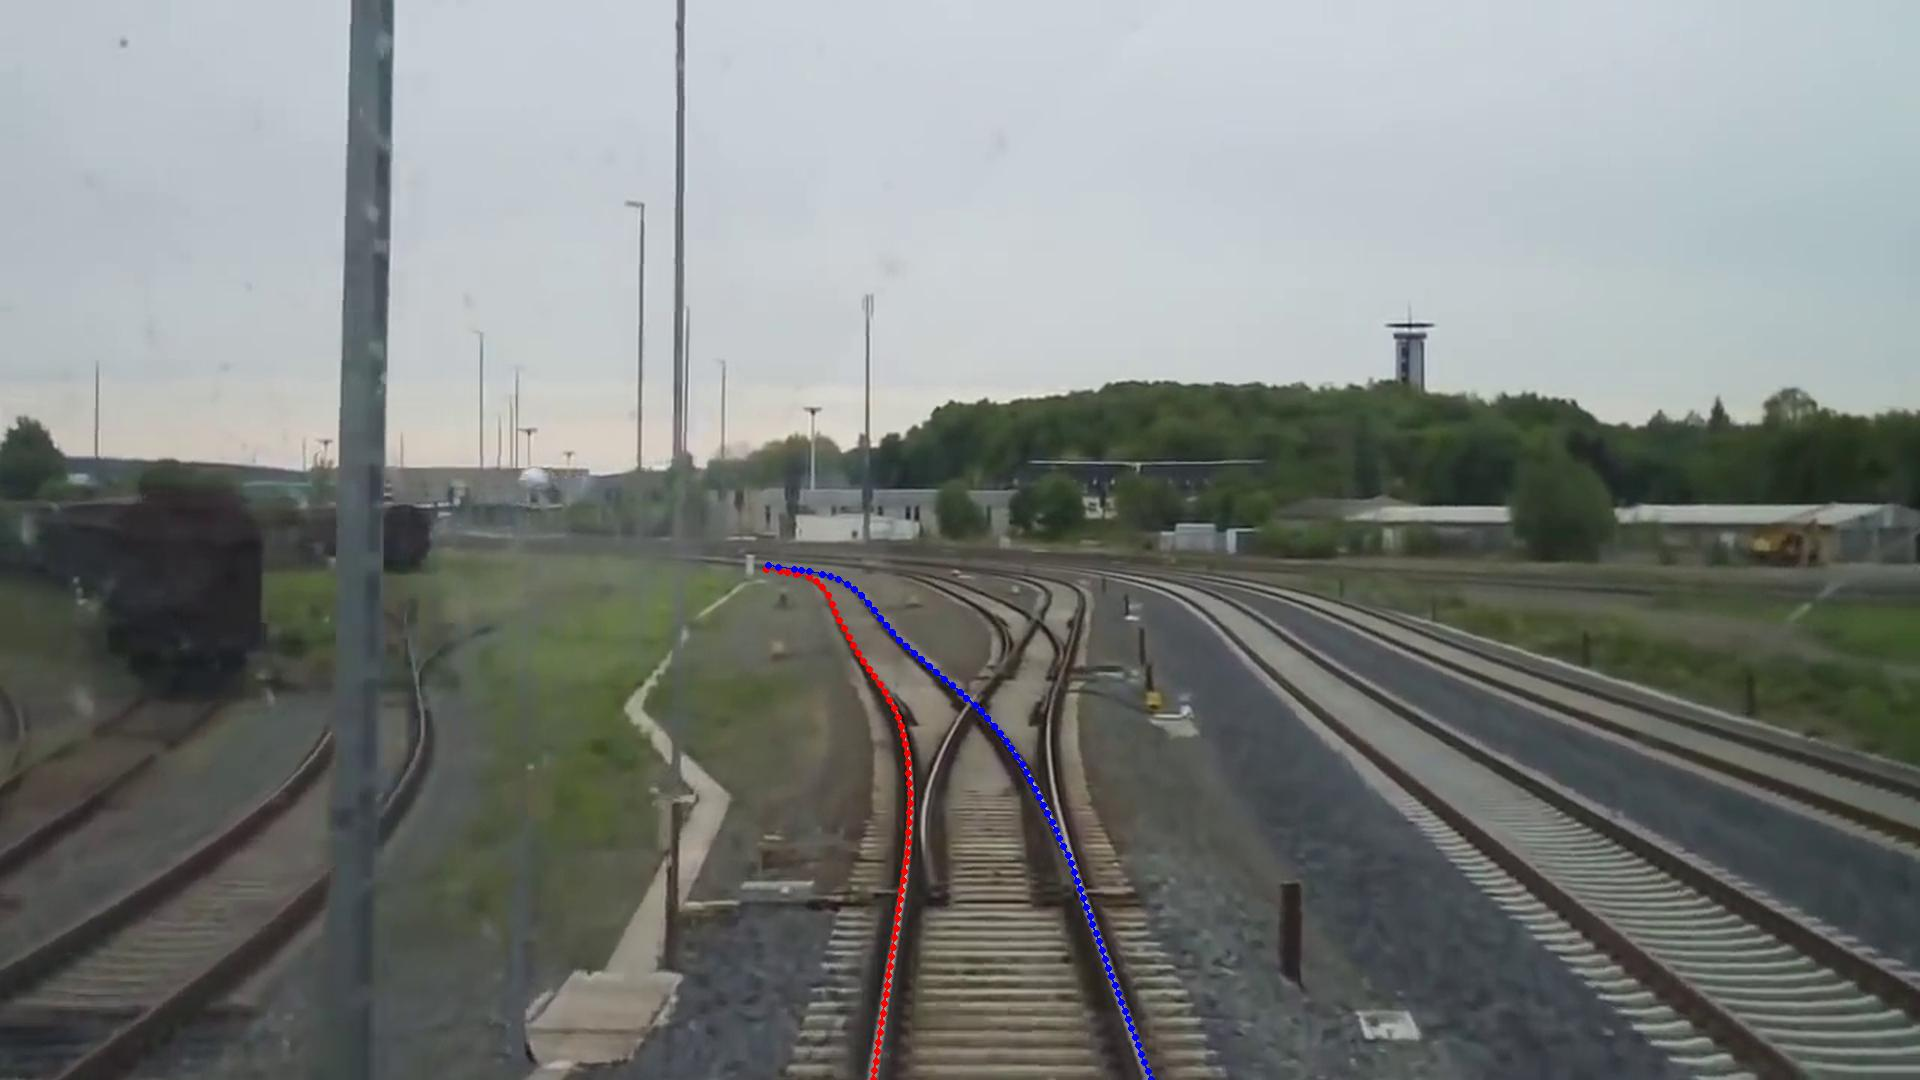
\includegraphics[width=\linewidth]{PICs/datasets/TEP_dataset/annotated_rs00256.jpg}
    \end{subfigure}
    \hfill
    \begin{subfigure}{0.328\textwidth}
        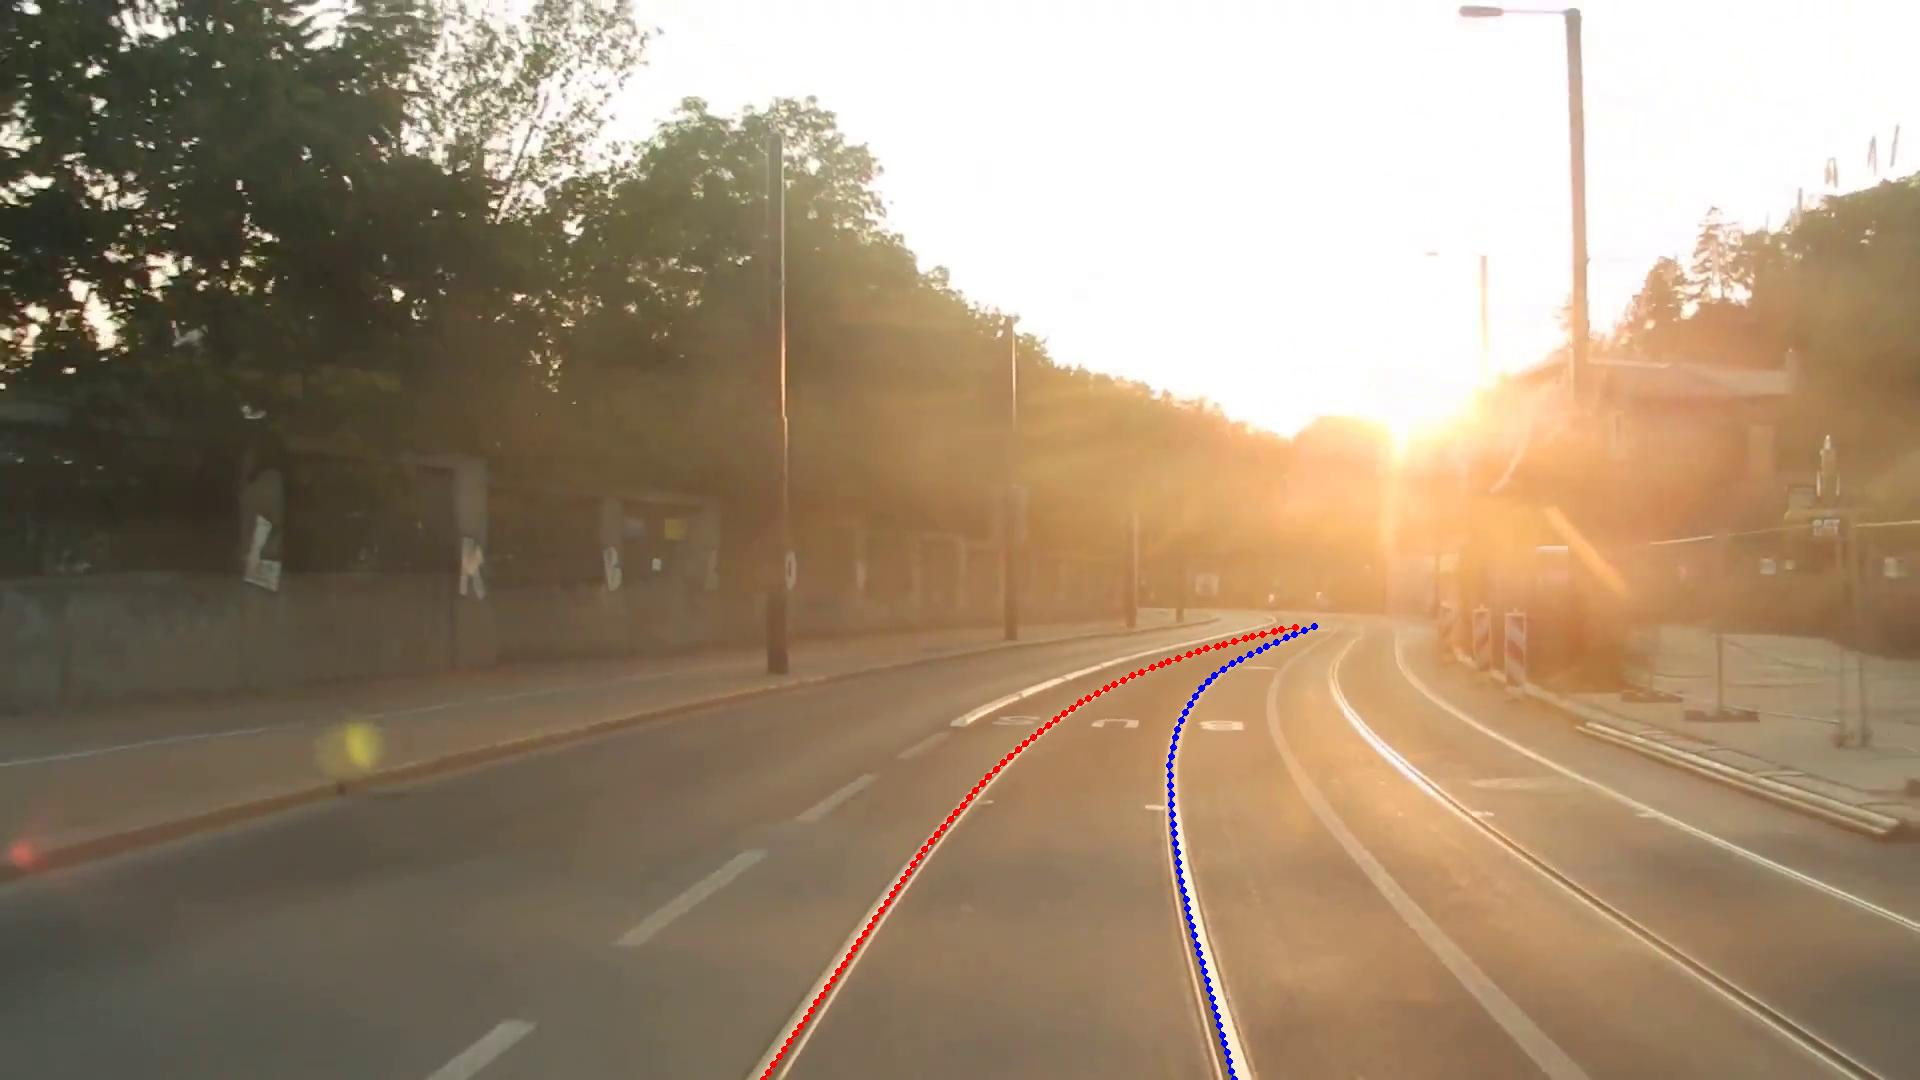
\includegraphics[width=\linewidth]{PICs/datasets/TEP_dataset/annotated_rs00198.jpg}
    \end{subfigure}

    \caption{\ac{TEP}-Net dataset example images with annotation \cite{tepNet2024}}
    \label{fig:tep-net-annotated-images}
\end{figure}

\textbf{notes wo alles ist}

\begin{itemize}
    \item Railroad Segmentation Dataset (RSDS) --> in RailNet: A Segmentation Network for Railroad Detection fertig
    \item RailSem19 in RailSem19 fertig
    \item RailVID in RailVID fertig
    \item RailSet in RailSet \& Application of Rail Segmentation in the Monitoring of Autonomous Train’s Frontal Environment fertig
    \item Rail-DB (compared to RSDS) --> Rail Detection: An Efficient Row-based Network and A New Benchmark fertig
    \item OSDaR23 in OSDaR23: Open Sensor Data for Rail 2023 fertig
    \item TEP-net dataset fertig
    \item
    \item RailSet -> Segmentation \& Anomaly detection
    \item Application of Rail Segmentation in the Monitoring of Autonomous Train’s Frontal Environment -> RailSegmentation (only rails and trackbed)
\end{itemize}

%%%%%%%%%%%%%%%%%%%%%%%%%%%%%%%%%%%%%%%%%%%%%%%%%%%%%%%%%%%%%%%%%%


%%%%%%%%%%%%%%%%%%%%% Baseline Paper %%%%%%%%%%%%%%%%%%%%%

\clearpage                                                       % Beginne neue Seite
\section{Baseline Paper}
\label{sec:baselinepaper}

To do justice to the contributions of \cite{tepNet2024}, it is addressed in a separate section highlighting the paper's specific insights and relevance. 
To the best of the author's knowledge, \cite{tepNet2024} is the only paper in the literature that only filters out the two rails of the train, presenting a solution to the rail track prediction problem.
This is contrary to most literature, in which all rails are often detected without any distinction between different rails.
Efforts in rail detecting with the train's path in consideration have been made in \cite{RailraodSemanticPossibleTracks2020} and \cite{TPENet2023}.
However, because of the assumption that switch states cannot be accurately determined, all "possible rail tracks" are considered in those two papers, leading to complex post-processing.
In \cite{tepNet2024}, the train's rails are defined as the "ego path" and others are ignored.
To realize a system with this output \cite{tepNet2024} presents a novel regression-based approach inspired by autonomous driving applications for road cars.
Contributions include a novel model architecture, new annotations tailored for this use case, a cropping mechanism for inference, a data augmentation strategy, and a custom loss function.

\vspace{0.7cm} % Größerer Abstand zwischen den Reihen

\noindent \textbf{The model architecture} introduced by \cite{tepNet2024} includes a backbone for feature extraction followed by a prediction head.
The head is constructed out of fully connected layers and forms the output at the end.
The output vector includes the $x$-values for the left and the right rail on anchor lines and a value for the horizon line.
\autoref{fig:TEP-Net_sota_models} shows the proposed regression model in the middle.
A more detailed description is given in \autoref{subsec:baselineModel}.

\vspace{0.7cm} % Größerer Abstand zwischen den Reihen

\noindent \textbf{New annotations} are labeled for this project, which only considers the "ego-path".
Images are taken from the RailSem19 dataset \cite{tepNet2024}.
For further details of the dataset, please refer to \autoref{subsubsec:TEP-Net_dataset}.

\vspace{0.7cm} % Größerer Abstand zwischen den Reihen

\noindent \textbf{The autocrop mechanism} is developed for inference \cite{tepNet2024}.
This technique delivers the most relevant crop of the input frame according to a running average of previous predictions.
This method is described in more detail in \autoref{sec:autocrop}.

\vspace{0.7cm} % Größerer Abstand zwischen den Reihen

\noindent \textbf{Data augmentation strategies} are deployed for training \cite{tepNet2024}, including methods like image color variations and horizontal flips.
Since inference focuses on crops instead of whole images, the training must reflect something similar.
Therefore, a random cropping is also used, dependent on the \ac{GT}.
It allows the model to adapt to different image crops in inference.
All data augmentation methods are described in more detail in \autoref{sec:dataaugmentation}.

\vspace{0.7cm} % Größerer Abstand zwischen den Reihen

\noindent \textbf{The loss function} is tailored to the regression approach and is constructed of two functions.
The trajectory loss, which is responsible for the horizontal error, and the y-limit loss, which considers the horizon line.
Both losses are weighted and added.
Please refer to \autoref{sec:lossFunction} for a detailed description.

\subsection{Comparison other state-of-the-art approaches}

\cite{tepNet2024} compared its approach to promising and common methods in the literature: a segmentation and a classification approach.
To compare the novel regression-based architecture fairly, \cite{tepNet2024} uses the same backbone and replaces the prediction heads, as illustrated in \autoref{fig:TEP-Net_sota_models}.
The segmentation model utilizes a U-Net-like \cite{uNet2015} decoder, which outputs a binary mask with dimensions $1 \times 512 \times 512$.
A binary Dice loss is used for training.
The classification model is inspired by \cite{li2022rail} and follows their settings.
It outputs a $2 \times 64 \times (128 + 1) = 16512$-dimensional vector.
$2$ grids for 2 rails, with a height of $64$ and a width of $128+1$.
The $+1$ is for the background class.
A cross-entropy loss is used to train this model \cite{tepNet2024}.
For experiments, the same dataset is utilized with various preprocessing steps to fit the specific task of the model.

\begin{figure}[H]
    \centering
    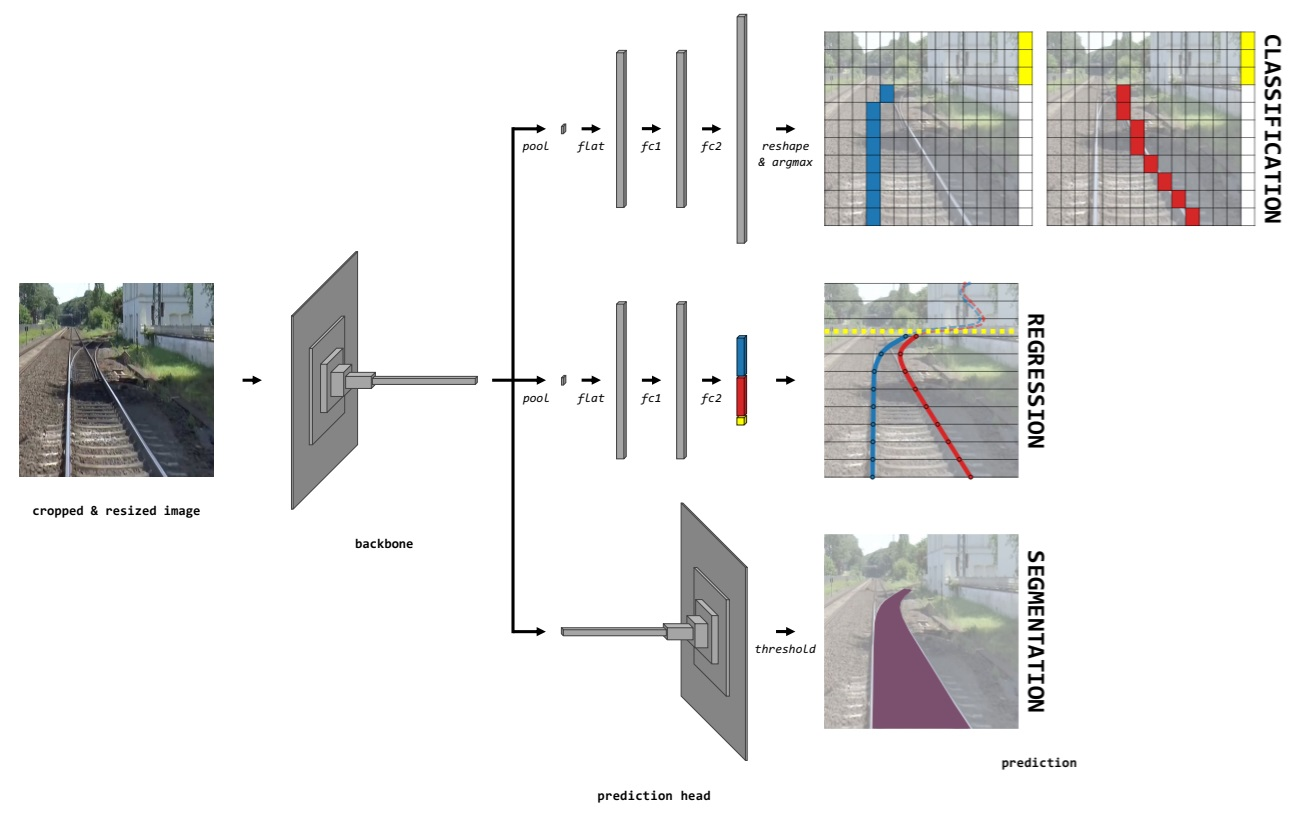
\includegraphics[width=\linewidth]{PICs/Baselinepaper/tep-net_sota_models.jpg}
    \caption{The model architecture is designed to enable a fair comparison between the novel regression model proposed in \cite{tepNet2024} and other \ac{SOTA} approaches.
    All models use the same dataset with preprocessing steps to fit annotation to the model task.}
    \label{fig:TEP-Net_sota_models}
\end{figure}

\noindent Experiments include trainings with different versions of ResNet and EfficientNet backbones.
According to the \ac{IoU}, the segmentation model is the most accurate \cite{tepNet2024}.
However, the performance difference is within a range of only 1.4 percent.
Classification with ResNet18 performs worst.
While segmentation with EfficientNet-B3 achieves the highest accuracy, it is also the slowest.
In terms of speed, the regression-based approach outperforms other models.
Additionally, it proves to be lightweight because of a lower number of parameters and \ac{MACs}.
These characteristics are of great importance for this work's rail track prediction application.
For more detailed results, please refer to \cite{tepNet2024}.

\begin{figure}[H]
    \centering
    \includegraphics[width=0.7\linewidth]{PICs/Baselinepaper/comparison_sota_tep-net.jpg}
    \caption{Comparison between classification (CLS), regression (REG), and segmentation (SEG) models with challenging scenes.
    The worst backbone (ResNet18) is used for this figure to clearly show the difference in behaviors \cite{tepNet2024}.}
    \label{fig:TEP-Net_sota_comparison}
\end{figure}

\noindent Since all three model architectures achieve similar \ac{IoU} scores, \cite{tepNet2024} compares performances on individual challenging scenes.
\autoref{fig:TEP-Net_sota_comparison} visualizes a drop in accuracy when the model becomes unsure.
However, the regression model is the only one that keeps the form of a rail when the track splits and seems to have no issues with obstructions.
This is because the concept of distance in the error between prediction and \ac{GT} is only provided in the regression-based model but is missing in segmentation and classification models.
The cross-entropy loss for classification and the dice loss for segmentation both penalize misclassifications but do not account for increasing distance from the \ac{GT}.
These models work with probabilities, which tend towards extremes under certainty.
When uncertain, segmentation models move closer to a threshold, and classification models show more spread-out probabilities across classes.
The regression approach inherently involves continuous values, which assume averages among uncertain possibilities.
Resulting in a more robust system \cite{tepNet2024}.

\subsection{Limitation}
\label{sec:limitationBaseline}

The main limitation of \cite{tepNet2024} lies in its single-frame-based model architecture.
This model cannot capture temporal context, which becomes problematic when the train encounters a switch.
An example scenario is illustrated in \autoref{fig:limitationSwitch}.
Typically, the model effectively predicts the train's path when approaching switches, with all necessary information contained within the frame.
However, once the train passes over the switch and the start of the switch is no longer visible, the model cannot determine the continuation of the ego path.
Only after a certain duration does the correct track become identifiable again.

\vspace{1cm}

\begin{figure}[H]
    \centering

    % Oberes Grid mit großen Bildern
    \begin{minipage}{0.328\textwidth}
        \includegraphics[width=\textwidth]{PICs/Baselinepaper/limitation_1.png}
    \end{minipage}
    \hfill
    \begin{minipage}{0.328\textwidth}
        \includegraphics[width=\textwidth]{PICs/Baselinepaper/limitation_3.png}
    \end{minipage}
    \hfill
    \begin{minipage}{0.328\textwidth}
        \includegraphics[width=\textwidth]{PICs/Baselinepaper/limitation_5.png}
    \end{minipage}

    \vspace{-0.15cm} % Kleinerer Abstand
    
    % Dritte Reihe nur für die Pfeile (zwischen oberen und unteren Bildern)
    \begin{minipage}{0.16\textwidth}
        \begin{tikzpicture}
            \node[anchor=south] (img) at (0,0) {};
            \draw[->, thick] (1.1,-0.1) -- (1.1,0.1); % Kürzerer Pfeil nach oben für das 1. Bild der unteren Reihe
        \end{tikzpicture}
    \end{minipage}
    \hfill
    \begin{minipage}{0.16\textwidth}
        % Kein Pfeil für dieses Bild
    \end{minipage}
    \hfill
    \begin{minipage}{0.16\textwidth}
        \begin{tikzpicture}
            \node[anchor=south] (img) at (0,0) {};
            \draw[->, thick] (0.5,-0.1) -- (0.5,0.1); % Kürzerer Pfeil nach oben für das 3. Bild der unteren Reihe
        \end{tikzpicture}
    \end{minipage}
    \hfill
    \begin{minipage}{0.16\textwidth}
        % Kein Pfeil für dieses Bild
    \end{minipage}
    \hfill
    \begin{minipage}{0.16\textwidth}
        \begin{tikzpicture}
            \node[anchor=south] (img) at (0,0) {};
            \draw[->, thick] (0.1,-0.1) -- (0.1,0.1); % Kürzerer Pfeil nach oben für das 5. Bild der unteren Reihe
        \end{tikzpicture}
    \end{minipage}
    \hfill
    \begin{minipage}{0.16\textwidth}
        % Kein Pfeil für dieses Bild
    \end{minipage}
    
    % Unteres Grid mit kleineren Bildern
    \begin{minipage}{0.16\textwidth}
        \includegraphics[width=\textwidth]{PICs/Baselinepaper/limitation_1.png}
    \end{minipage}
    \hfill
    \begin{minipage}{0.16\textwidth}
        \includegraphics[width=\textwidth]{PICs/Baselinepaper/limitation_2.png}
    \end{minipage}
    \hfill
    \begin{minipage}{0.16\textwidth}
        \includegraphics[width=\textwidth]{PICs/Baselinepaper/limitation_3.png}
    \end{minipage}
    \hfill
    \begin{minipage}{0.16\textwidth}
        \includegraphics[width=\textwidth]{PICs/Baselinepaper/limitation_4.png}
    \end{minipage}
    \hfill
    \begin{minipage}{0.16\textwidth}
        \includegraphics[width=\textwidth]{PICs/Baselinepaper/limitation_5.png}
    \end{minipage}
    \hfill
    \begin{minipage}{0.16\textwidth}
        \includegraphics[width=\textwidth]{PICs/Baselinepaper/limitation_6.png}
    \end{minipage}

    % Vierte Reihe für die Zeitachse
    \begin{minipage}{1.0\textwidth}
        \centering
        \begin{tikzpicture}
            % Zeit "Time" über dem Pfeil links positionieren
            \node at (-7.5, 0.3) {time}; % Text "Time"
            \draw[-Stealth, thick] (-8, 0) -- (8, 0); % Pfeil von ganz links nach ganz rechts
        \end{tikzpicture}
    \end{minipage}

    % Beschriftung unter dem Grid
    \vspace{0.5cm}
    \caption{Limitation of \ac{TEP}-Net \cite{tepNet2024}. The introduced approach is a single-frame-based model. Therefore, no temporal context can be captured, which leads to uncertainty in prediction when driving over a switch.
    All images are from \cite{limitaion_youtube_video}. A YouTube video, which is also used by RailSem19. It is ensured that none of the frames are included in the dataset, creating a fair test scenario.}
    \label{fig:limitationSwitch}
\end{figure}

\vspace{0.5cm}

\noindent There are two approaches suggested in \cite{tepNet2024}.
The first one includes integrating a confidence score to tell if the model is in a scenario where it is prone to become unreliable.
The second suggested approach is more complete.
It would encounter the temporal component by implementing a model like a \ac{RNN}, that can capture temporal information.
However, \cite{tepNet2024} states that there is no public temporal dataset available, which fits this task.
To the best of the author's knowledge, this statement is correct.
Therefore, a corresponding dataset must also be created, if this approach is pursued.

%%%%%%%%%%%%%%%%%%%%%%%%%%%%%%%%%%%%%%%%%%%%%%%%%%%%%%%%%%%%%%%%%%